% Baylor University Master's Thesis LaTeX template
% Template created by Jonathan Drake (2013)

% This work is the property of Aleksandr Salo,
% Student of Baylor University, Computer Science Department. 
% Copying or using without notifying me is not allowed. 
% Contact email is alexsalovrn at gmail com

% Thesis class, based on report
\documentclass
[
	%short,	% omit front matter
	%draft, 	% draft heading, don't load graphics, etc.
]
{thesis}

% Optional additional packages
%\usepackage{hyperref}
\usepackage{graphicx}
\usepackage{bbm}
\usepackage{tabularx}
\usepackage{adjustbox}  
\usepackage{amsmath}
\usepackage{chicago}
\usepackage{lipsum} % Because this comes with a demo
\usepackage{booktabs}
\usepackage{float}
\usepackage{caption}
\usepackage{subcaption}
\usepackage{epstopdf}
\usepackage{epsfig}
\usepackage{longtable}
\usepackage[]{algorithm2e}
\usepackage{listings}
\usepackage{cleveref}
\usepackage{hyperref}

\newcommand{\argmax}{\operatornamewithlimits{argmax}}

% Thesis parameters
\title{Data Interpretation and Learning on Heterogeneous Behavioral Data Sets.}
\author{Aleksandr Salo}
\holding{B.S.}
\seeking{M.S.}
\degree{Master of Science}
\date{May 2016}

% Administration
\graduateDean{J. Larry Lyon, Ph.D.}
\department{Department of Computer Science}
\departmentChair{Gregory D. Speegle, Ph.D.}

% Supervisor (adviser / mentor)
\supervisor{Erich J. Baker, Ph.D.}
\supervisorTitle{Academic Adviser}

%  Readers (committee members)
\readerOne{Greg Hamerly, Ph.D}
\readerTwo{Enrique Blair, Ph.D}
%\readerOne{Erich J. Baker, Ph.D.}
%\readerFour{...}
%\readerFive{...}

% Abstract
\abstract{
	The Monkey Alcohol and Tissue Research Resource (MATRR) is a rich data repository containing heterogeneous experimental data derived from well-documented non-human primate alcohol self-administration studies. This macaque model has demonstrated categorical drinking norms reflective of human drinking populations. By thorough analysis of the available data we are able to better understand the causative agents, progression and features of alcoholism.
	
	This project presents investigation results separated into two sections: the first describes the rapid discovery and testing of new hypothesis; the second describes the detailed study of predicting future levels of alcoholism based on early (induction) drinking and behavioral data using machine learning techniques. Each study takes advantage of a different set of tools and traces their effectiveness, validity and limitations when describing data in meaningful visual form. We also explore the assignment and cross-examination of data from different sources, and how they aid in generating hypothesis and observing gender and drinking category differences.
}

% Acknowledgments (optional)
\acknowledgements{I want to express my great appreciation to my mentor Dr. Erich J. Baker for guiding me in this research. I also grateful to Dr. Kathy Grant for providing us with data and valuable biological insights.}

% Dedication (optional)
%\dedication{\it To Stacey}

% List of figures (optional)
\makeListOfFigures

% List of tables (optional)
\makeListOfTables

% Document body
\begin{document}

	% Chapters
	\chapter{Introduction}

\section{Problem Domain and Motivation}
Alcohol use disorder (AUD) is a worldwide public health concern and estimated to be the third largest preventable cause of death in the United Sates \shortcite{mokdad2004actual}. This provides motivation for the extensive study of the causes and characteristics of AUDs since identifying risk factors can help to develop and evaluate AUD prevention and treatment programs. However, quantitative controlled studies on humans are usually not feasible for ethical reasons, and mostly rely on self-reporting in relation to drinking behavior or the associated time frames related to drinking \shortcite{hasin2013dsm}. Inconsistency of self-reporting qualitative data does not allow for robust statistical analysis. 

To better understand and model the individual differences in severity of AUDs, a non-human primate (NHP) macaque model of oral alcohol self-administration was developed \shortcite{grant2008drinking}. This macaque model has demonstrated to be reflective of human drinking populations in its categorical drinking norms \shortcite{baker2014chronic}. The Monkey Alcohol and Tissue Research Resource (MATRR)\footnote{Available online: \url{www.matrr.com}} is a data repository and analytics platform for detailed experimental data derived from such NHP alcohol self-administration studies \shortcite{daunais2014monkey}. Specifically, a wide range of data can be collected and collated across individual animals and animal cohorts within the context of a well-defined schedule-induced polydipsia (SIP) model for establishing drinking to intoxication \shortcite{grant2008drinking}. Such data includes subject's drinking pattern, drinking behavior, age, and physiological response to intoxication during the induction period. Overall, MATRR provides a rich volume of heterogeneous data for statistical analysis. 

Analyzing detailed biological data from MATRR requires thorough and efficient strategies which handle the associated complications. The main difficulties are: 
\begin{itemize}
	\item Large volumes: over 20 GB of normalized data in the database.
	\item Heterogeneity: animals of different species, data from various experiments and multiple sources.
	\item Inconsistency: naturally inconsistent data in addition to many human and machine errors produced during the experiments stage or later during the data consolidation stage.
	\item Uncertainty: we do not know in advance whether the data is useful or not. Using meaningless data may hurt the model; not using meaningful data may lead to lower accuracy.  
\end{itemize} 

In this research we try to address this issue by using and evaluating available data analytics tools, combining them and developing novel models. 

\section{Research Objectives}
Our ultimate goal is to prevent negative effects associated with AUDs via learning more about alcoholism, its causes, accompanying characteristics and consequences in primates. To achieve this goal we need to be able to cope with difficulties of analyzing large volumes of heterogeneous data from repositories such as MATRR. Thus, the objectives for the present research are:
\begin{itemize}
\item To describe data in convenient, meaningful and representative visual form.
\item To align (correlate) data from different sources to cross examine the effects of various factors on primate drinking.
\item To use data analysis tools for generating hypothesis.
\item To understand whether or not early data associated with alcohol introduction is predictive of the future levels of alcoholism. 
\item To see whether there is a difference in drinking patterns in males versus females, and low drinking animals versus high drinking animals.
\end{itemize} 


\section{Thesis Structure}
The current chapter overviews the problem domain and motivation. The second chapter highlights the previous work on which present research relies and provides comparison between this and earlier studies. The literature overview includes diverse set of papers in both biological and computer science domains. The third chapter presents the building blocks of the present research: materials, tools and methods used to conduct the investigation, and a  novel two-step model for classification on sparse datasets with small sample sizes. Chapter four introduces the qualitative and quantitative results of several studies along with supporting tables and figures. Lastly, chapter five provides a discussion about the effectiveness and validity of the tools,  their limitations, results evaluation and ideas for future work. 

	\chapter{Literature Overview}
Present research relies on, uses and tests the validity of the results in the prior studies regarding the ethanol self-administration animal model. Additionally, we surveyed existing studies that deploy machine learning techniques on biological datasets. This helped to elucidate the benefits and pitfalls in biological applications of machine learning and allowed us to select more appropriate statistical models. 

\section{Drinking Categories}
In this research we ubiquitously use the notion of \textit{drinking category} assigned to each upon the completion of the experiment. Drinking category, a label characterizing the animal to alcohol relationship, is based on quantitative data about the alcohol consumption by the animal during its entire lifetime. Throughout our research we use the animal's assigned drinking category label as \textit{the ground truth for our analysis}. Below is a short overview of how drinking category is computed. 

The current criteria for alcohol use disorders does not include consumption (quantity/frequency) measures of alcohol intake, in part due to the difficulty of these measures in humans \shortcite{baker2014chronic}. Animal models of voluntary oral ethanol self-administration have enabled usage of the highly accurate quantity/frequency measures over prolonged periods of time. In particular, a large multi-cohort population of Rhesus (Macaca mulatta) monkeys (n=31) was analyzed to establish persistent drinking categories based primarily on the following factors:
\begin{itemize}
	\item Daily alcohol intakes normalized in grams per kilogram [g/kg] of the body weight.
	\item Blood Ethanol Concentration\footnote{In each cohort, BEC was measured every fifth day of the experiment.} (BEC) in mg/dl - a measure which is legally used in the United States to determine alcohol intoxication (over 80 mg/dl). 
\end{itemize}

Experimental results show that daily ethanol intake was uniformly distributed over chronic (12 months) access for all animals, yet underlying this distribution of intakes were subpopulations of monkeys that exhibited distinctive clustering of drinking patterns \shortcite{baker2014chronic}. Aiming to define the distinct drinking categories that demonstrate the most stability over time the following classification is used:
\begin{itemize}
	\item Very heavy drinking (VHD) animals are defined by having an average daily ethanol intake exceeding 3 g/kg AND have $\ge 10\%$ of days with an ethanol intake exceeding 4 g/kg.
	\item Heavy drinking (HD) animals are defined by having an ethanol consumption of $\ge 3 g/kg$ for $\ge 20\%$ of days.
	\item Binge drinking (BD), animals are defined by having an ethanol consumption of $\ge 2 g/kg$ for $\ge 55\%$ of days	AND	a recorded BEC $\ge 80 mg/dl$ at least once per year.
	\item Low drinking (LD) animals are defined as not BD, not HD, and not VHD.
\end{itemize} 

As previously published, this way of classifying animals \textit{shows the most stability over time}. However, it is important to note, that such artificially defined drinking categories is not an objective reality, which is important when analyzing the results described in \cref{section:predicting-drinkers}.


\section{Scheduled Induction Predicts Chronic Heavy Drinking}
The objective of the following experiment is to characterize a large number of behavioral and organismal variables related to drinking during the initial exposure to alcohol and determine which, if any, variables could predict which monkeys would become chronic and heavy drinkers \shortcite{grant2008drinking}. The study uses Principal Component Analysis (PCA) in order to reduce the dimension of predictors and regression models to correlate quantitative attributes with a future drinking category. Additionally, to better utilize the fact that data describes drinking behavior as a continuous process, functional PCA (FPCA) methodology is used. In FPCA the longitudinal pattern of each predictor is decomposed as a mean curve (counterpart of mean vector as in PCA) plus linear combinations of functional PCs (FPCs, counterpart of principal components or PCs as in PCA).

The above study finds that the first 5 principal components with the highest predictive power are: number of ethanol bouts (defined as less than 300 seconds between consumption of EtOH), largest ethanol bout volume, percentage of the 1.5 g/kg dose taken in the largest bout, water intake during the rest of the day, and the number of pellets delivered in State 1 (under the FT 5 minutes schedule) \shortcite{grant2008drinking}. 
%It is not clear from the paper how this attributes were restored from the principal components which were used to reduce dimensionality in the first place. 

One objective of our study is to predict chronic heavy drinking based on scheduled induction data, but using a broader tool set - machine learning algorithms. Another difference is in the number of subjects used: the former study uses 10 animals from one cohort, while we analyze 50 animals from 7 different cohorts.

\section{Age and Sex As Factors in AUDs}
The effect of early initiation of drinking on the risk of AUDs has been debated in many studies. In a recent study it was shown that there is a robust association between age at first drink and the risk of AUD \shortcite{dawson2008age}. The authors argue that it appears to reflect willful rather than uncontrolled heavy drinking, consistent with misuse governed by poor decision-making and/or reward-processing skills associated with impaired executive cognitive function. Since in our research we have access to the information about the age of first alcohol intoxication we are able to directly test this particular finding. In addition, the above mentioned study is based on the \textit{longitudinal self-reporting data} from the National Epidemiological Survey on Alcohol and Related Conditions. In contrast, our study is based on quantity/frequency data which introduces less bias. 

Another factor that is often debated is the role of sex in alcoholism. In one recent study, which uses a two-factor ANOVA model on the subset of the subjects used in our research, the extent of sex differences was greater than previously reported with nonhuman primates \shortcite{vivian2001induction}. Authors note that although ethanol intakes were lower in females compared with males, this diminished consumption of ethanol is not without its consequences. Preliminary data demonstrated \textit{profound changes in menstrual cycle quality} that were associated with higher ethanol intakes. These perturbations in ovarian progesterone in heavier-drinking female cynomolgus monkeys are consistent with disruptions of reproductive function observed in humans and previously documented in rhesus monkeys \shortcite{vivian2001induction}. Since we are increasing the sample size by using five cohorts we are able to use machine learning tools to test sex as a factor in developing AUDs. 


\section{Machine Learning in Biology}
Machine learning (ML) has gained momentum over recent years in many different spheres of research. ML is broadly defined as a set of techniques that allow computers to \textit{learn} without being explicitly programmed \shortcite{simon2013too}. By learning we understand the ability to make predictions on general data after seeing it partially. ML algorithms aim to build a model based on example inputs and make data-driven predictions. That approach contrasts with other statistical methods where model is a set of strictly static instructions. ML, however, often uses available statistical tools and rather extend than replace them. 

Recent work in computational biology has seen an increasing use of ML, specifically ensemble learning methods, due to their unique advantages in dealing with small sample size, high-dimensionality, and complex data structures \shortcite{yang2010review}. However, in bioinformatics, machine learning is predominantly applied into the main topics of gene expression, mass spectrometry-based proteomics and gene-gene interaction identification from genome-wide association studies. In our research we try to apply machine learning to heterogeneous behavioral data sets in order to get insights about the behavioral characteristics that could facilitate early AUD detection. 


 
	\chapter{Materials and Methods}
\section{Data Description}
	Present research is based on heterogeneous behavioral data describing animals from seven different cohorts. Each cohort, having various number of animals of the same sex, was independently undergoing the ethanol self-administration experiment under standardized protocol described later in the text.
	
	\subsection{Animals}
	Fifty rhesus monkeys (Macaca mullata) from the Oregon National Primate Research Center (ONPRC) were used in this study. Animals were both male and female and derived from seven cohorts, designated as ``4", ``5", ``6a", ``6b", ``7a", ``7b", and ``10". Each cohort had animals of the same sex. Table~\ref{tab:data-breakdown} displays the sex of the monkeys corresponding to each cohort, their average age in years, average weight in kilograms, and age at first intoxication, i.e., age when their BEC (Blood Ethanol Concentration) was greater than 80 mg/dl \shortcite{dawson2008age, li2007alcohol}. In the table, \textbf{N} represents the total number of monkeys per cohort and \textbf{n} represents the overall number of monkeys in our analysis.
	
	\begin{table}[htb]
		\centering
		\caption{Breakdown of cohorts used in this study. Weight is the daily average during induction. Age at intoxication is defined as the first BEC over 80 mg/dl.}
		\label{tab:data-breakdown}
		\begin{tabular}{lllllc}
			\hline
			\abovespace\belowspace
			Cohort & N (n=50) & Sex & Age (yrs) & Weight (kg) & Age at intox. (yrs) \\
			\hline
			4 		   & 10 & M & 10.13 & 9.61 & 8.64   \\
			5            & 8 & M & 7.2 & 9.34 & 6.05  \\
			6a           & 6 & F & 5.36 & 5.36 & 4.23 \\
			6b    		& 5 & F & 7.05 & 6.76 & 5.91  \\
			7a           & 8 & M & 5.84 & 8.44 & 4.76   \\
			7b    		& 5 & M & 7.21 & 11.08 & 6.01   \\
			10    		& 8 & M & 6.76 & 5.26 & 5.48   \\ 
			\belowspace \\
			\hline
		\end{tabular}
	\end{table}

	All animals were born into a pedigreed population and remained with their mothers in a multigenerational troop until weaning at about two years of age. All monkeys were continually in a social setting at Oregon National Primate Research Center (ONPRC) and transitioned to individual cages within a laboratory building at least three months prior to the onset of ethanol self-administration according to established protocols \shortcite{helms2014effects}. The age range encompasses late adolescence to early middle age of captive monkeys and data from a subset of these monkeys addressing age as a risk factor for chronic alcohol self-administration has been published \shortcite{helms2014effects}.
	
	Monkeys were housed individually with four cages arranged on a single rack: two cages located above and two below. Monkeys that weighed over 10kg were allowed access to both horizontal cages, but only one drinking panel was affixed to the side of the cage. Each cohort was housed together in the room using multiple racks. All animals had visual and auditory access to other monkeys in the room. Male monkeys were allowed tactile access to adjacent monkeys through grooming grids inserts in the common wall of the cage and female monkeys were allowed two-hour access/day to a common space by removing the horizontal barriers between the cages.
	
	
	\subsection{EtOH Self-Administration Experiment Description}
	The monkeys were induced to self-administer 4\% EtOH (mixed with water) using a schedule-induced polydipsia (SIP) procedure previously described in detail \shortcite{vivian2001induction, grant2008drinking}. Visual representation of the experiment is shown in Figure~\ref{experiment_design}. The dose of EtOH the monkeys were required to consume each day increased every 30 days beginning from 0.5 g/kg to 1.0 g/kg, and finally to 1.5 g/kg. These three stages of 30 days each formed the \textbf{induction} phase.
	
	After the $30^{th}$ session of 1.5 g/kg EtOH the monkeys had concurrent access to EtOH (4\% mixed with water) and water. In other words, animals were to choose between water and alcohol solution. Access was limited to 22 hours a day ensuring animals would have guaranteed sleep time. This phase, when animals had a free choice of drink, was termed \textbf{Open Access (OA)}. Duration of OA varies for each cohort (from six months to 18 months); food, as at least 3 meals per day, was provided during OA \shortcite{grant2008drinking}.
	
	\begin{figure}[ht]
		\centering
		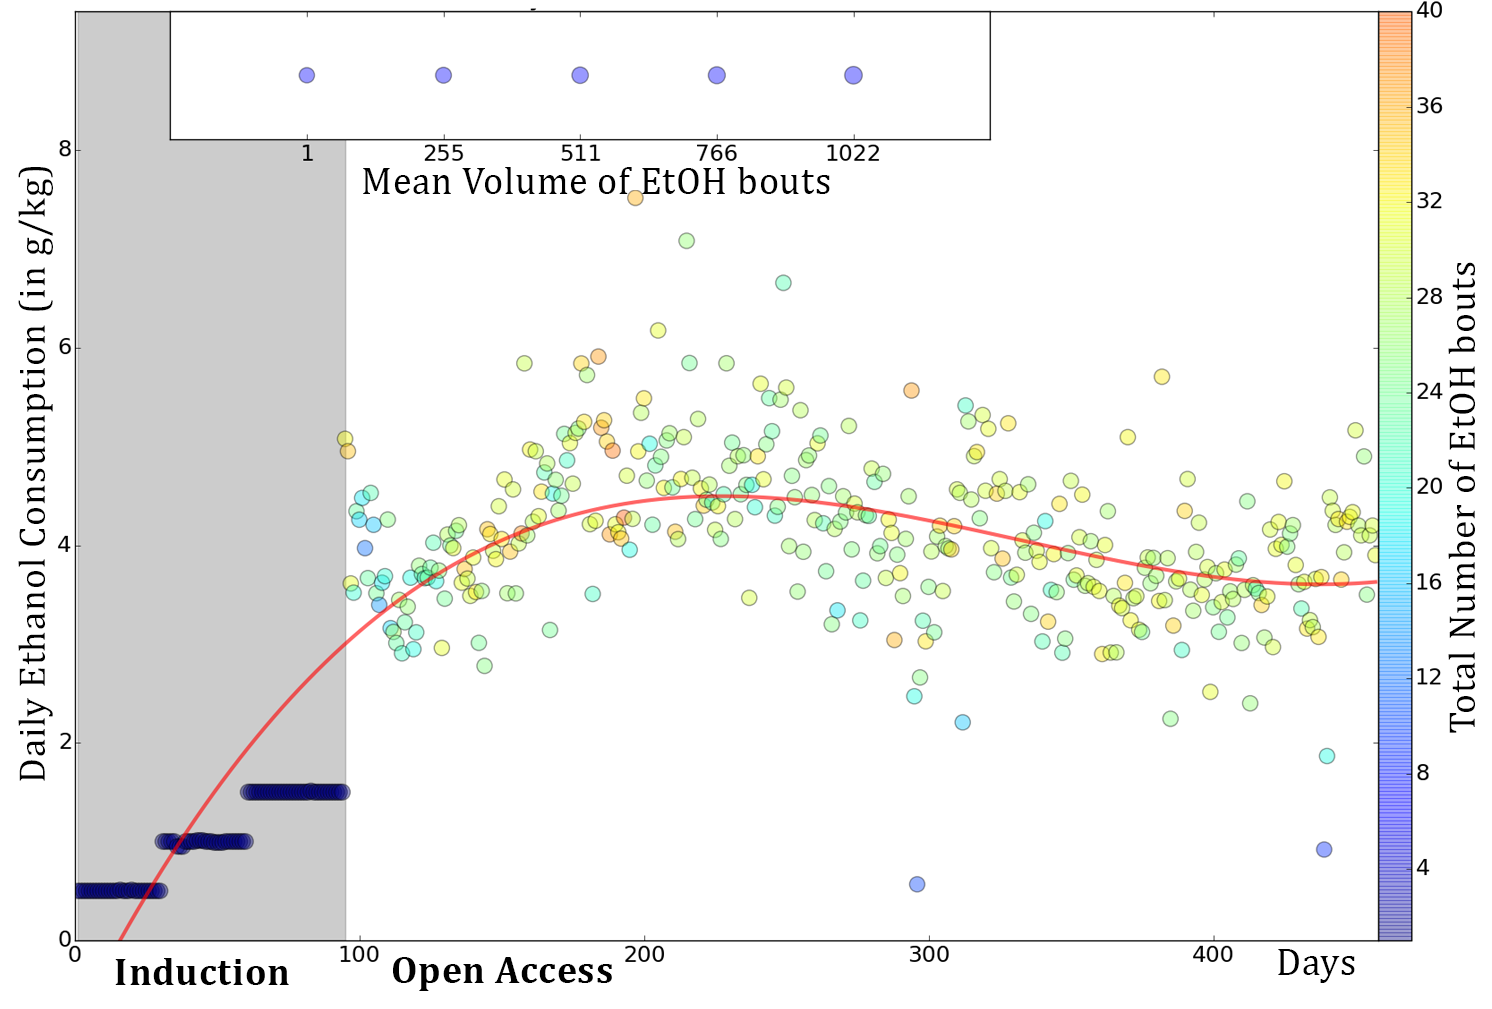
\includegraphics[width=1\linewidth]{figures/experiment_design.png}
		\caption{EtOH self-administration experiment design illustration for one animal. Shaded area represents Induction phase. The rest is Open Access (OA). Points represent aggregated information about one drinking day. A point's position on the Y-axis shows average ethanol consumed that day. The size of the point represents mean volume of ethanol bouts, while color indicates the total number of such bouts during that day.}
		\label{experiment_design}
	\end{figure}
	
	\subsection{Dataset Structure}
	Throughout the experiment magnitude of measurements for food and liquid consumption were taken on daily basis. At the end of the day some attributes were aggregated into mean values, which were more convenient for analysis. Raw data was also stored, which proved to be useful whenever new metric was adopted. 
	
	In earlier research \shortcite{baker2014chronic}, described in chapter 2, \textbf{Drinking Categories (DC)} were assigned to each animal based on quantitative data \textit{during the open access phase}. It was shown that clustering all animals into four DCs (low drinking (LD), binge drinking (LD), heavy drinking (HD) and very heavy drinking (VHD)) captures the most variability of quantity/frequency measures of alcohol intake. The important caveat, however, is that these \textit{DCs are not innate features of the animals, but an arbitrary assigned labels}, which do not necessarily constitute the objective reality. Nevertheless, for the purposes of our research DC serves as an objective function, thus in this paper we treat drinking category labels as the ground truth.
	
		\subsubsection{Drinking Behavior Attributes}
		Present research uses data recorded from approximately 5000 total sessions (over 20 GB of normalized data in the database), one session per day per animal. During every session, detailed information about different relational quantitative attributes was collected for behavioral analysis. Daily averages and other derived attributes were summarized into daily averages as appropriate \shortcite{grant2008drinking}.
		
		Figure~\ref{experiment_design} provides an illustration of the data collected for one animal. Points represent aggregated information about one drinking day: average ethanol consumed, mean volume of ethanol bouts and the total number of such bouts.
		
		Table~\ref{data-selected-attributes} shows a partial list of drinking attributes that explain most of the variation in the data and provided the greatest predictive power, according to the methods described herein. A complete list of all the attributes studied in our research can be found in the Appendix A, Table~\ref{data-all-attributes}. In addition to these quantitative measurements in seconds, milliliters or percentage points, there are several qualitative attributes, which we model with dummy variables.
		
		\begin{table}[!t]
		\centering
		\caption{Partial set of database attributes describing animal drinking behavior during induction. Each variable was summarized daily for 90 days. A complete list is available in the Appendix A, Table~\ref{data-all-attributes}.}
		\label{data-selected-attributes}
		\begin{tabular}{ll}
			\hline
			\abovespace\belowspace
			Drinks (intakes $\le$ 5 sec apart)&	Bouts (intakes $\le$ 5 minutes apart)\\
			\hline
			Number of EtOH drinks& 	Number of EtOH bouts\\
			Average EtOH drink length (sec)&	Average EtOH bouts length (sec)\\
			Average EtOH drink volume (ml)& 	Average EtOH bouts volume (ml)\\
			Median EtOH inter-drink interval (sec)& Median EtOH interbout interval (sec)\\
			Average number of EtOH drinks per bout& Number of H2O bouts\\	 	 
			\belowspace \\
			\hline
			\abovespace\belowspace
			First and Max bout &	Time \& Other \\
			\hline
			Number of EtOH drinks in first bout& Time to reach EtOH allotment (sec) \\
			\% of days EtOH consumed in first bout& Latency to first EtOH drink (sec) \\
			Max bout volume (\% of day's total EtOH) & Number of bouts with max EtOH \\
			Max bout length (sec) &	EtOH in first 10 min. (\% of day total)\\
			Sequence number	of max bout & Average number of H2O drinks in bout \\	 	 
			\belowspace \\
			\hline
		\end{tabular}
		\end{table}

	\subsection{Data Consistency}
	Most of the data was collected using automated processes, which ensured the overall quality and consistency of the data. However, there were two major sources of errors and inconsistency which we had to address: human and machine errors, and natural inconsistency.
	
		\subsubsection{Human and Machine Errors}
		Humans were partially responsible for data aggregation, leading to occasional errors. Lab employees also were to control the environment settings which may produce unplanned variation. Since MATRR absorbs the data from multiple labs and various sources not following data guidelines is an issue. Usage of different operation systems created another set of compatibility problems since data partially were sent into the database in form of spreadsheets. Overall, we tried to spot and fix such errors, if possible, and not to use inconsistent data otherwise.
		
		\subsubsection{Natural Variation versus Inconsistency}
		Since the data describes animal behavior we needed to be careful to distinguish between random natural inconsistencies and variables of interest. For example, animals undergoing a blood drawing are very stressed, which affects alcohol consumption; when animals are sick they change their behavior. These cases may lead to data inconsistency which we want eliminate. On the other hand, females vary their drinking pattern in correlation with the menstruation cycle (this would be further described in the chapter four) which we want to account for.
		
		To ignore the data inconsistency that we can not fix we created exception days which are not used in the studies.
	  
\section{Computational Tools}
	This section presents the parts of the computational apparatus used in this research, their interaction, and their advantages and limitations.
	\subsection{Monkey Alcohol and Tissue Research Resource}
	The Monkey Alcohol and Tissue Research Resource \nobreakdash{(MATRR)}
	is a web system developed primarily in the Python programming language. MATRR was created to store tissues from EtOH and control subjects, empirical data relating to alcohol self-administration, data
	derived from tissue analysis, and data analytics (including data
	mining and data harmonization, and tissue dissemination) \shortcite{daunais2014monkey}. 
	The MATRR serves to close the loop between
	tissue derived from this oral alcohol self-administration model
	and integrated analysis of behavioral, physiological, pharmacological,
	and molecular data by tracking analyses conducted on
	distributed tissues, thus reinforcing tissue selection and experimental
	development by a network of laboratories. Metadata about all animals described in this study, as well as raw and
	semi-processed drinking and behavioral data, are imported in
	MATRR (http://www.MATRR.com) where analysis is performed.
	
	\subsection{Hardware}
	All computations were executed on MATRR’s web and database
	servers. These are twin machines, each running 4 Intel Xeon E5620
	(2.4 Ghz) with 4 cores each, 47 GB RAM, and 1.7 TB disk space in
	a RAID configuration. The hardware design ensures efficiency of the calculations while providing security against the data loss by using non-volatile storage. 
	
	\subsection{Object-Relation Mapping}
	MATRR uses PostgreSQL DBMS, one of the most advanced and efficient open source databases available. All the data manipulation is done via Object-Relation Mapping (ORM) within Django. Django is a high-level Python Web framework that encourages rapid development and clean, pragmatic design. Django includes connectors to the PostgreSQL and allows a developer to treat the relations in the database as if they were objects, and tuples of the relations as if they were object instances. This greatly simplifies and speeds up the data analysis. In conjunction, the advanced DBMS is capable of storing huge datasets as a set of normalized relations securely on non-volatile storage while scientist works with such data as if it was all in the main memory, without any complexity of converting and aggregating data using the Structured Query Language.  
	
	
	\subsection{Data Analysis Tools}	
	\textit{SciPy} is a Python-based ecosystem of open-source software for mathematics, science, and engineering \shortcite{millman2011python}. Present research greatly benefited by using several of its core packages such as Numpy, Pandas and Matplotlib. Numpy was used for efficient statistical computations of mean, variance and correlations.
	
	\textit{Pandas} is an open source, BSD-licensed library providing high-performance, easy-to-use data structures and data analysis tools for the Python programming language \shortcite{mckinney-proc-scipy-2010}. Pandas was created because native Python is great for data preparation, but does not readily accommodate data analysis and modeling. Pandas enables us to carry out entire data analysis workflow in Python without having to switch to a more domain specific language like R. Pandas, however, does not implement significant modeling functionality outside of linear and panel regression, thus present research uses Statsmodels and Scikit-learn libraries.
	
	\textit{Statsmodels} is a Python module that allows users to explore data, estimate statistical models, and perform statistical tests \shortcite{statsmodels2010}. An extensive list of descriptive statistics, statistical tests, plotting functions, and result statistics are available for different types of data and each estimator. Present research took advantage of the Statsmodels' implementation of generalized linear models, validation methods and various statistical tests. 
	
	\textit{Scikit-learn} is an open source Python library containing simple and efficient tools for data mining, machine learning and data analysis \shortcite{scikit-learn}. In particular, present research used the following Scikit-learn implementation of the following models: Support Vector Machines, Random Forests, Gradient Boosting Classifier and Regressor, and others. 
	
	It is worth noting that all the libraries above are easy to use in combination with each other which renders a powerful ecosystem for the fast and efficient data analysis which does not require any costly software licensing. 
	
	\subsection{Visualization Tools}
	\subsubsection{Visualization Libraries}
	All visualizations in this paper were made using Matplotlib and Seaborn python libraries. 
	
	\textit{Matplotlib} is a python 2D plotting library which produces publication quality figures in a variety of hardcopy formats and interactive environments across platforms \shortcite{Hunter:2007}. The Matplotlib community provides a magnitude of examples from scientific research along with the constant improvements and new features. Most of the features of the R (statistical language) visualization library ggplot2 are now available in Matplotlib, which allows the combined flexibility and coverage of the proven statistical techniques from R and computational efficiency and scalability of python.  
	
	\textit{Seaborn} is a Python visualization library based on matplotlib. It provides a high-level interface for drawing attractive statistical graphics \shortcite{michael_waskom_2014_12710}. Seaborn greatly facilitates data analysis by providing easy to use visualization methods for most popular and useful statistical tools. 
	
	\subsubsection{Visualization Techniques}
	Along with the standard histograms, scatterplots and boxplots some more advances visualization techniques were used.
	
	\textit{KDE plot} allows efficient display of univariate and bivariate kernel density estimation plots in form of curve or contours. KDE plots smooth the data points facilitating clear focus data consistencies or anomalies. This in turn allows researches to closer investigate the data and generate hypothesis.
	
	\textit{Violin plot} is a box and whisker plot with a rotated KDE plot on each side \shortcite{hintze1998violin}. It shows the distribution of quantitative data across several levels of one (or more) categorical variables such that those distributions can be compared. Unlike a box plot, in which all of the plot components correspond to actual datapoints, the violin plot features a kernel density estimation of the underlying distribution \shortcite{michael_waskom_2014_12710}.
	
	\textit{Hexagonal Bin (hexbin) plot} is a useful alternative to the scatterplots in situations when there are too many data points to be easily perceived. In other words, if the data is too dense to plot each point individually, it is useful to combine close by points into the bins. Consequently, bins are plotted with varying color indicating the number of occurrences.  
	Another way to look at the hexbin plots is as an 2D extension of the histograms. In this manner we are able to capture the distribution along two dimensions simultaneously. 
	
	\subsection{MVC Approach In Data Analytics}
	Model-view-controller (MVC) software architectural pattern  approach is an accepted standard in modern software development process \shortcite{reenskaug2009dci}. Present research greatly benefited by applying similar principles for data analysis. Usually the same data aggregation, though differently unfolded, was needed for different analysis tools, each of which offered various visualization options. Consider Table~\ref{tab:bec-domain-options}, which shows the domain of options for ``BEC $\sim$ EtOH" study, discussed in chapter four.
	
	\begin{table}[h]
	\centering
	\caption{Domain of options for data analysis}
	\label{tab:bec-domain-options}
	\begin{tabular}{lp{3in}}
	    \hline
	    \abovespace\belowspace
	    Variable & Domain \\
	    \hline
	    Schedule & 22 hours session, daylight   \\
	    Factor & Intoxication over 80 mg BEC, BEC outside of two standard deviations (stdev), BEC more than two stdev.   \\
	    Visualization format & 24 separate panels, 12 combined panels   \\
	    ANCOVA slope equality test & Yes, no   \\
	    Aggregate with hexbin & Yes, no  \\
	    \belowspace \\
	    \hline
	\end{tabular}
	\end{table}
	
	Such comprehensible analysis layout, along with the massive data volumes and its heterogeneity creates a need for an efficient data analysis system, which consists of interchangeable blocks of code, related to data retrieval and aggregation, data slicing and filtering, and visualization.  Below is an overview of the system created for present paper.
	
	A data layer, responsible to retrieve the actual data from the PorstgreSql database, was implemented with the aid of Django ORM tools. Django allows the treatment of huge chunks of raw data in the database as if it is actually stored in main memory as an object instance. The speed of retrieval from the disk is greatly affected by the number of filters and aggregations involved as well as the chosen algorithms. Therefore, separate Python functions were written to retrieve, filter and aggregate the data in the most efficient way and store it in the intermediate temporary files. These files were later used for various analysis techniques. 
	
	The controller layer is handled by Pandas which allows us to slice and dice data facets easily and efficiently. Pandas consumes temporary aggregated files and produces views for the current experiment. Again, Python functions are written in such a manner that should a researcher have a new idea for data analysis within the same study, only a small piece of code need be appended into the codebase. Python allows to pass functions as an argument of another function which makes it very easy an intuitive to build the data analysis system as a set of interchangeable building blocks with the common API. 
	
	Lastly, the view layer is handled by Matplotlib and Seaborn. To make a new visualization, one has to only write a new visualization function which implements the API given by the controller and need not to worry about integration of this new visualization in different parts of the data analysis system. 	
	
\section{Analytical Tools}
	In this section analytical tools used in the paper are briefly described.
	\subsection{Correlation Analysis}
	\textit{Pearson product-moment correlation coefficient} is used to capture correlation as a statistical relationship between two random variables or two sets of data. The limitation of Pearson coefficient is that it is sensitive only to a linear relationship between two variables.
	
	\textit{Analysis of Covariance (ANCOVA)} is a general linear model which evaluates whether population means of a dependent variable are equal across levels of a categorical independent variable, while controlling for the effects of other continuous variables that are not of primary interest, known as covariates. \shortcite{keppel1991design} Intuitively, ANCOVA could be thought of as a blend of ANOVA and linear regression, which allows us to compare two regressions on whether or not the sample slopes are estimates of the same population slope. 

	
	\textit{Kernel Density Estimation (KDE)} is a non-parametric way to estimate the probability density function of a random variable \shortcite{rosenblatt1956remarks}. Such estimation, or smoothing, facilitates inferences about the population, based on a finite data sample. Gaussian kernel was chosen for its simplicity and effectiveness with multivariate distribution. 
	
	\subsection{Locally Weighted Linear Regression \label{lwlr}}
	\textit{Locally Weighted Linear Regression (LWLR)} is a useful tool for greatly enhancing the visual information on a scatterplot by computing and plotting smoothed points with little additional computational cost \shortcite{cleveland1979robust}. LWLR is the extension of the simple linear regression model shown in Equation~\ref{eq:lr-model}:
	\begin{equation}
	Y=X\beta+\epsilon
	\label{eq:lr-model}
	\end{equation}
	
	The solution for linear regression, expressed in the closed (matrix) form, is shown in Equation~\ref{eq:lr-solution}:
	\begin{equation}
	\beta =(X'X)^{-1}X'Y
	\label{eq:lr-solution}
	\end{equation}
	
	To smooth the data points, LWLR introduces the weight matrix $W$, as shown in Equation~\ref{eq:lwlr-solution}:
	\begin{equation}
	\beta =(X'WX)^{-1} X'WY
	\label{eq:lwlr-solution}
	\end{equation}
	
	Such weight matrices are computed via the kernel smoothing using the nearby data points. Gaussian kernel was used in the present study, as shown in Equation~\ref{eq:lwlr-weights}:
	\begin{equation}
	w^{(i)}=\exp(-\frac{||x^{(i)} - x||^2}{2\tau^2})
	\label{eq:lwlr-weights}
	\end{equation}
	
	This technique smooths each data point using neighbor points in such a way that closer points have more influence than those that are further away. Exactly how far away each point influences the others is regulated by the bandwidth parameter $\tau$ - the ``narrowdness" of the Gaussian ``bump". Choosing the appropriate value for $\tau$ is  essential for a good smoothing: too big value will result in the straight line (converges to the simple linear regression); too small value will result in overfitting and wrong predictions. Although there are some heuristics for automated choice of $\tau$, in this research we used an arbitrary value which demonstrated the best visual experimental results. 
	
	LWLR with the careful choice of $\tau$ is a robust fitting procedure and guards against deviant points distorting the smoothed points, rendering it useful in ``noisy" heterogeneous datasets with often occurring data inconsistencies. 	
	
	\subsection{Accuracy Evaluation \label{section:accuracy-evaluation}}
	This section briefly presents the tools used in research to validate the model, evaluate classification accuracy and performance. The goal of model validation is to assess how the resulting trained classification model will generalize to an independent new data set. In our settings that means to validate how well the model trained to classify very heavy drinkers on 50 animals would perform on new unseen animals of the same species and undergoing the same experiment. Because of the small data sample size of 50, we always used exhaustive cross-validation.
	
	\textit{K-fold} cross validation technique was used as the primary classification accuracy evaluation method. The idea is to randomly distribute data among the K folds and iteratively train the model on K-1 of them, leaving one fold for validation.  This approach avoids sacrifices of a single training-testing data split and allows for more statistically robust accuracy measure. 
	
	K was chosen to be 10 to produce folds of equal size (our sample size is 50). Since data is randomly distributed among folds, we run cross validation 20 times on each task to ensure the result is not due to the chance. Thus the mean of the 20 runs of 10-folds cross validation was always used as a reported accuracy. 
	  
	\textit{A leave one out} method was used in addition to K-fold cross validation technique. The idea is essentially the same as of K-fold, but with K equal to the sample size. Leave one out cross validation can be computationally costly thus it was used only for measuring accuracy within the cohorts, which have a non-constant number of animals rendering the usage of the K-fold to be problematic. 
	 
	\textit{A confusion matrix} is a specific table layout that allows visualization of the performance of an supervised learning algorithm. Each column of the matrix represents the instances in a predicted class while each row represents the instances in an actual class (or vice-versa) \shortcite{powers2011evaluation}. The name stems from the fact that it makes it easy to see if the system is confusing two classes (i.e. commonly mislabeling one as another). In the present research it was important to analyze what is exactly being mislabeled: LD mislabeled as BD is not crucial (since these drinking category labels are arbitrary by nature), yet LD mislabeled as VHD is significant; however, it could also indicate some innate peculiarity of the animal.  
	
	\subsection{Machine Learning Models \label{section:ml-models}}
	When choosing the model for the classification task we are mainly concerned with the robustness of the model on the small size samples and its resistance to overfitting. Due to the natural noise in the data we needed models that would adequately work with outliers, penalizing them in a manner that does not skew the general view of the data. After an extensive search, several potential models were explored.
	
	\textit{Support Vector Machines (SVM)}, as the model which tries to optimize the bound of the generalization error, depends on the distance from the decision boundary to the nearest point to each class, but is independent of the dimensionality of the features space \shortcite{cawley2007preventing}. SVM provides a flexible means of regularization, thus, given the appropriate kernel parameters and the regularization choice, this model should be resistant to overfitting and produce robust results on small data set.
	
	\textit{Random Forests (RF)} were chosen because they are proven to perform relatively well on small data sets, resisting overfitting by penalizing data outliers without skewing the distribution of the data (Yang et al., 2010). RFs are particularly common in bioinformatics and genomics research, where the number of features can be several orders of magnitude greater than the number of observations. One of the most important qualities of RFs is the possibility of using several distinct low-dimensional prediction models based on small subsets of features that, together, increase classification accuracy (Yang et al., 2010). \shortcite{yang2010review}
	
	\textit{Bootstrap aggregating (Bagging)}, which is not a classification model by itself, but rather a wrapper mechanism that is devoted to reduce variance and avoid overfitting, thus improving the accuracy of the base classifier. The basic idea of bagging is to generate several training sets by the uniform examples' sampling with the replacement. For a sufficiently big sample size each set is expected to have the fraction $1-\frac{1}{\exp}$ ($\approx 63.2 \%$) of unique examples, the rest being duplicates \shortcite{aslam2007estimating}.	The evidence, both experimental and theoretical, is that bagging can push a good but unstable procedure a significant step towards the optimality \shortcite{breiman1996bagging}. 
	
	\textit{Gradient Boosting classifiers} were chosen as an advanced version of random forests. In order to decrease overfitting, gradient boosting introduces regularization through shrinkage providing
	two regularization parameters, the learning rate, \textit{v}, and the number of components, \textit{M}. Each one can control the degree of fit and thus affect the best value for the other one. \shortcite{friedman2001greedy}. To manage the small sample size, gradient boosting has the following feature: at each iteration of the algorithm, a base learner is to be fit on a subsample of the training set drawn at random without replacement \footnote{This is different from bagging, which samples with replacement, in that it uses samples of the same size as the training set.} \shortcite{friedman2002stochastic}.	
	
	\subsection{Partial Dependency Plots}
	Partial dependence plots (PDP) show the dependence between the target function and a set of ``target" features, marginalizing over the values of all other features (the complement features) \shortcite{hastie2005elements}. Due to the limits of human perception the size of the target feature set must be small (usually, one or two) thus the target features are usually chosen among the most important features. 
	
	Intuitively, a single feature does not mandate the category of a monkey, but rather a set of features together may determine the outcome of the target variable, Drinking Category. In order to understand the interaction between features we make use of PDPs. Such plots provide a visual understanding of how two features depend on each other and contribute to determining the drinking category of a monkey. PDPs are a two-dimensional color plot that can be used to inspect the significance of features in the process of categorization of data. Here, PDPs are produced from Gradient Boosting Regressors. 

\section{Improving Models}		
	This section describes mechanisms used in the ``predicting future drinkers" classification study, which is based on machine learning models and data features, as explained below.
	
	\subsection{Feature Generation \label{section:feature-generation}}
	For the purposes of machine learning, the attributes or variables that describe the data are known as features, and are used to train classification models. It is well understood that good features, along with the appropriately chosen model, are necessary to produce good classification results \shortcite{guyon2008feature}. 
	
	Initially we had approximately 90 sessions per animal, each session having around 30 attributes (i.e. day's mean drink volume\footnote{For the full list refer to Appendix A, Table~\ref{data-all-attributes}.}). Each attribute has an absolute\footnote{``Absolute" here does not imply non-negativity, as in mathematics.}  value. This number of measurements for each animal renders usage of plain attributes to be problematic. Additionally, absolute values (as opposed to relative) of plain attributes do not show subject adaptation to the introduced alcohol. That adaptation is the process we want to capture. Thus, we had to reduce the attribute-space dimensionality by generating meaningful and comparable features to feed into our machine learning models. 
	
	The first step removes the logically ineffective attributes. For example, total ethanol consumed was removed because it is the same for every animal since we only analyze induction phase where animals undergo standard schedule and overall alcohol dosage. The second step generates additional attributes, derived from the raw data. For example, the amount of ethanol consumed in the first 10 minutes of the session, as a percentage of the day's total allotment, is a novel parameter not previously used in other studies. 
	
	After attribute filtering and generation, we reduce dimensionality by capturing relative changes in the drinking behavior, steps three and four, and as illustrated in Figure~\ref{features_generation}.
		
	\begin{figure}[ht]
		\centering
		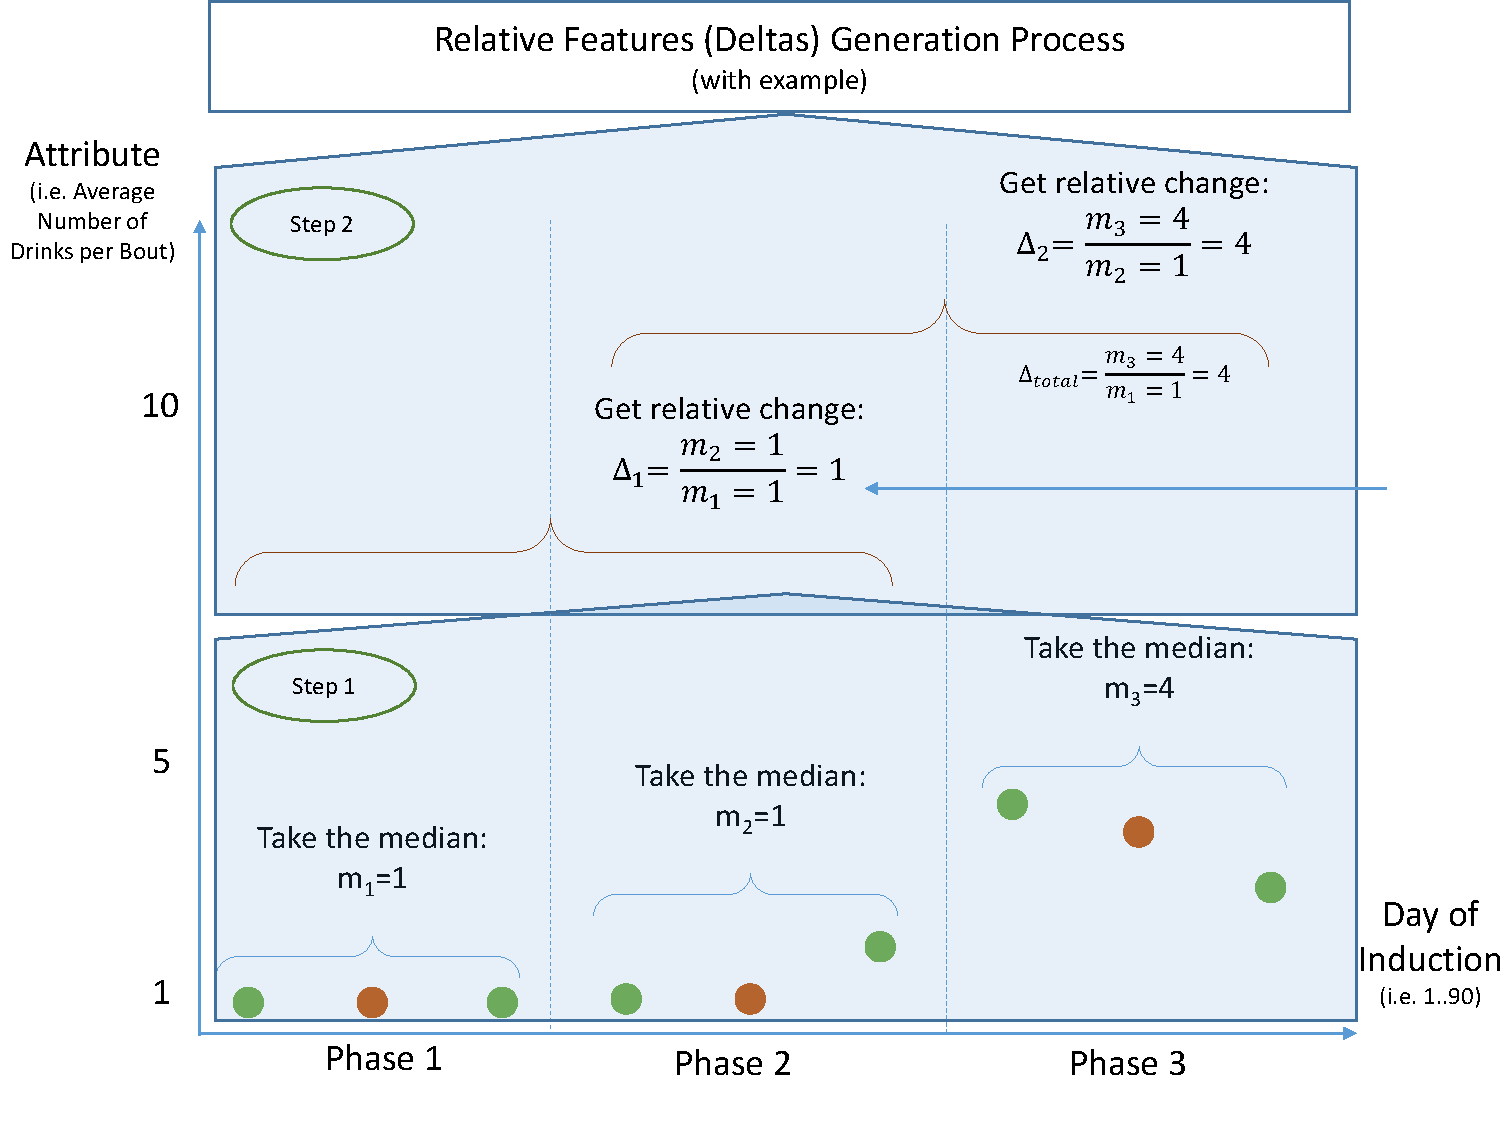
\includegraphics[width=1.1\linewidth]{figures/features_generation.pdf}
		\caption{Relative features (deltas) generation process.}
		\label{features_generation}
	\end{figure}
		
	The third step captures the tendencies of attribute values along the induction time-line. We decided to split 90 days into three stages (which relates to the three different dosage of total ethanol allotment for the day), and to take the central tendency value. Median was chosen because, unlike mean, it alleviates data inconsistency problems, described in the previous section. At the end of this step we had three absolute values for each attribute. We could not compare these values yet, because they \textit{do not indicate the changes in the drinking behavior} of the animal.
	
	The last step makes values comparable by converting absolute values to relative values as formally presented in formula \ref{eq:rel-deltas}. For each attribute, the median of the second stage is divided by the first and median of the third stage is divided by the second yielding two \textbf{relative deltas }, showing by \textit{how much, relatively, an animal changed its alcohol consumption preferences over the course of induction.} 
	
	\begin{equation} \label{eq:rel-deltas}
	\Delta_{ij}^{attr}=\frac{Median(atrr_{stage_i})}{Median(atrr_{stage_j})}, \text{where } i,j=1..3, j \neq j
	\end{equation}
	
	By performing these four steps we created comparable relative deltas that capture changes in the drinking behavior. Consider the example shown in the Figure~\ref{features_generation}: $\Delta_1=1$ indicates no change in behavior regarding this attribute, $\Delta_2=4$ indicates a four-fold increase in preference, which is comparable to the increase by other animals. On the other hand, if all the animals consumed their allotments in the first drink, on average, due to the small size of the allotment, this generated feature (delta) would not show any significance, because each animal would have same value of 1.

	\subsection{Feature Selection \label{section:feature-selection}}
	In addition to good features, machine learning algorithms require an appropriate number of features. Having too many features, especially \textit{if the number of features exceeds the number of observations (n), usually leads to ill-posed models and underdetermined mathematical solutions}. Failure to reduce the dimensionality of the problem by limiting the feature set to those with the highest predictive power can prevent systems from adequately determining which features augment, counteract, or contribute to the eventual outcome \shortcite{barber2012bayesian}.
	
	A forward selection strategy, which we employed in this study to select the most appropriate features, tests a model iteratively, increasing the number of features at each iteration and measuring the accuracy using a K-fold cross-validation \shortcite{alpaydin2014introduction}. Each forward selection iteration adds the feature that gives the best increase in performance in combination with existing features already in a set of chosen features. 

	\subsection{Novelty Two-Step Classification Model}	
	\begin{table}[h]
		\centering
		\caption{Drinking category distribution in cohorts. }
		\label{tab:dc-by-cohort}
		\begin{tabular}{llllll}
			\hline
			\abovespace\belowspace
			Cohort & Sex & LD & BD & HD & VHD\\
			\hline
			Rhesus 4  & M & 5 & 4 & 1 & 0 \\
			Rhesus 5  & M & 0 & 1 & 3 & 4 \\
			Rhesus 6a & F & 0 & 0 & 0 & 6\\
			Rhesus 6b & F & 3 & 9 & 1 & 1\\
			Rhesus 7a & M & 3 & 1 & 2 & 2\\
			Rhesus 7b & M & 3 & 1 & 1 & 0\\
			Rhesus 10 & M & 2 & 3 & 1 & 2\\
			\hline
		\end{tabular}
	\end{table}
	
	Having multiple categories and few observations leads to underdetermined solutions and ill-posed models of classification. Unless we are interested in detection rather than classification, an ideal classification framework contains a larger number of observations than categories and uniform observations within each category. Since the work presented here does not fall into that ideal framework (four categories, 50 observations, and inconsistent observations per category, see Table~\ref{tab:dc-by-cohort}) we reduce the number of categories from four to two and implement a two-step classification process. The first step distinguishes between two combined groups of similar categories: (1) LD and BD, and (2) HD and VHD. The second step differentiates the categories within groups separately. That is, LD and BD are now separated and classified individually as subcategories of the original group, and HD and VHD are also separated and classified individually using different parameters for each classification subgroup. Choosing different parameters for subcategories allows us to reduce the dimensionality of the problem and retrieve misclassified animals by identifying different behavioral aspects. 
	
	\subsection{Performance Measure \label{section:performance-measure}}
	Typically, standard accuracy is the way of measuring performance in ordinary classification problems, which is computed as the total number of correctly classified samples over the total number of samples. Additionally, our accuracy rate is modified to allow for a two-step classification model. The accuracy, thus, is computed by multiplying the prior probability of a sample being in a group (LD \& BD or HD \& VHD) by the standard accuracy in either of those two groups. Composite accuracy is then computed by multiplication with standard accuracy of the first step classification. Accuracy is always computed using a 10-fold cross-validation strategy that was averaged across 20 runs. 
	
	The base rate is used to determine how well the proposed methodology performs comparatively with the naive approach. Here, the base rate is defined as follows: let $D$ be the list of ''targets", or the list of categories corresponding to each observation in the training data; let $g(D,c)$ be a function over the list of targets, with the count of items in the list $D$ that are equal to category $c$. Given an observation of the data, $x$, we define our base rate as a naive classifier: 
	\begin{equation} 
	NaiveClassifier(x)= \argmax_{c}g(D, c) \label{eq:naive-classifier}
	\end{equation}
	A naive classifier in equation \ref{eq:naive-classifier} is not a poor classifier, but rather an educated guess that chooses the category with strictly the greatest number of occurrences. This naive classifier is better than choosing at random with no prior information of the data.



	\chapter{Results}
The primary motivation for this research is to learn more about alcoholism, its causes, accompanying characteristics and consequences. In our effort we conducted multiple studies, each taking advantage of a different, uniquely suitable set of tools. We trace their effectiveness, validity and limitations in achieving the thesis objectives of:
\begin{itemize}
	\item describing data in meaningful visual form;
	\item aligning and cross examination of data of different sources;
	\item generating hypothesis;
	\item observing gender and drinking category differences;
	\item understanding the predictive power of the alcohol induction data on the future levels of alcoholism.
\end{itemize}

The chapter describes our major studies and their results, presented in two separate sections. The first section describes five separate investigations aimed at quickly discovering and testing new hypothesis. We found that using Django ORM and Python's SciPy ecosystem greatly facilitates that task. Using various analytical tools, described in detail below, we demonstrate the following findings: 
\begin{itemize}
	\item Animals increase their need for fluid after they eat. Heavy drinking animals appear to have a preference of alcohol over the water resulting in peaks in alcohol consumption after the food intake. 
	\item Drink-to-bout ratio is a good indicator of habitual drinking. KDE plot reveals a divergence of habitual drinking between females when the periods of first nine months versus last three months are considered. This is not the case for males.
	\item Menstrual cycle strongly affects alcohol consumption in females. Peaks in ethanol drinking follows the peaks of progesterone levels with the lag of few days. Females appear to drink more alcohol in their post-luni phase of the menstrual cycle.
	\item Binge drinking animal have a sporadic drinking pattern. Low and binge drinkers are averse of drinking on the day after intoxication. On contrast, heavy drinkers appear to tolerate intoxication well, which, on the other hand, may indicate the innate inability to quit drinking. 
	\item Heavy drinking females reduce their alcohol consumption much less the day
	after intoxication than low drinking ones; conversely, heavy drinking males reduce
	their drinking more the day after intoxication than low drinking ones.
\end{itemize}

The second section describes the detailed study of the prediction of future levels of alcoholism based on the early (induction) drinking and behavioral data using machine learning techniques. Our main contributions are in creating new attributes, generating relative feature reflective of adaptation process, adjusting Random Forests model and developing novel two-step classification model. 

\section{Discovering and Testing New Hypothesis}
	Given the large volumes of data describing each sample, it is desirable to produce new hypothesis with regard of the general population. Slicing and aggregating data by new angles and visualizing it gives us opportunity to identify anomalies or tendencies and make a hypothesis. Additionally, employees that work with the animals directly notice peculiarities in the animal behavior, which may lead to apriori knowledge. A biologist can infer what the causes of that might be, and a data analyst can test hypothesis given the appropriate data is present. 	
	
\pagebreak	
	\subsection{Drinking Pattern}
	Recall that during the open access phase of the experiment, concurrent access to water and alcohol solution is available to the subjects. Each day's session lasts 22 hours, which guarantees at least two hours of no alcohol for heavy drinkers. At the end of the eighth hour of the session the lights in the cages are turned off; at the beginning of the 20th hour the lights are turned on. Food pellets are available on demand in specified intervals during the day, starting at hour zero. 
	
	One objective is to determine whether or not the drinking patterns of low drinkers differ significantly from that of heavy drinkers. To answer this question we needed a visual representation of alcohol consumption during the day by each animal. The problem is that the drinking varies from day to day, and we need to see ``averaged" picture. 
	
	In the database we store raw data about alcohol drinks (defined as drinking without stop for more than five seconds) during the day by each subject. Each drink is a row with the values for drink start time, drink stop time and the amount consumed. To produce the ``average" drinking pattern for each animal we retrieve the data about the drinks and current weight, and then apply the algorithm~\ref{alg:cum-drink-pattern}:
	
	\begin{algorithm}[H]	%TODO better package for algorithm	
		%\KwData{this text}
		%\KwResult{how to write algorithm with \LaTeX2e }
		%initialization\;
		1. \ForEach{Session}{
			1.1. Get the list of drink as tuples (volume, end time)\; 
			1.2. Replace each tuple's volume with EtOH (g/kg) = volume / animal.weight\;
			1.3. Sort the list by ``end time"\;
		}
		2. Merge each session's list of tuples into one long list\;
		3. Sort the list by ``end time"\;
		4. Apply cumulative sum operation on the EtOH (g/kg) in the list\;
		5. Divide all EtOH (g/kg) by the total number of sessions.
	\caption{Calculating cumulative average drinking pattern.}
	\label{alg:cum-drink-pattern}
	\end{algorithm}
	
	\begin{figure}[ht]
		\centering
		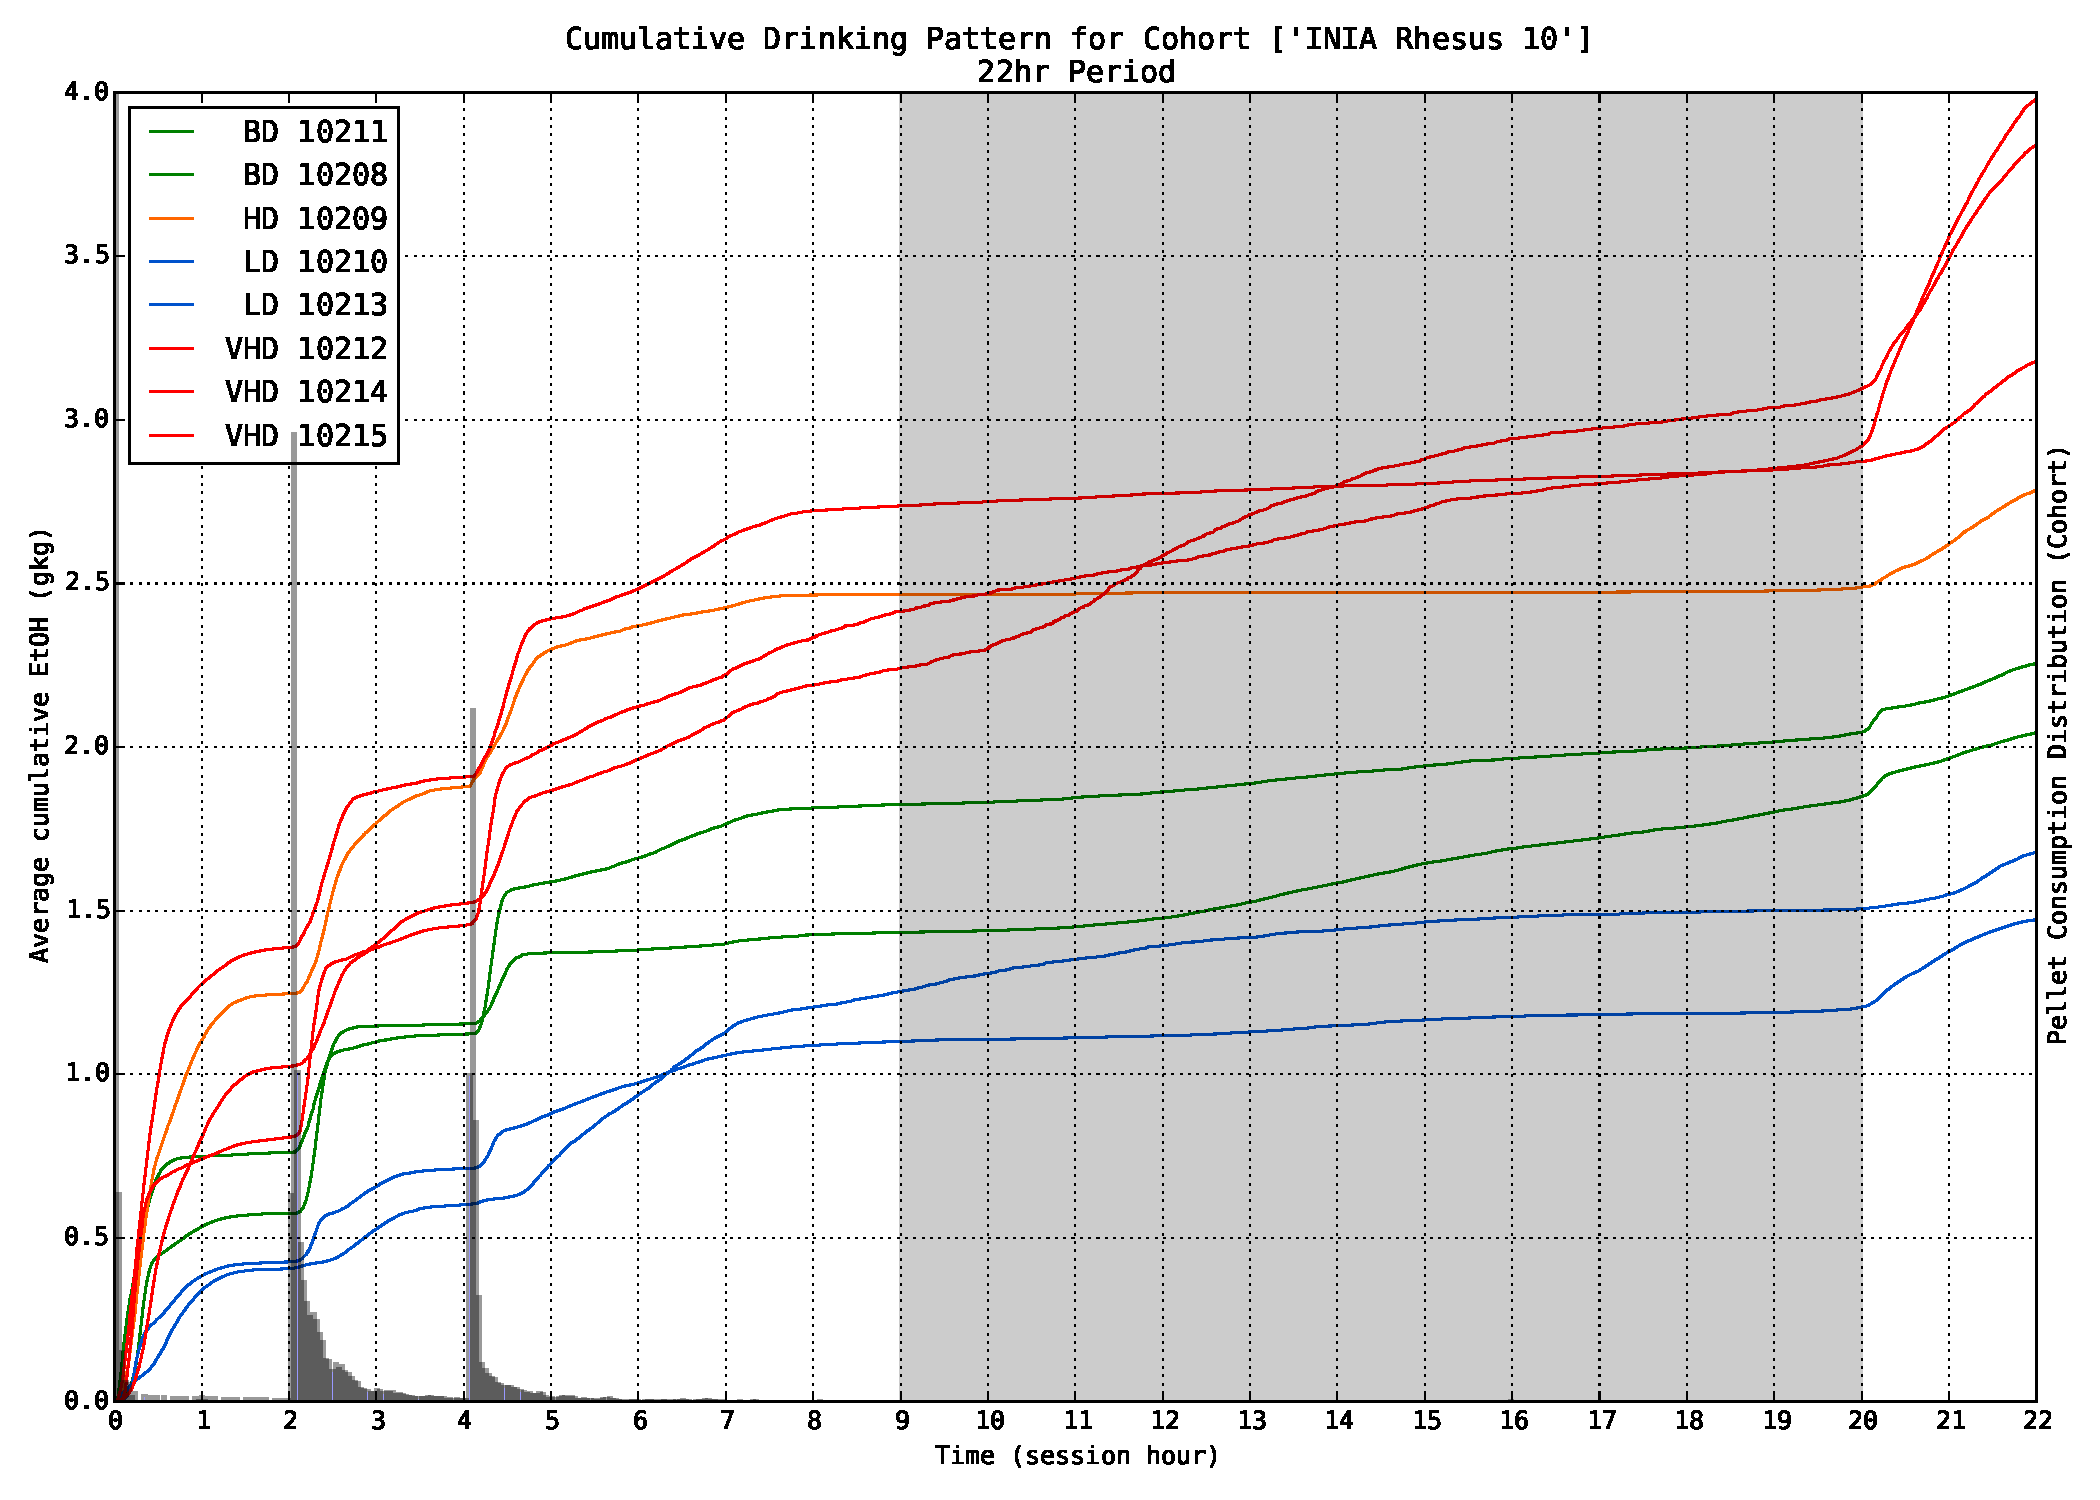
\includegraphics[width=\linewidth]{figures/dp_r10_m_22hr.pdf}
		\caption{Cumulative average drinking pattern plot for 22 hour session. Dark area depicts when lights were off in the cage. Lines show ethanol consumption for each animal. Histogram illustrates food pellet time distribution for the entire cohort.}
		\label{fig:dp-22hr}
	\end{figure}
		
	Algorithm~\ref{alg:cum-drink-pattern} produces normalized cumulative average drinking patter for each animal. The visual representation of the output of the algorithm for cohort ``INIA Rhesus 10" is shown in Figure~\ref{fig:dp-22hr}. The picture has peculiar distinct ``steps" in the lines of cumulative alcohol consumption. In an attempt to explain such phenomena we added food pellet distribution for the entire cohort in form of the histogram. Notably, while drinking patterns do not seem to be different for animals of different drinking category, food consumption has strong influence on alcohol consumption. This may be attributed to the fact that animals typically need fluid after they eat, regardless of what fluid might be. Low drinking animals may prefer water while heavy drinkers prefer the solution of 
	%sugary 
	water with alcohol. Overall, however, all animals drink more alcohol after they eat. 
	
	Another idea for improvement came from the lab employees. They noticed that animals started to drink alcohol as soon as staff appeared in the lab and before the lights actually turned on. Thus we decided to combine the data from the last two hours of the previous day with the current day. We noticed that there is not much activity during the lights off phase, thus used only first nine hours of the current day. Additionally, we de-trended each line of alcohol consumption by subtracting values of the linear regression line, individually for each animal. The result, for cohort ``INIA Rhesus 6b" is presented on Figure~\ref{fig:dp-dl}. Notably, low drinkers have much flatter lines then heavy drinkers who boost their alcohol consumption after the food pellet intake. The early noise does not appear to correlate with drinking behavior, however. 
	
	\begin{figure}[ht]		
		\centering
		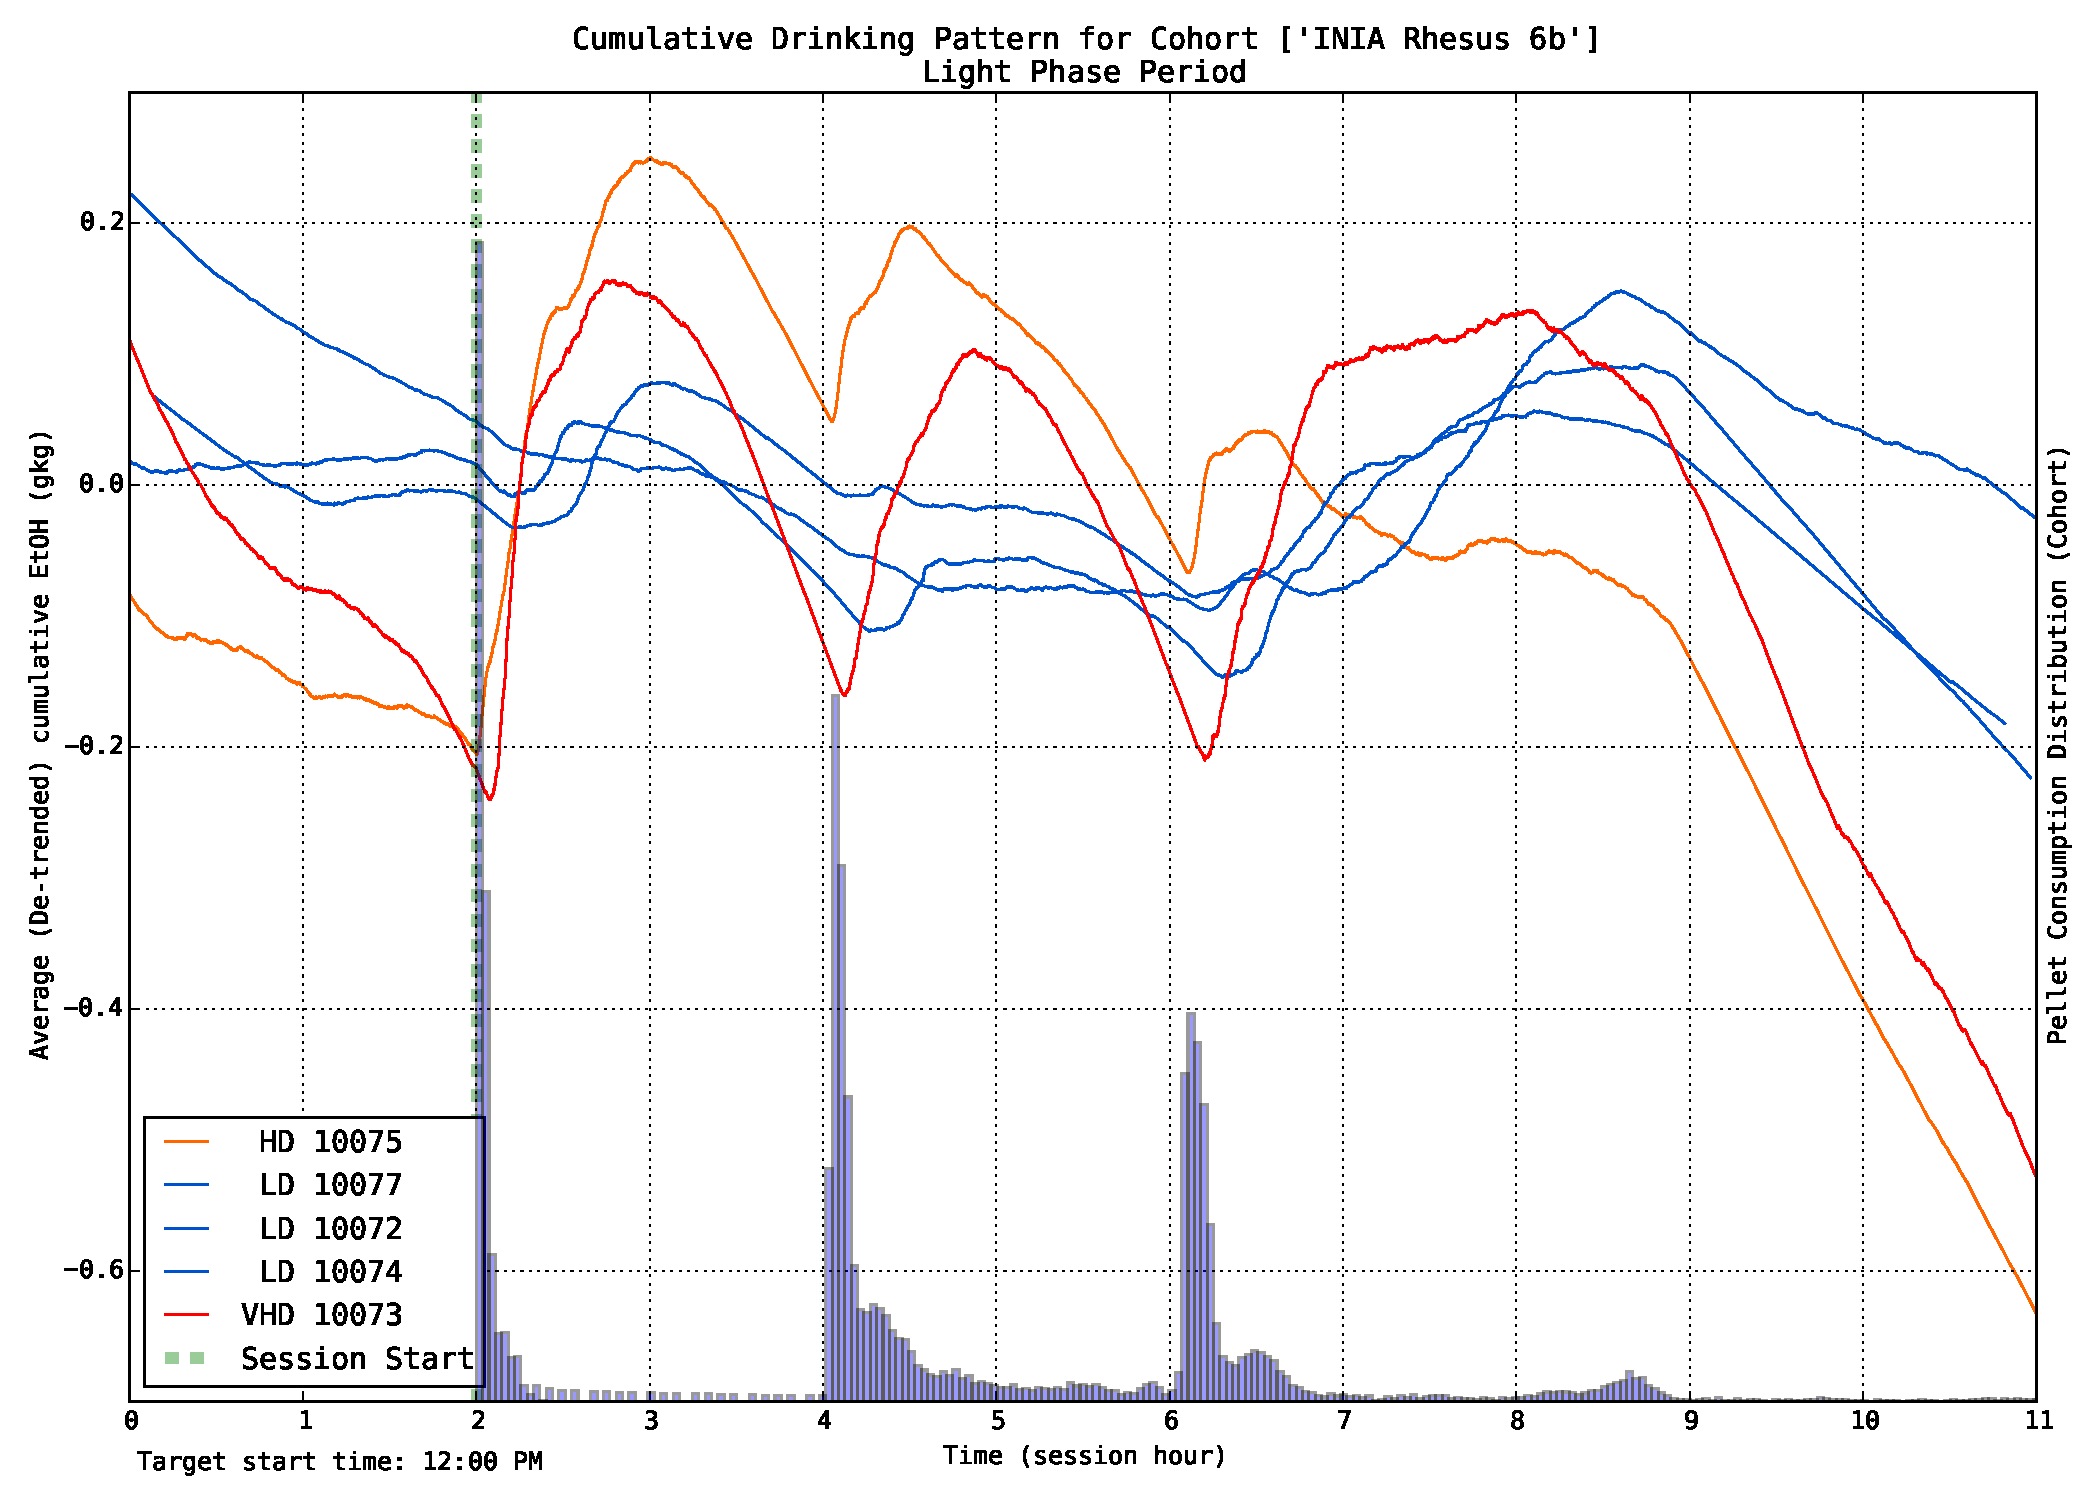
\includegraphics[width=0.98\linewidth]{figures/dp_r6b_f_lights.pdf}
		\caption{Cumulative (de-trended) average drinking pattern plot for daylight session, which includes two hours of the previous day plus nine hours of the current day. Lines illustrate (de-trended) ethanol consumption for each animal. Trend was calculated individually for each animal via linear regression of the first order. Histogram shows food pellet time distribution for the entire cohort.}
		\label{fig:dp-dl}
	\end{figure}
	
		
	\subsection{Habitual Drinking}
	The motivation for the habitual drinking study is to see if there are the differences between males and females in how their drinking habits change from the first nine months to the last three months of the open access. To capture \textit{habitual} drinking we observe the relationship between the mean drink length and the mean bout length. Thus a new daily attribute \textit{``drink-bout ratio"} is created. Factor boxplots can be used to compare between genders, drinking categories and time period, as shown in Figure~\ref{fig:habitual-boxplots-mf}. Such boxplots were created for each available attribute and for each drinking category. Looking through such boxplots allows us to generate new hypothesis.
	
	\begin{figure}[ht]
		\centering
		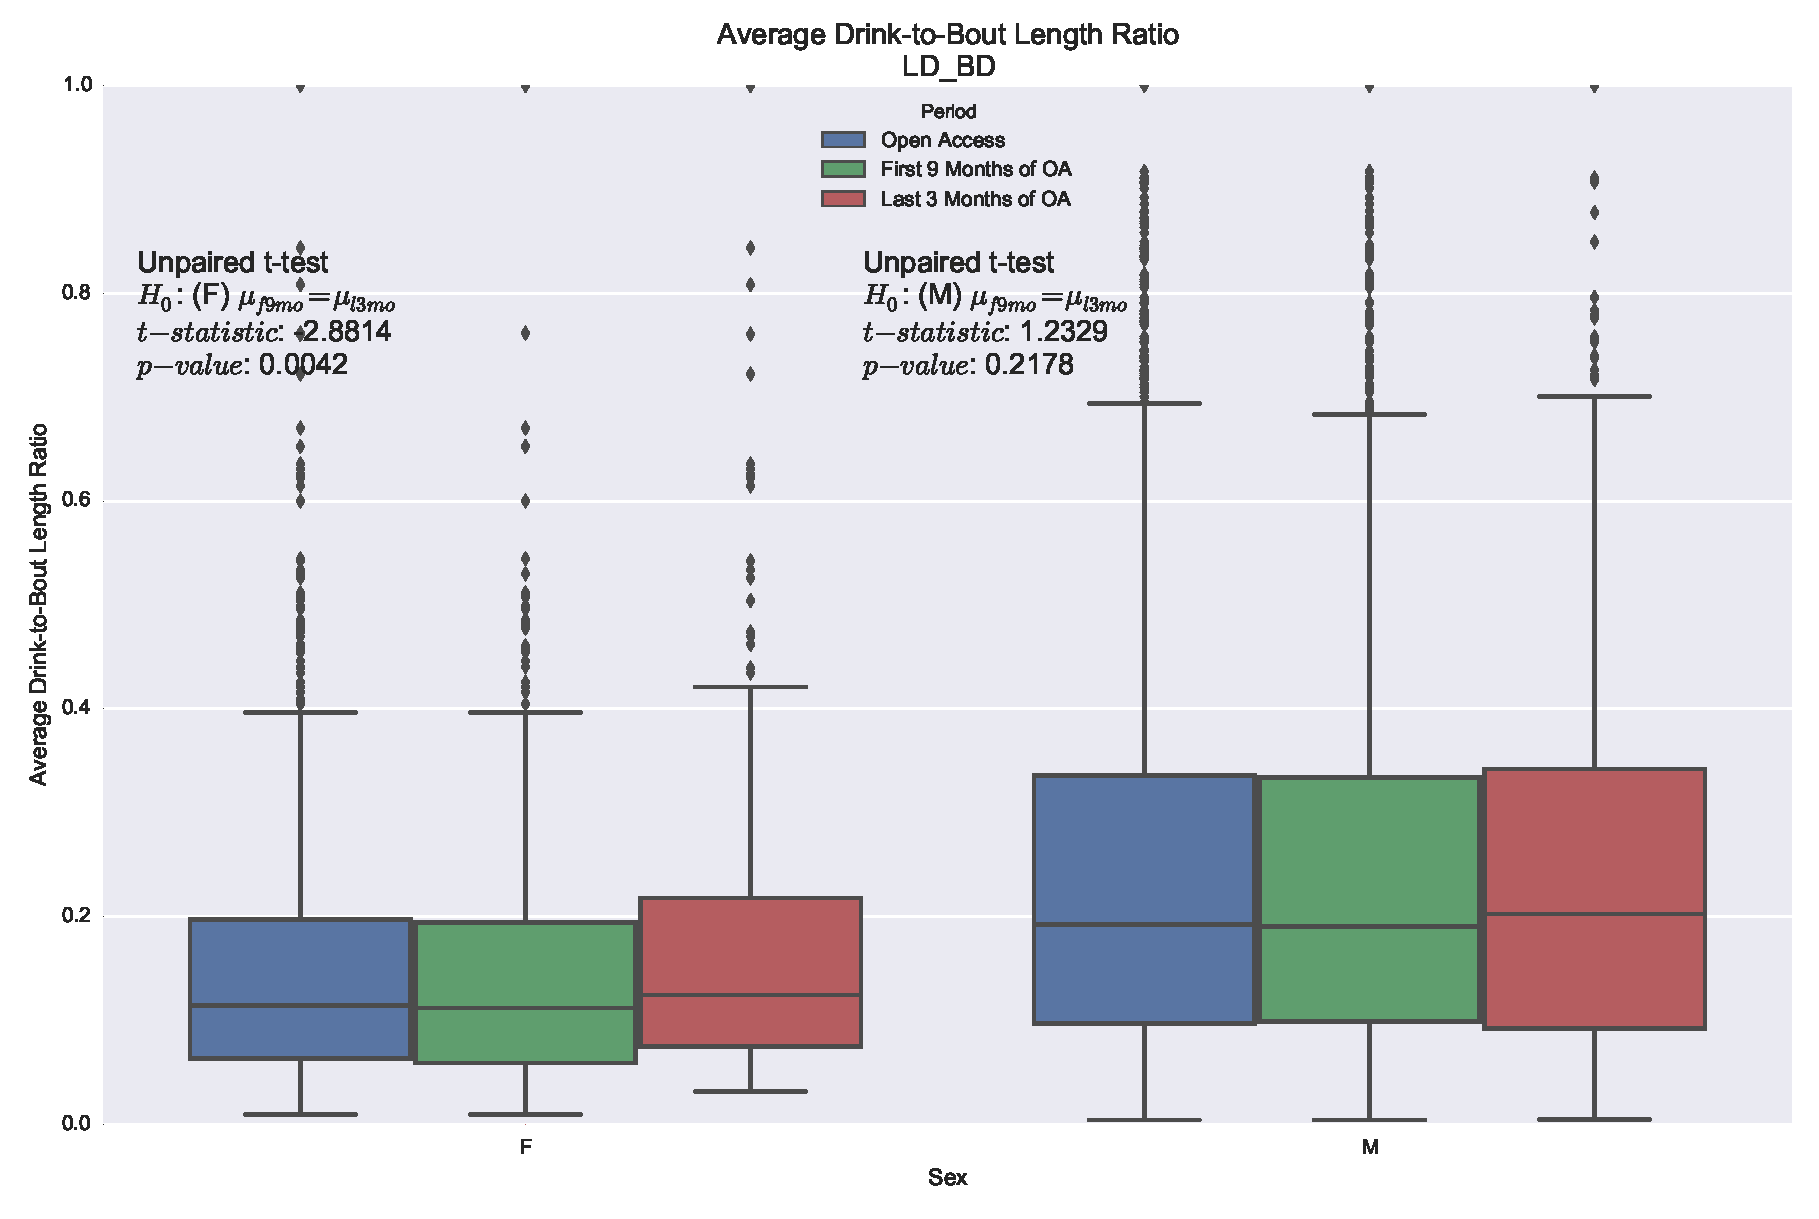
\includegraphics[width=1.1\linewidth]{figures/habitual_boxplots_mf_ttest.pdf}
		\caption{Habitual drinking factor boxplot shows the change in daily average ``drink-bout ratio" (green to red; blue - total) in both male and female populations. A t-test is used to check statistical significance of  changes.}
		\label{fig:habitual-boxplots-mf}
	\end{figure}
	
	Figure~\ref{fig:habitual-boxplots-mf}, created for low and binge drinking animals (LD \& BD), contains additional information about unpaired t-test to test the hypothesis of whether the mean value of ``drink-bout ratio" is equal for the first nine months and the last three months of the OA. There is a significant statistical difference for females but not males. In the heavy and very heavy drinking animals (HD \& VHD) the picture is reversed: there is difference in males but not females.	
	
	\begin{figure}[ht]
		\centering
		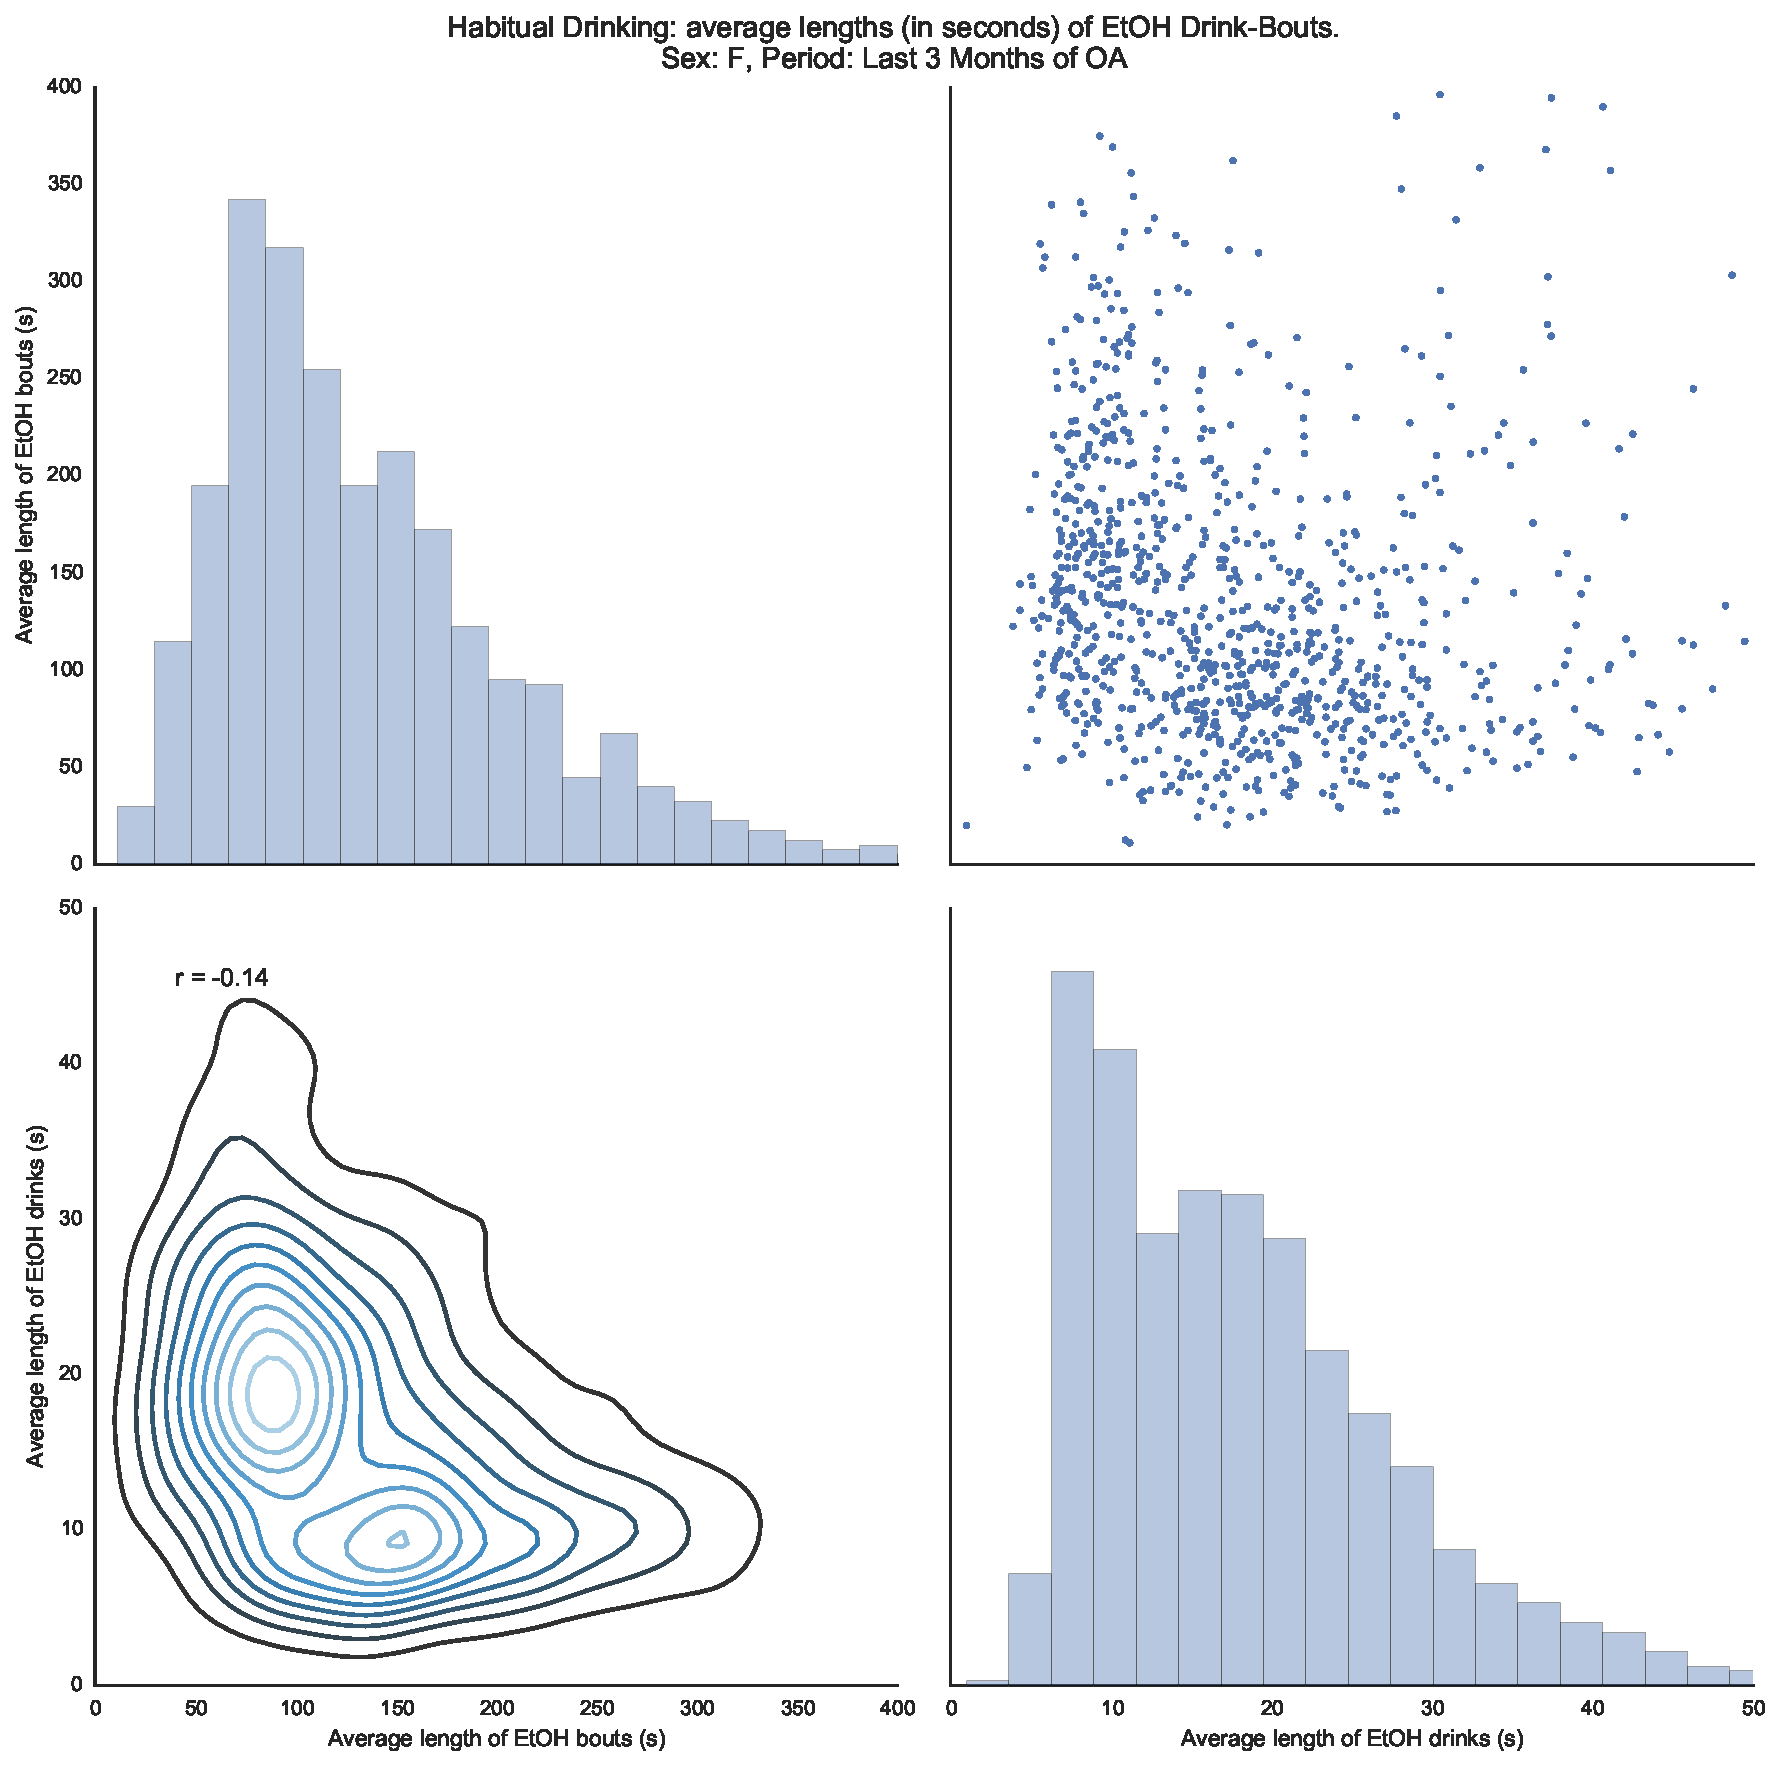
\includegraphics[width=0.85\linewidth]{figures/habitual_f_l3mo.pdf}
		\caption{Habitual drinking pair plot of the last three months of open access period for females. The X-axis represents daily average length of ethanol bouts in seconds; Y-axis shows daily average ethanol bout length. Histograms of both attributes are present on the diagonal. In the upper right corner is the scatterplot of data points for each animal per drinking day. In the lower left corner is the same data shown as a KDE plot.}
		\label{fig:habitual-l3mo-f}
	\end{figure}
	
	After we confirmed that ``drink-bout ratio" helps explain variation in the data, we decided to explore that attribute further. A pairplot captures the relationship between drinks and bouts precisely, as shown in Figure~\ref{fig:habitual-l3mo-f}. As with the boxplots, figures were created for each gender, drinking category and time period, allowing us to track data differences visually.  
	
	Figure~\ref{fig:habitual-l3mo-f} is a pairplot for female population during the last three month of OA. While histograms for each attribute show the anticipated distribution, the main diagonal of the scatterplot appears to be more sparse than the zones along the axis. To facilitate better visual perception, KDE smoothing of the multiple data points is used to plot contours of this bivariate distribution. KDE plots reveal two modes\footnote{In statistics, modes are the most frequently occuring values.} in the drink-to-bout relationship - a characteristic that is not initially (first nine months of OA) present in females and not present in males at all. 	


	
	\subsection{Menstrual Cycle Affecting Alcohol Consumption \label{section:mense}}
	The next study demonstrates how aligning and correlating data from different sources can show complex reoccurring characteristics of primate drinking, namely how the menstrual cycle affects alcohol consumption in female population. The base of the Figure~\ref{fig:mense} is a scatterplot (green dots) of the daily total ethanol intake (primary left Y-axis) during open access for one animal. To improve visual perception of the ethanol intake and to see the trend by smoothing the oscillation we applied the locally weighted linear regression technique (resulted in the green line), as explained in \cref{lwlr}. Additionally, days of the menstruation are shown with the transparent vertical red rectangles.
	
	Progesterone is a sex hormone involved in the menstrual cycle, pregnancy, and embryogenesis of humans and other species \shortcite{king2010pharmacology}. The level of progesterone in blood was measured every two to four days in female cohort ``6a". These values are plotted as dots connected by lines on top of the basis layer with secondary (right) Y-axis indicating the exact amount. The correlation between the hormone level and smoothed drinking osculations is now accessible by the naked eye: this heavy drinking female is drinking notably more a few days after peak progesterone.   
	
	\begin{figure}[ht]
		\makebox[\textwidth][c]{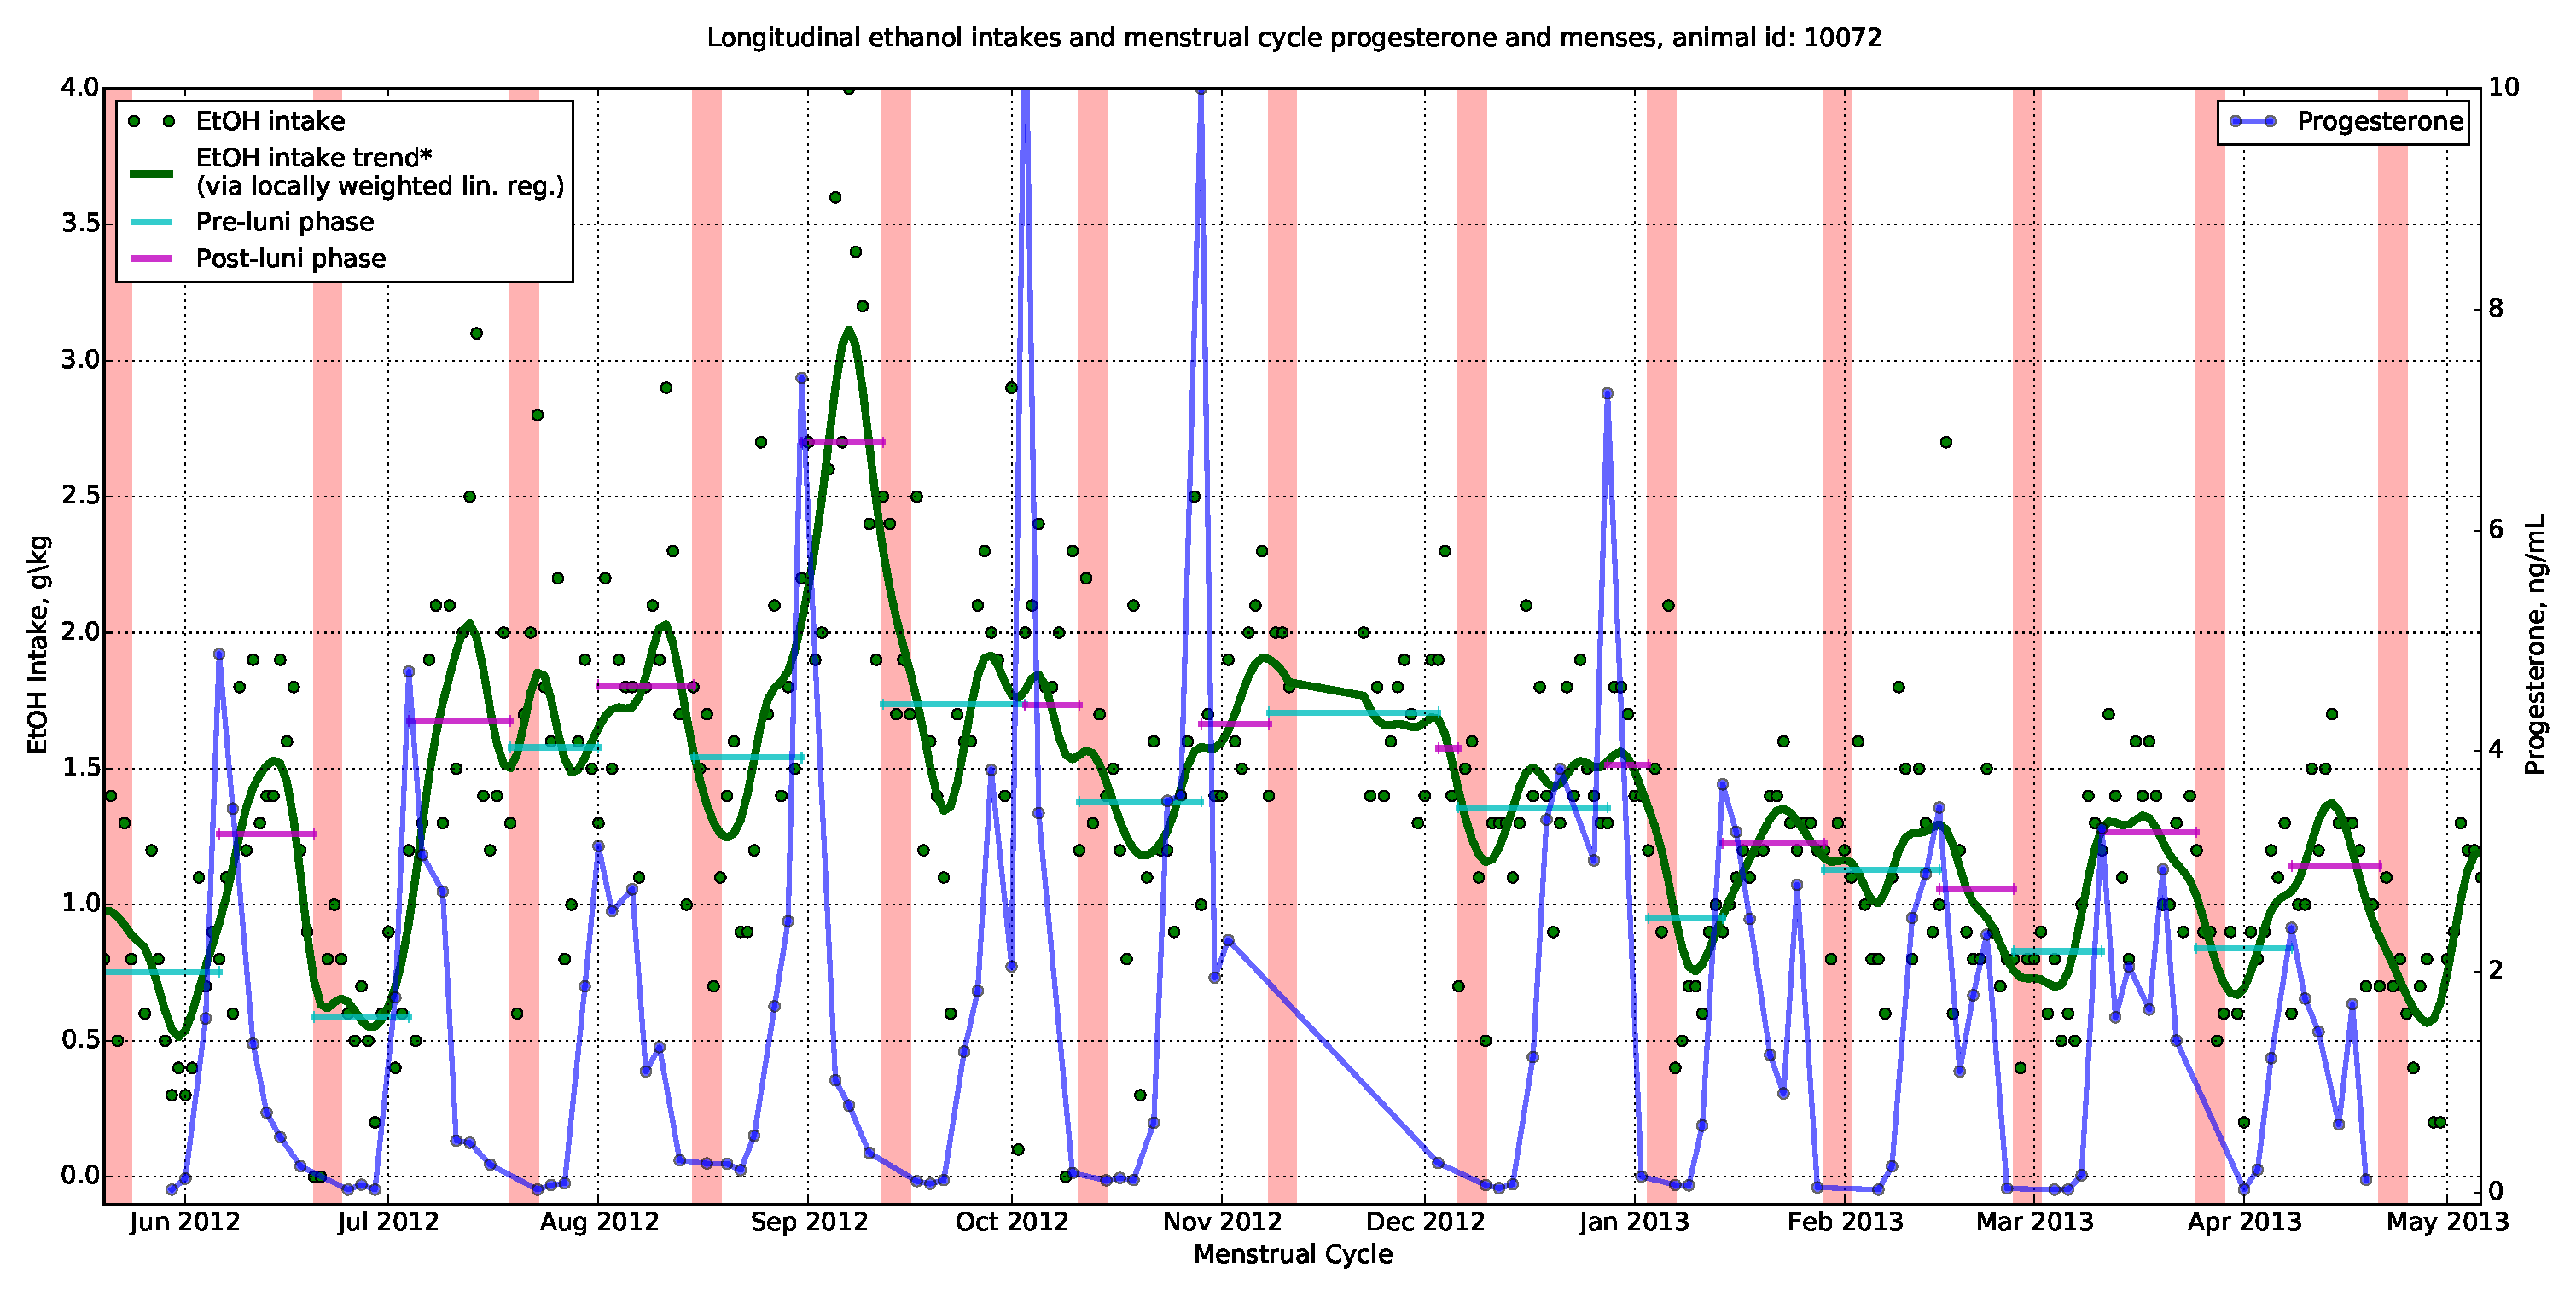
\includegraphics[width=1.3\textwidth]{figures/mense_progesterone_oa.pdf}}
		%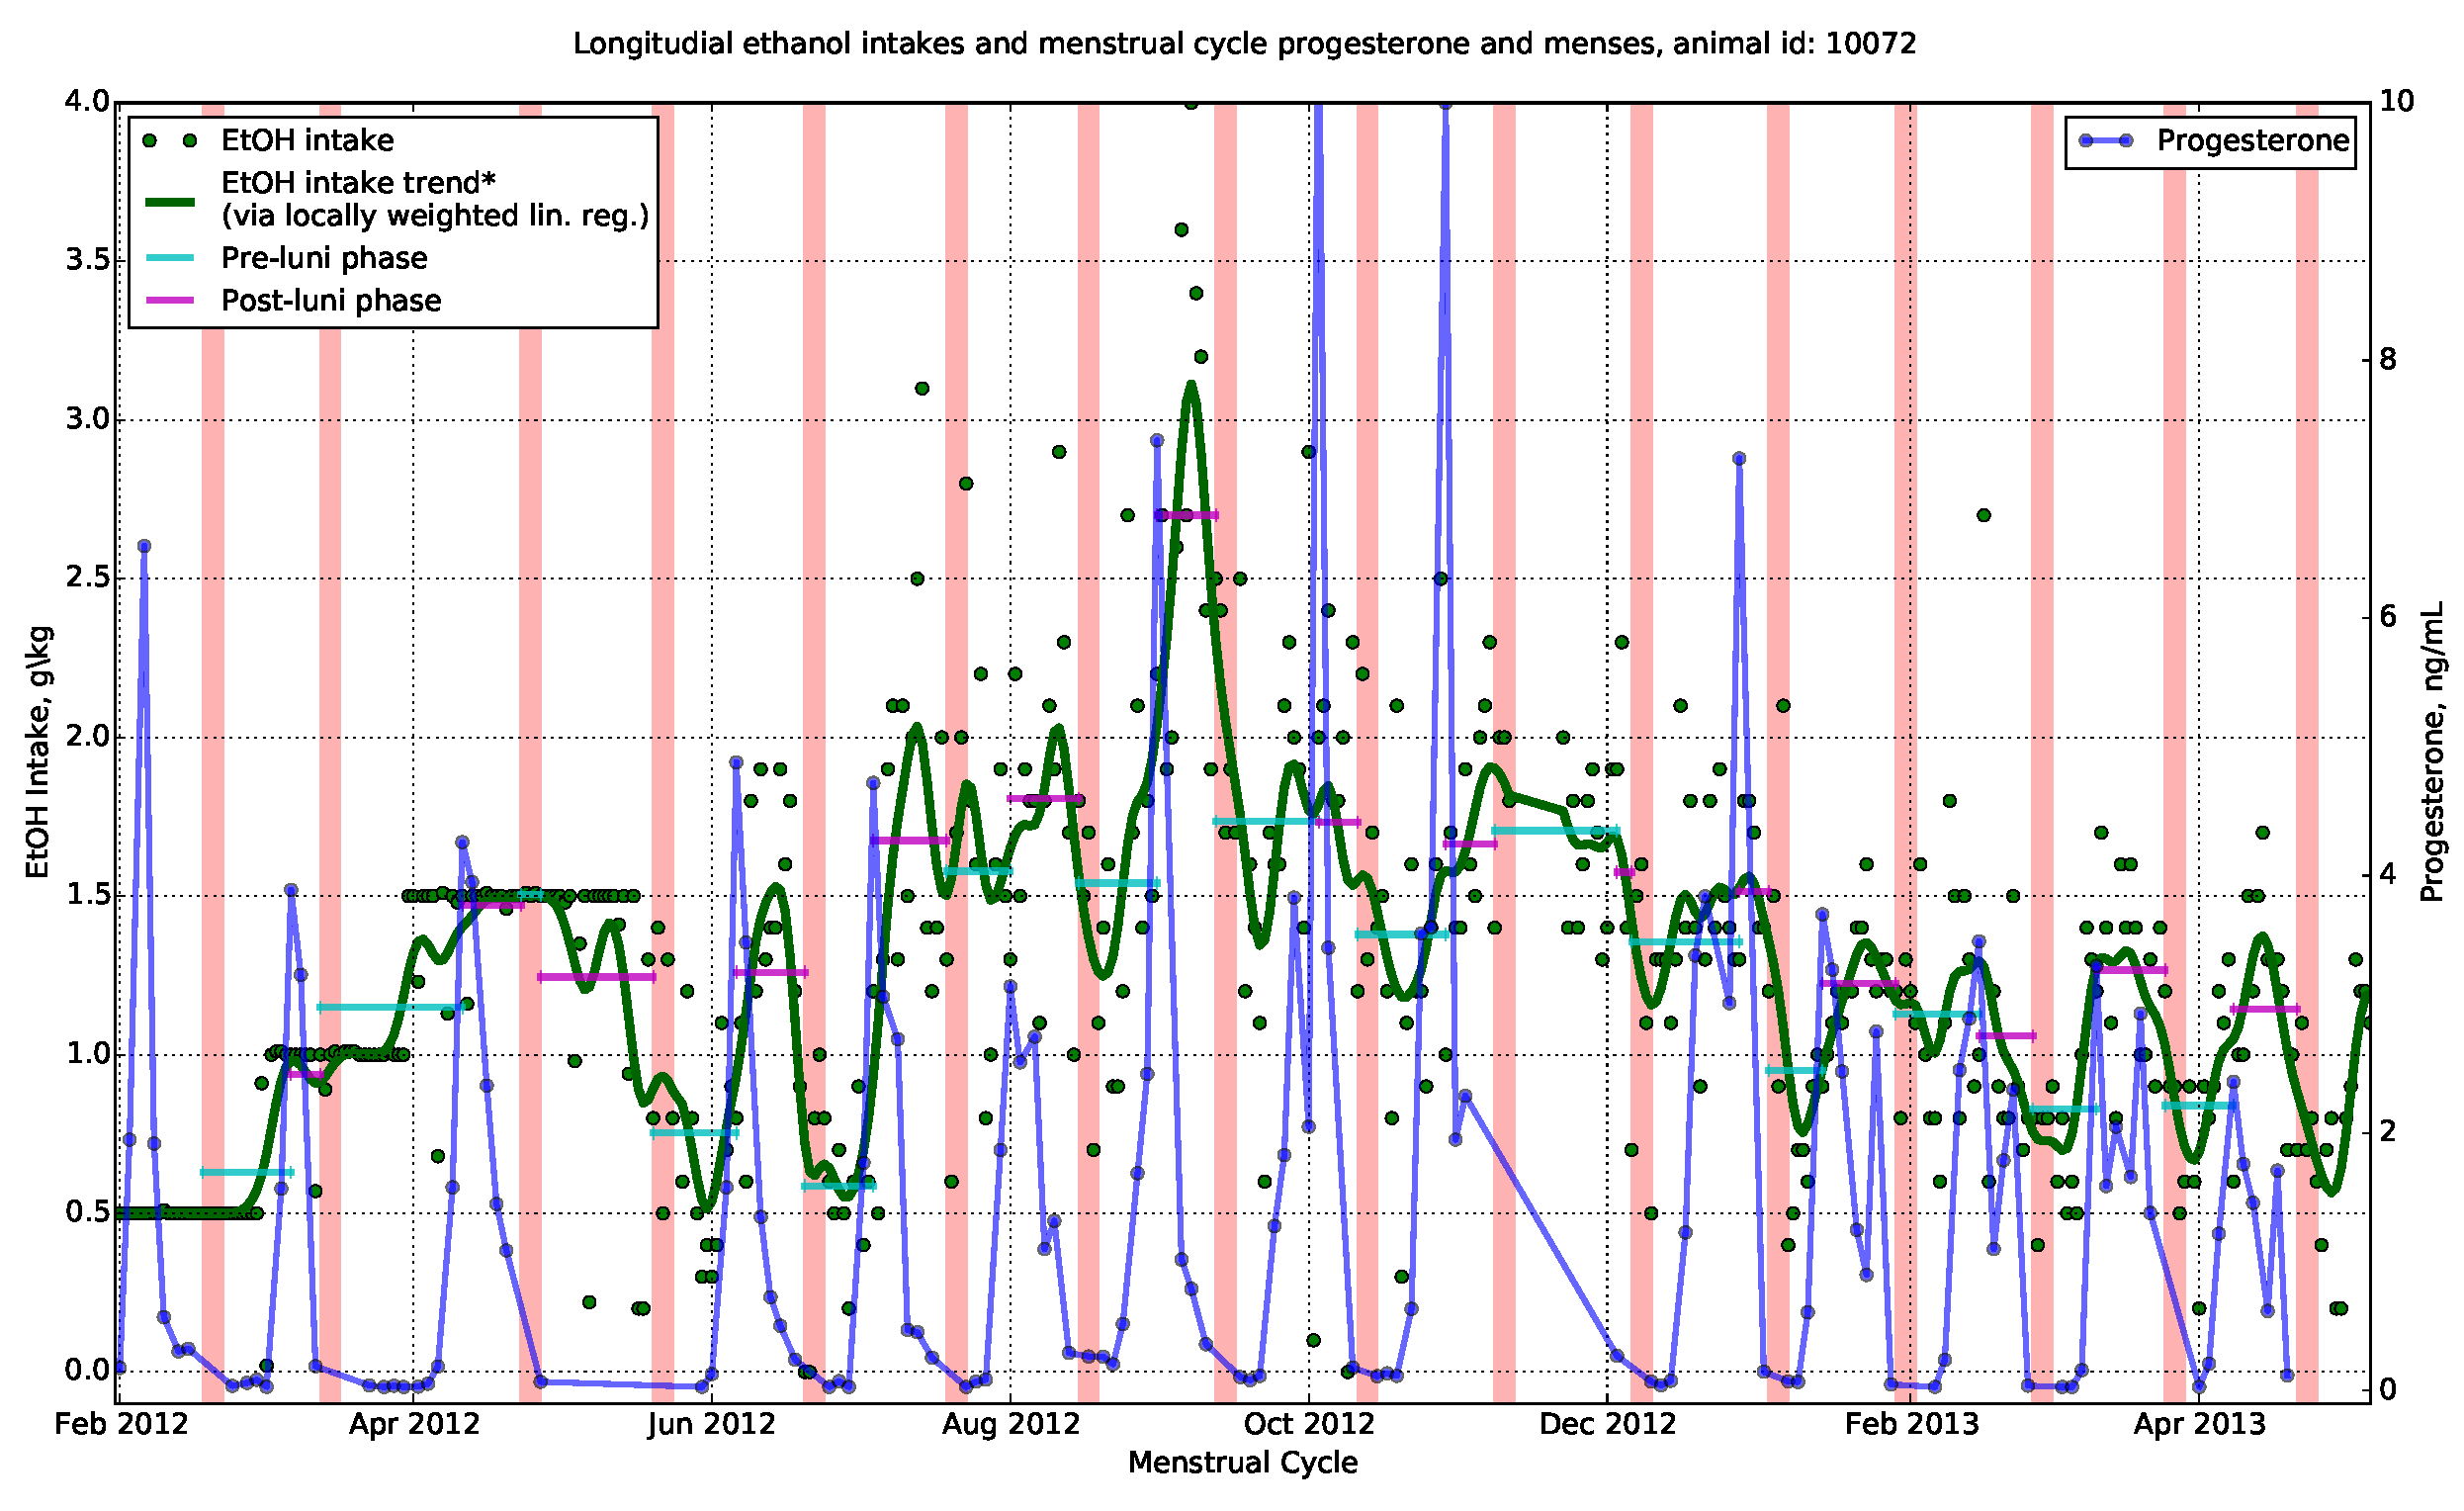
\includegraphics[width=1.3\linewidth]{figures/mense_progesterone.pdf}
		\caption{Menstruation cycle influence on ethanol intake. Vertical red rectangles depict days of  menstruation by date in the X-axis. Dots represent daily EtOH consumed as average in g/kg. The green line shows the smoothed trend obtained via locally weighted linear regression; the blue line connects the points of progesterone level observations. There is a visual correlation between green and blue lines. Cyan and purple horizontal lines show pre-luni and post-luni menstrual phases, respectively.}
		\label{fig:mense}
	\end{figure}
	
	To extend the analysis of how much this animal's drinking changes, on average, we first divide all the ethanol intake data points by full menstrual cycle. Then, within each cycle, we divide data points into two phases: pre-luni and post-luni. Pre-luni phase starts with the beginning of the cycle and ends when the progesterone level is in the highest (peak in the blue line). Post-luni begins here and ends with the start of new cycle. For each pre-luni and post-luni phase within each cycle the average ethanol intake was calculated and plotted as a horizontal lines (cyan and purple colors, respectively). In every case but one the level of average ethanol intake is much higher during the post-luni phase then during the pre-luni phase which indicates the direct influence of female hormones on the alcohol consumption. 
	

	\subsection{BEC $\sim$ EtOH Correlation}	
	Throughout the ethanol self-administration experiment there were regular (every fifth day) blood drawings  that track the Blood Ethanol Concentration (BEC) levels in the subjects. The BEC is an objective measurement of intoxication. However, there are some issues too: since blood is drawn only once every five days at an arbitrary time it may be the case that some animals, preferring morning drinking, are already getting sober, while others, preferring night drinking, have not yet started their alcohol consumption. Hence this study aims to investigate the reliability of the BEC as well as to look for anomalies and specific patterns. One particular pattern was watched for: do animals from different drinking categories drink differently the day after hard alcohol intoxication (defined as above a certain level of BEC)? Below is a description of the study along with the results, implications and limitations. 
	
	First, we gathered the BEC data from regular samples from available cohorts\footnote{Few cohorts do not provide BEC data.} resulting in nearly 6000 rows containing animal id, date and time of sample, and the BEC in form of milligram percentage (mg \%). Then the ethanol consumed up to the sample time that day was calculated for each animal (EtOH day of BEC sample). Then values for the total ethanol consumed the days before and after the BEC sample were retrieved (EtOH day before and EtOH day after, respectively); days with exceptions in either BEC or EtOH data were filtered out.
	
	\begin{figure}[ht]
		\centering
		\makebox[\textwidth][c]{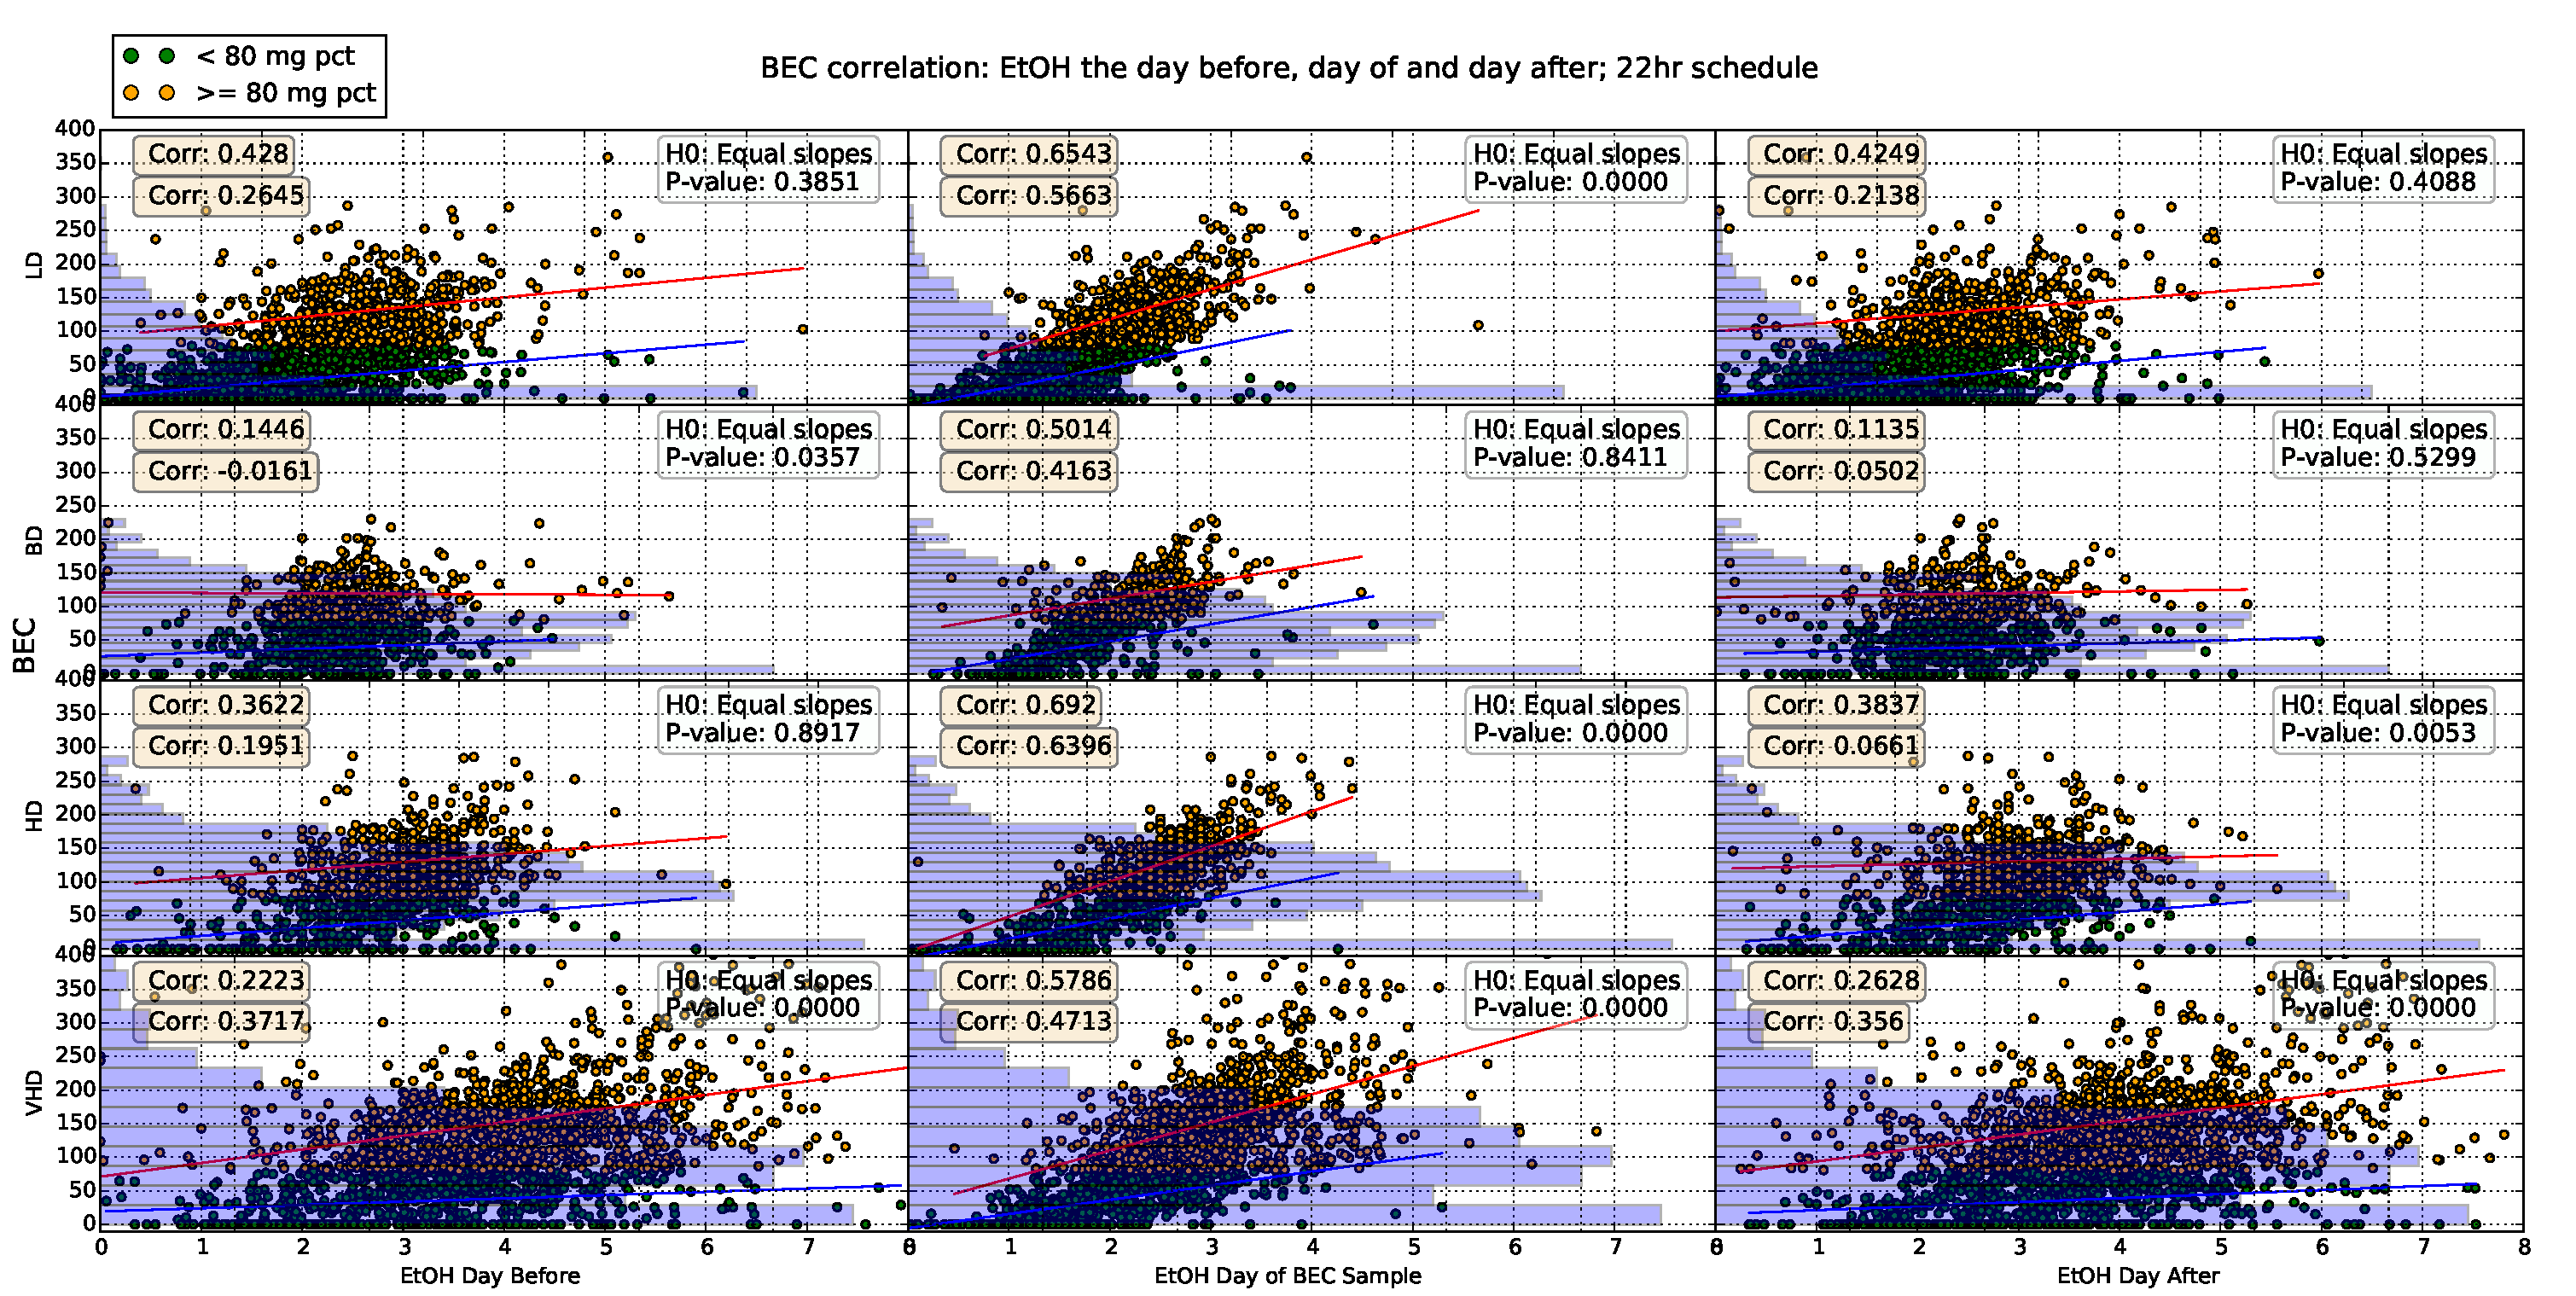
\includegraphics[width=1.2\textwidth]{figures/bec_etoh_over80mg_22hr.pdf}}
		\caption{Combined BEC $\sim$ EtOH correlation plot for all animals displaying a grid of panels: four rows by drinking category, three columns with ethanol the day before, the day of and the day after the BEC sample. On each panel Y-axis represents the level of BEC (mg \%) the day of sample. The X-axis represents the ethanol consumed by the animal: total EtOH the day before BEC sample in the left column, total EtOH up to the sample time at the middle column and total EtOH the day after BEC sample in the right column. Each panel describes the ethanol versus sample BEC, divided into two groups (less or more than 80 mg pct BEC) and contains: scatter plot of EtOH$\sim$ BEC; sample's BEC values overlaid as histogram (grouped by drinking category); Pearson correlation product for each group; linear regression fit lines and ANCOVA p-value testing whether those two lines have equal slopes.    }
		\label{fig:bec-over80}
	\end{figure}
	
	At this point we had approximately 5500 data points with the following information: animal id, drinking category, sample BEC level, EtOH day before, EtOH day of BEC sample and EtOH day after. Ultimately, we wanted to see and measure the correlation between ethanol consumed at one of the three consecutive days and BEC level at each slice of the qualitative attributes. Additionally, we wanted to see if the intoxication event plays a role and divided all data points into two groups: BEC at intoxication level equal or over 80 mg \% or not. 
	
	Visual representation of the results is shown on the Figure~\ref{fig:bec-over80} containing a grid of panels. Rows separate drinking categories and columns represent EtOH the day before, day of and day after the BEC sample. Each panel has a scatterplot of data points described above. Points of intoxication are shown in orange. Surprisingly, low drinking animals appear to have elevated numbers of intoxication events. In fact, \textit{it seems} they have the same number of the orange points as the heavy drinking animals. This is, however, due to the high density of points, which skews the visual perception. By looking at the overlaid normed histograms of the BEC values for each drinking category we can see that intoxication, as defined here, is much more likely among VHDs than LDs.   
		
	Each panel on Figure~\ref{fig:bec-over80} also contains a Pearson correlation value and linear regression fit lines for each group, as well as the ANCOVA p-value for the hypothesis testing whether those two lines have equal slopes. First consider low drinking animals. Statistically (ANCOVA p-value) two groups (intoxicated or not) have a different line of ethanol consumption up to the BEC sample time, while the day before and the day after two groups do not differ. In binge drinking animals, two groups drink differently during the day before intoxication, but not the day of and the day after the sample. That may be an indicator that in BDs there is a factor today that causes the occasional drink tomorrow. In heavy drinkers the pattern is reversed: two groups drink similarly the day before intoxication, but differently the day of and the day after. That may indicate that once intoxicated HDs can not stop drinking, hence such divergence. In very heavy drinkers, coherently with the interpretation of HDs, two groups drink differently all three consecutive days, which may indicate that for them the intoxication becomes a vicious cycle. 

	While defining intoxication as over 80 \% BEC is a widely accepted method, it has limitations. For example, the ANCOVA model implies the assumption that the covariate is independent of the treatment effects. In our case it is not entirely true since we split the data based on the BEC level. Additionally, it may seem unfair to call two animals from \textit{different drinking categories} intoxicated after achieving the \textit{same level of BEC}. The alternative is to define alcohol intoxication for the animal as an event of ethanol consumption over an arbitrary threshold number of standard deviations \textit{for that particular animal}. The later part of this study adopts this definition with the threshold equal two\footnote{We do not use the lower threshold because there are a lot of zero BEC measurements due to the various reasons.}. Thus for each animal the intoxication is defined as EtOH consumed is over two standard deviations above the mean:
	\begin{equation} \label{eq:intox-std}
	\mathbbm{1}{ \{x > \mu + 2*\hat{s}\}}
	\end{equation} 
	
	As shown on Figure~\ref{fig:bec-over80}, besides incorporating the new definition, we alleviate the problem of high density scatterplots by using hexagonal bin (hexbin) plots.
	\begin{figure}[ht]
		\centering
		\makebox[\textwidth][c]{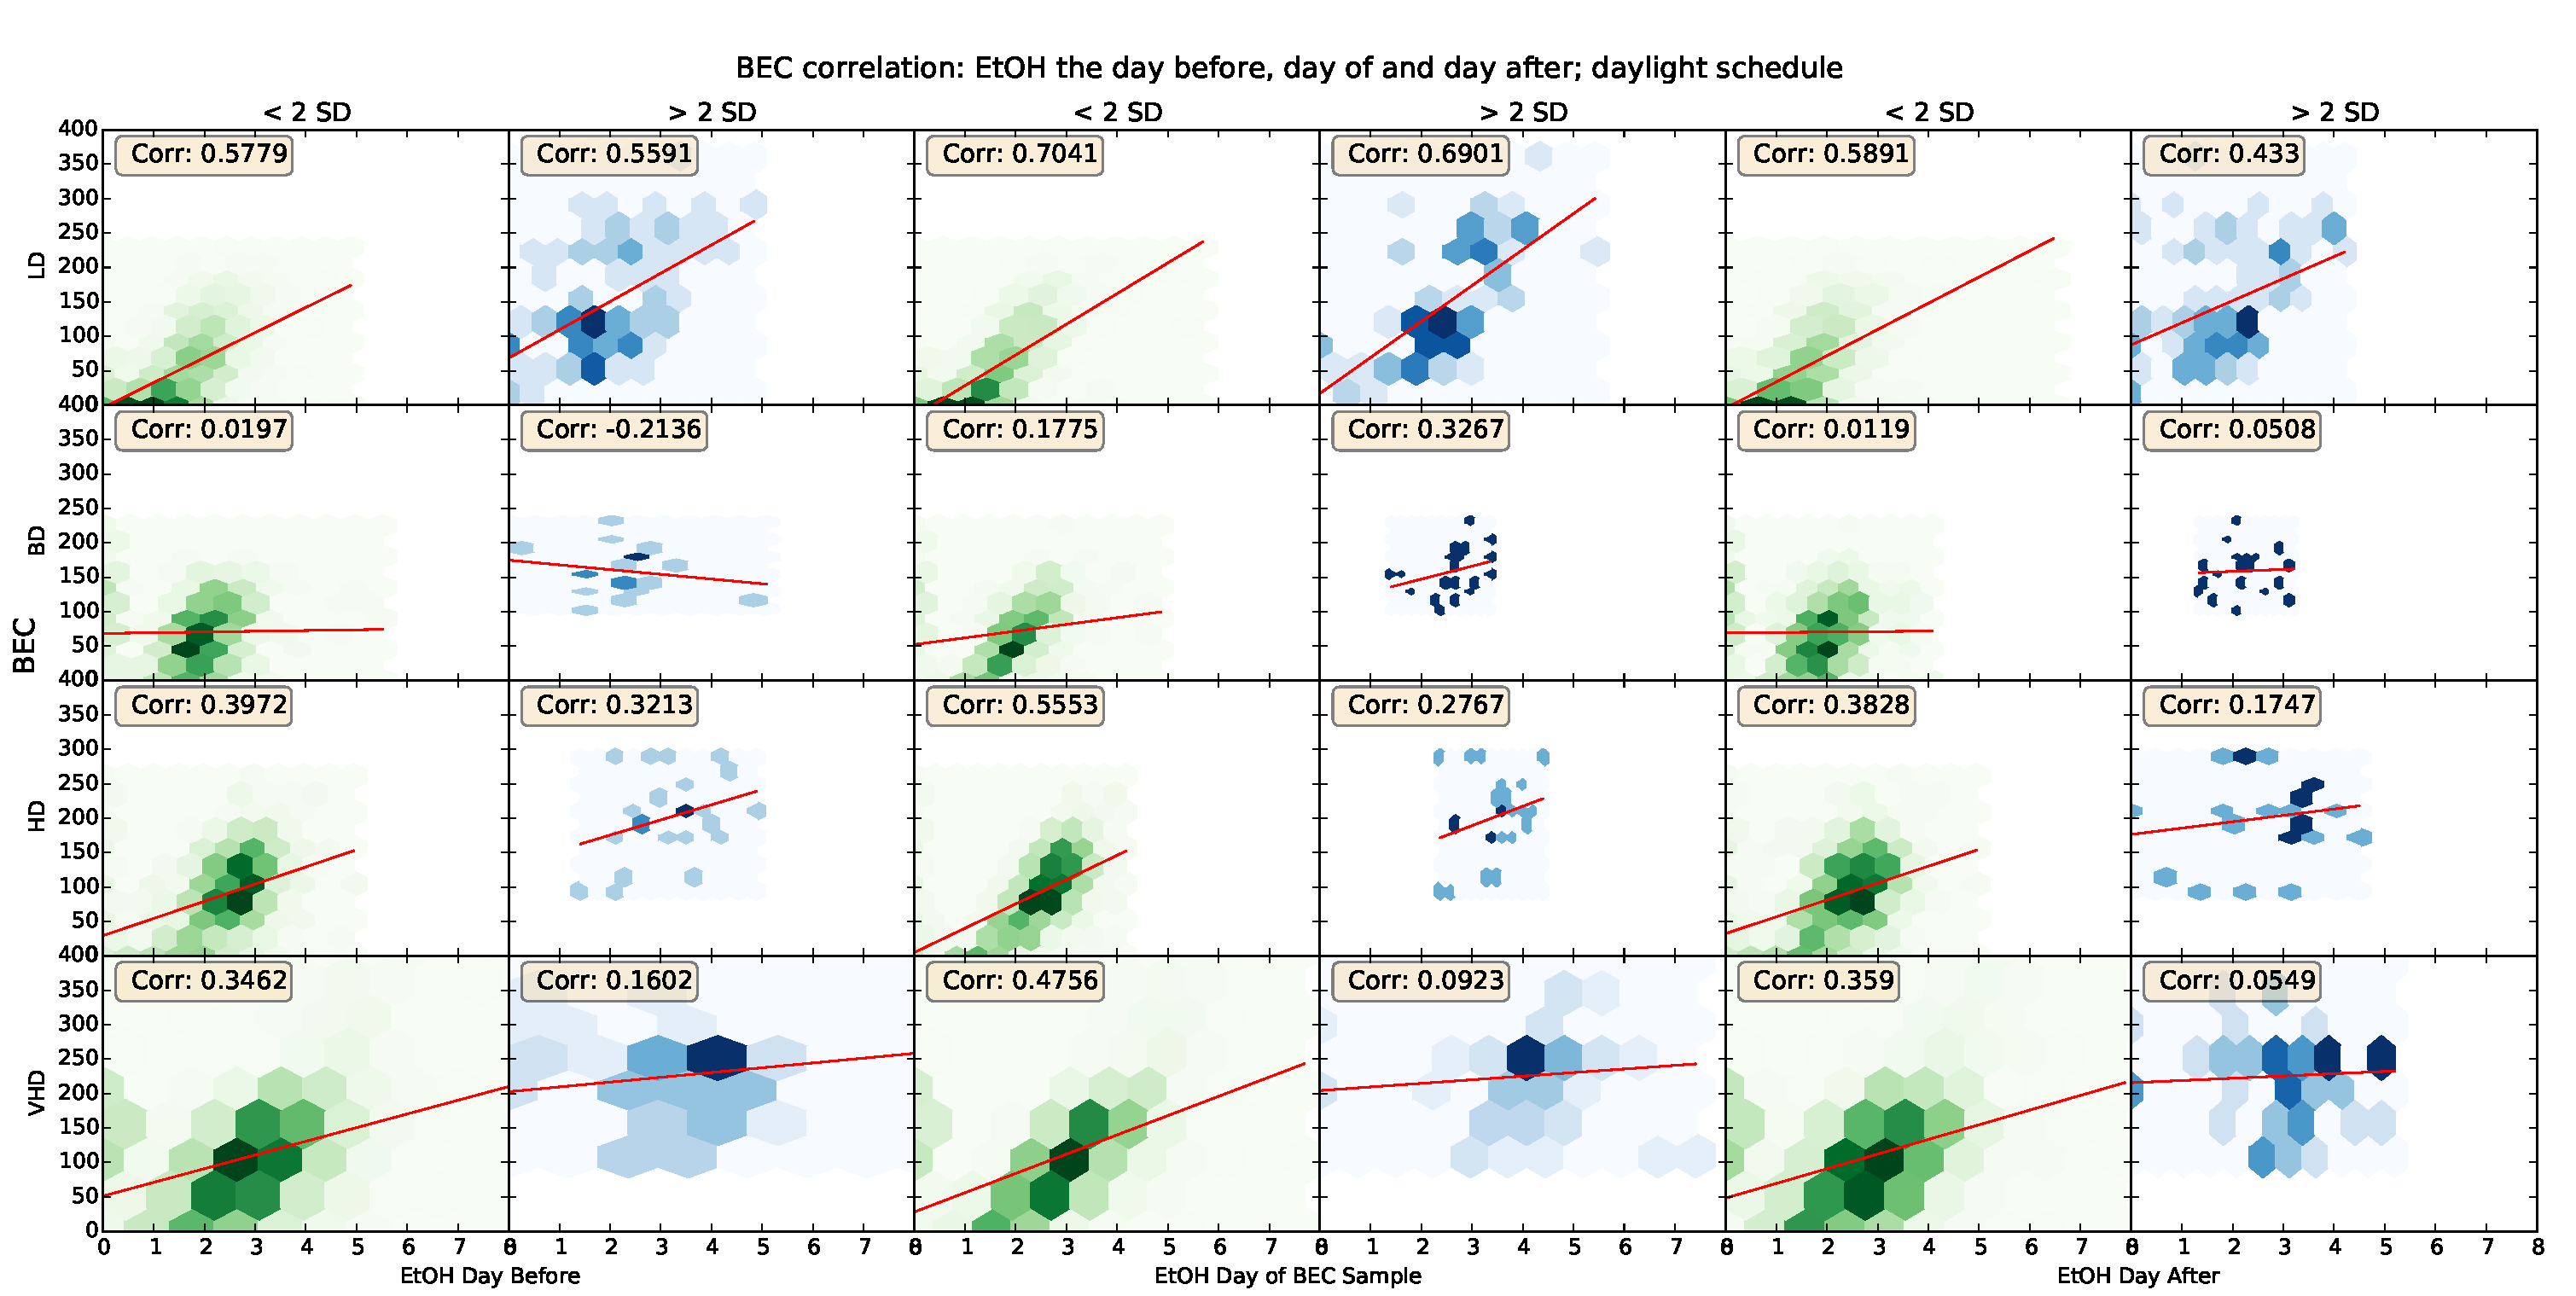
\includegraphics[width=1.2\textwidth]{figures/bec_etoh_more2std_daylight.pdf}}
		\caption{BEC $\sim$ EtOH correlation hexbin plots containing 24 panels for each DC the day before, day of and the day after BEC sample, split by intoxication event; Person correlation and linear regression fit lines are overlaid on each panel.}
		\label{fig:bec-more80}
	\end{figure}
	
	The hexbin plot could be thought of as 2D histogram and allows us to reduce the density of the data. Since it is hard to overlay the hexbin plots we now provide 24 separate panels rather than 12 combined panels. Additionally, in Figure~\ref{fig:bec-over80} we used data sorted by the \textit{daylight schedule}, which adds two hours of the last day's session. It is conjectured that animals start activities when the lab employees come to work, which happens before the lights are turned on. 
	
	First consider the correlation between the BEC level and EtOH at the sample time. On typical drinking days (no intoxication), low drinking animals (LDs) show the highest correlation, which may indicate that \textit{they do not drink much after the BEC sample}, while BDs show the least correlation, which may indicate the \textit{sporadic nature} of their drinking. On intoxication days, correlation values are less for all drinking categories, and almost not visible for VHDs, which may indicate that animals either drink much before sample (getting sober by the BEC sample time) or drink much after the sample (since VHDs have problems with stopping) - in either case BEC measurement \textit{fails to capture the true state of alcohol consumption}.
	
	Now consider Binge Drinkers (BDs). As expected, on typical drinking days with no intoxication, there is essentially \textit{no correlation} between the EtOH the day before, the day after and the BEC the day of sample is. However, on intoxication days, the amount of the ethanol consumed the day before is \textit{negatively correlated} with the BEC level the day of sample, which may indicate the effect of disliking alcohol side effects: \textit{BD animals that drunk a bit too much yesterday do not want to get intoxicated today}. 
	
	\subsection{Drinking The Day After Intoxication}
	As an extension of the BEC $\sim$ EtOH correlation study we decided to analyze the drinking the day after intoxication for all the data points available in the same males (cohorts ``5", ``7a" and ``7b") and females (cohorts ``6a" and ``6b") populations. Rather than BEC we now rely on abnormally high (for individual animal) total ethanol consumption as a measurement of the intoxication. 
	
	The first step is to find the intoxication days. Out of all drinking days (roughly eleven thousand total), days of intoxication were found as days with consumption over $\gamma$ standard deviations, for each individual animal. After trying various values for the parameter $\gamma$, it is found that the most illustrious values are in the range between 1.5 and 2. These values of $\gamma$ rendered approximately two to six percent of the days to be the intoxication days, on average.
	
	\begin{figure}[ht]
		\centering
		\makebox[\textwidth][c]{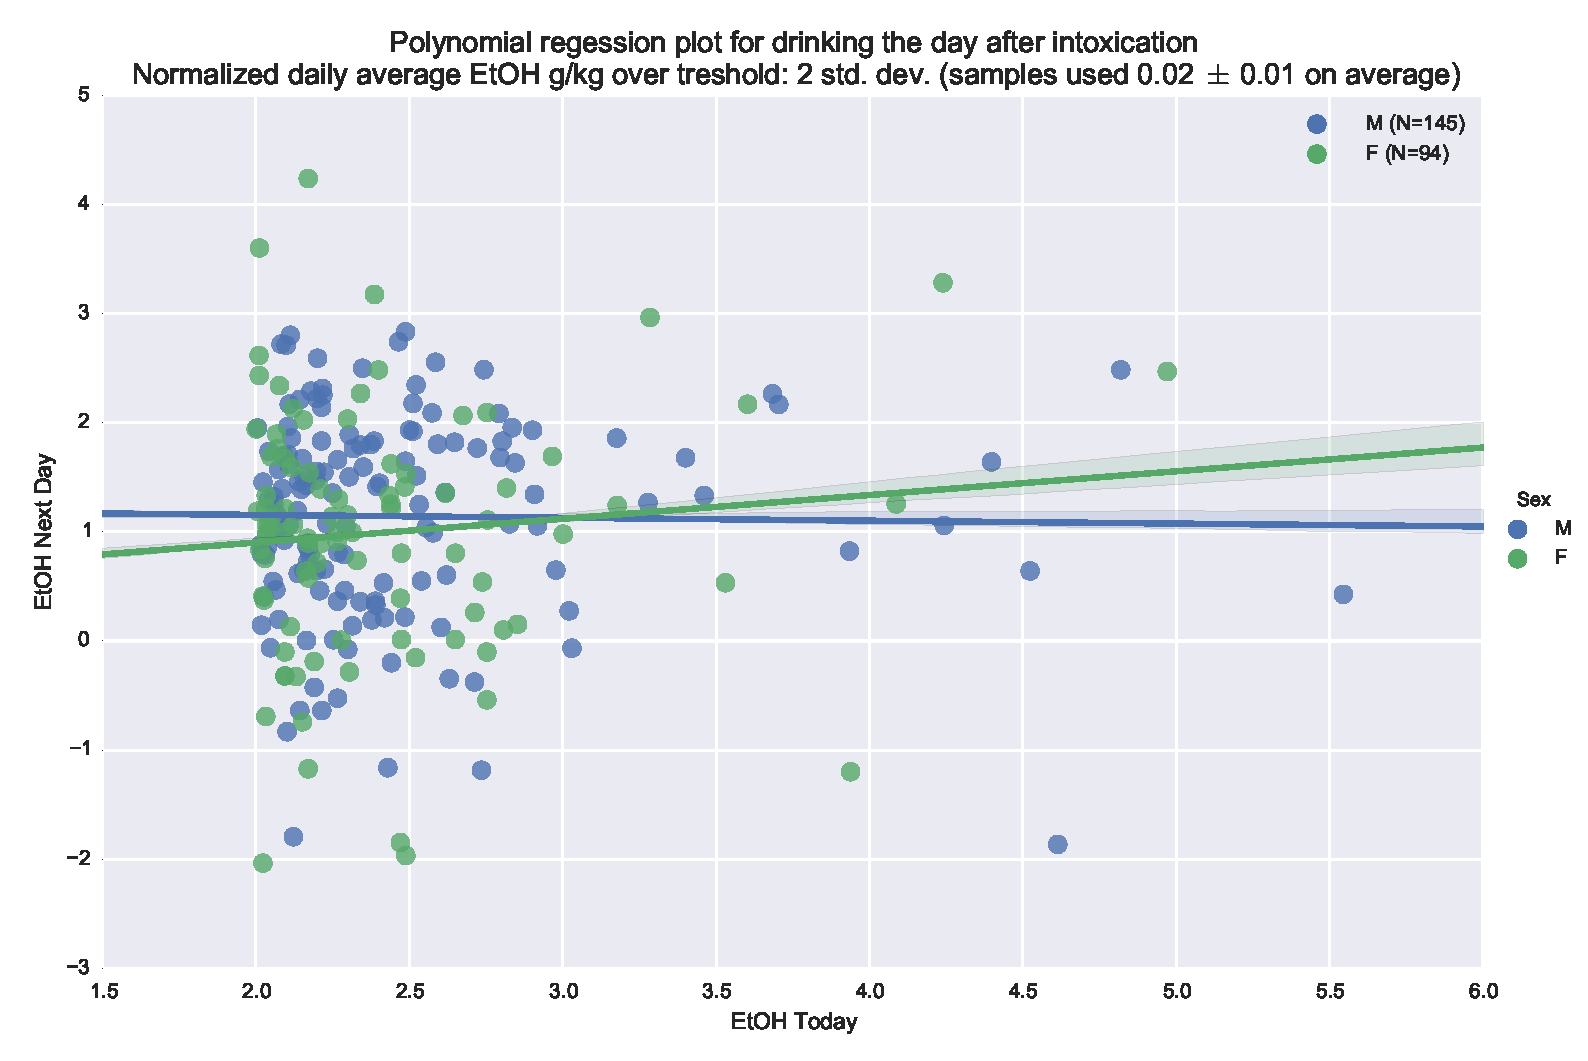
\includegraphics[width=1.1\linewidth]{figures/intox_poly-reg-factor_mf_lines.pdf}}		
		\caption{Regression plot for drinking the day after intoxication. X-axis shows the ethanol consumption (in g/kg) the day of the intoxication; Y-axis shows consumption the day after. With gender as a factor, two lines are fitted into data points.}
		\label{fig:intox-poly-reg}
	\end{figure}
		
	The second step is to collect the daily total ethanol consumption in grams per kilogram of body weight (g/kg) during days that followed the days of intoxication. The factor scatterplot of such data, along with the regression fit lines are shown on Figure~\ref{fig:intox-poly-reg}. 
	
	As expected, animals of both gender greatly reduce, on average, ethanol consumption the day after intoxication. However, as illustrated by the fitted lines, females tend to have slightly more days of heavy drinking the day after intoxication, than males. This might be due to either an internal feature of the females or a third unaccounted for factor.    
	
	Another way of looking at this data is to analyze the role of the each drinking category\footnote{"BD" drinking category is not present in the female population and was not used for this part of the study.} while compressing the change (reduction) in the drinking the day after intoxication into single average point, keeping gender as a factor. The factor line plot of that is shown on Figure~\ref{fig:intox-factor-line}. 
	\begin{figure}[ht]
		\centering
		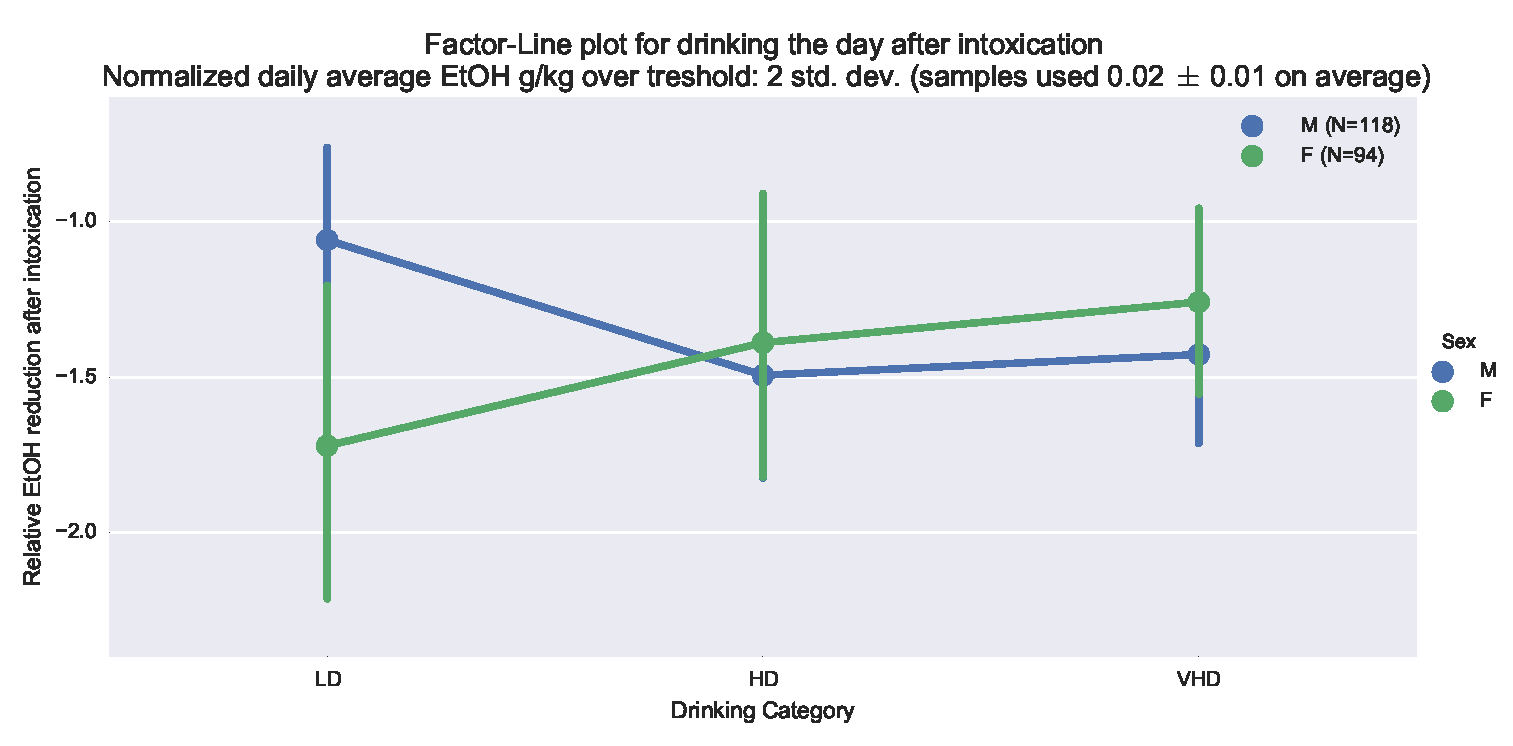
\includegraphics[width=\linewidth]{figures/intox_factor-line_mf.pdf}
		\caption{Factor-line plot for drinking the day after intoxication.  Y-axis shows the change (reduction) in drinking the day after intoxication (6\% of total drinking days), for each drinking category of X-axis.}
		\label{fig:intox-factor-line}
	\end{figure}
	
	We can see that trends are the opposite between drinking categories for two genders: very heavy drinking females tend to reduce the drinking much less the day after intoxication than low drinking ones; conversely, heavy drinking males reduce the drinking more the day after intoxication than low drinking ones.	
	
	Finally, to expand our understanding of these drinking category and gender differences in drinking after intoxication we employed violin plots. Figure~\ref{fig:intox-violin} demonstrates the distribution of the intake reduction in males and in females for each drinking category. In our case this plot does not reveal any additional information and only confirms the observations made based on the line factor plot.  	
	\begin{figure}[ht]
		\centering
		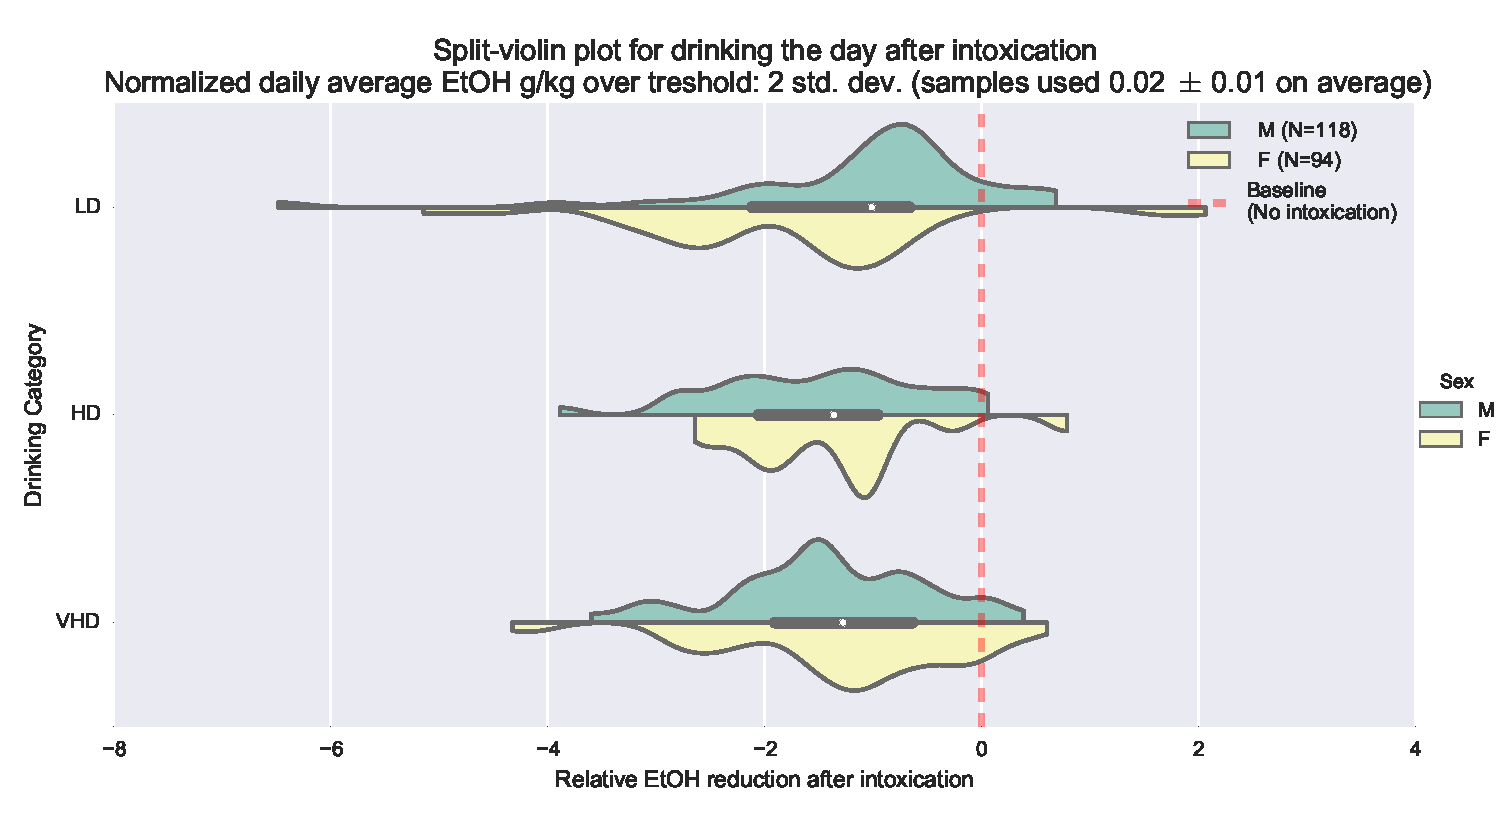
\includegraphics[width=\linewidth]{figures/intox_split-violin_mf.pdf}
		\caption{Split-violin plot for drinking the day after intoxication. Violin shows the details of reduction of drinking the day after intoxication (2\% of total drinking days), for each drinking category and for each gender.}
		\label{fig:intox-violin}	
	\end{figure}
	
	 
	
%	\begin{lstlisting}[language=Java]	
%	TM:
%	TM.releaseResources(TRID)	
%	\end{lstlisting}
\pagebreak	
\section{Predicting Future Drinkers \label{section:predicting-drinkers}}
	The following study demonstrates that data derived from the induction phase of the ethanol self-administration experiment has significant predictive power of whether or not an animal will go on to consume excessive alcohol in the future (during Open Access phase). Furthermore, we distinguish several factors tightly coupled with the probability of eventually being categorized as an heavy drinker. Early identification of risk factors in the NHP model lead to potential indicators in humans, resulting	in intervention and prevention.
	
	\subsection{Attributes' Predictive Power}
	\begin{figure}[ht]
		\centering
		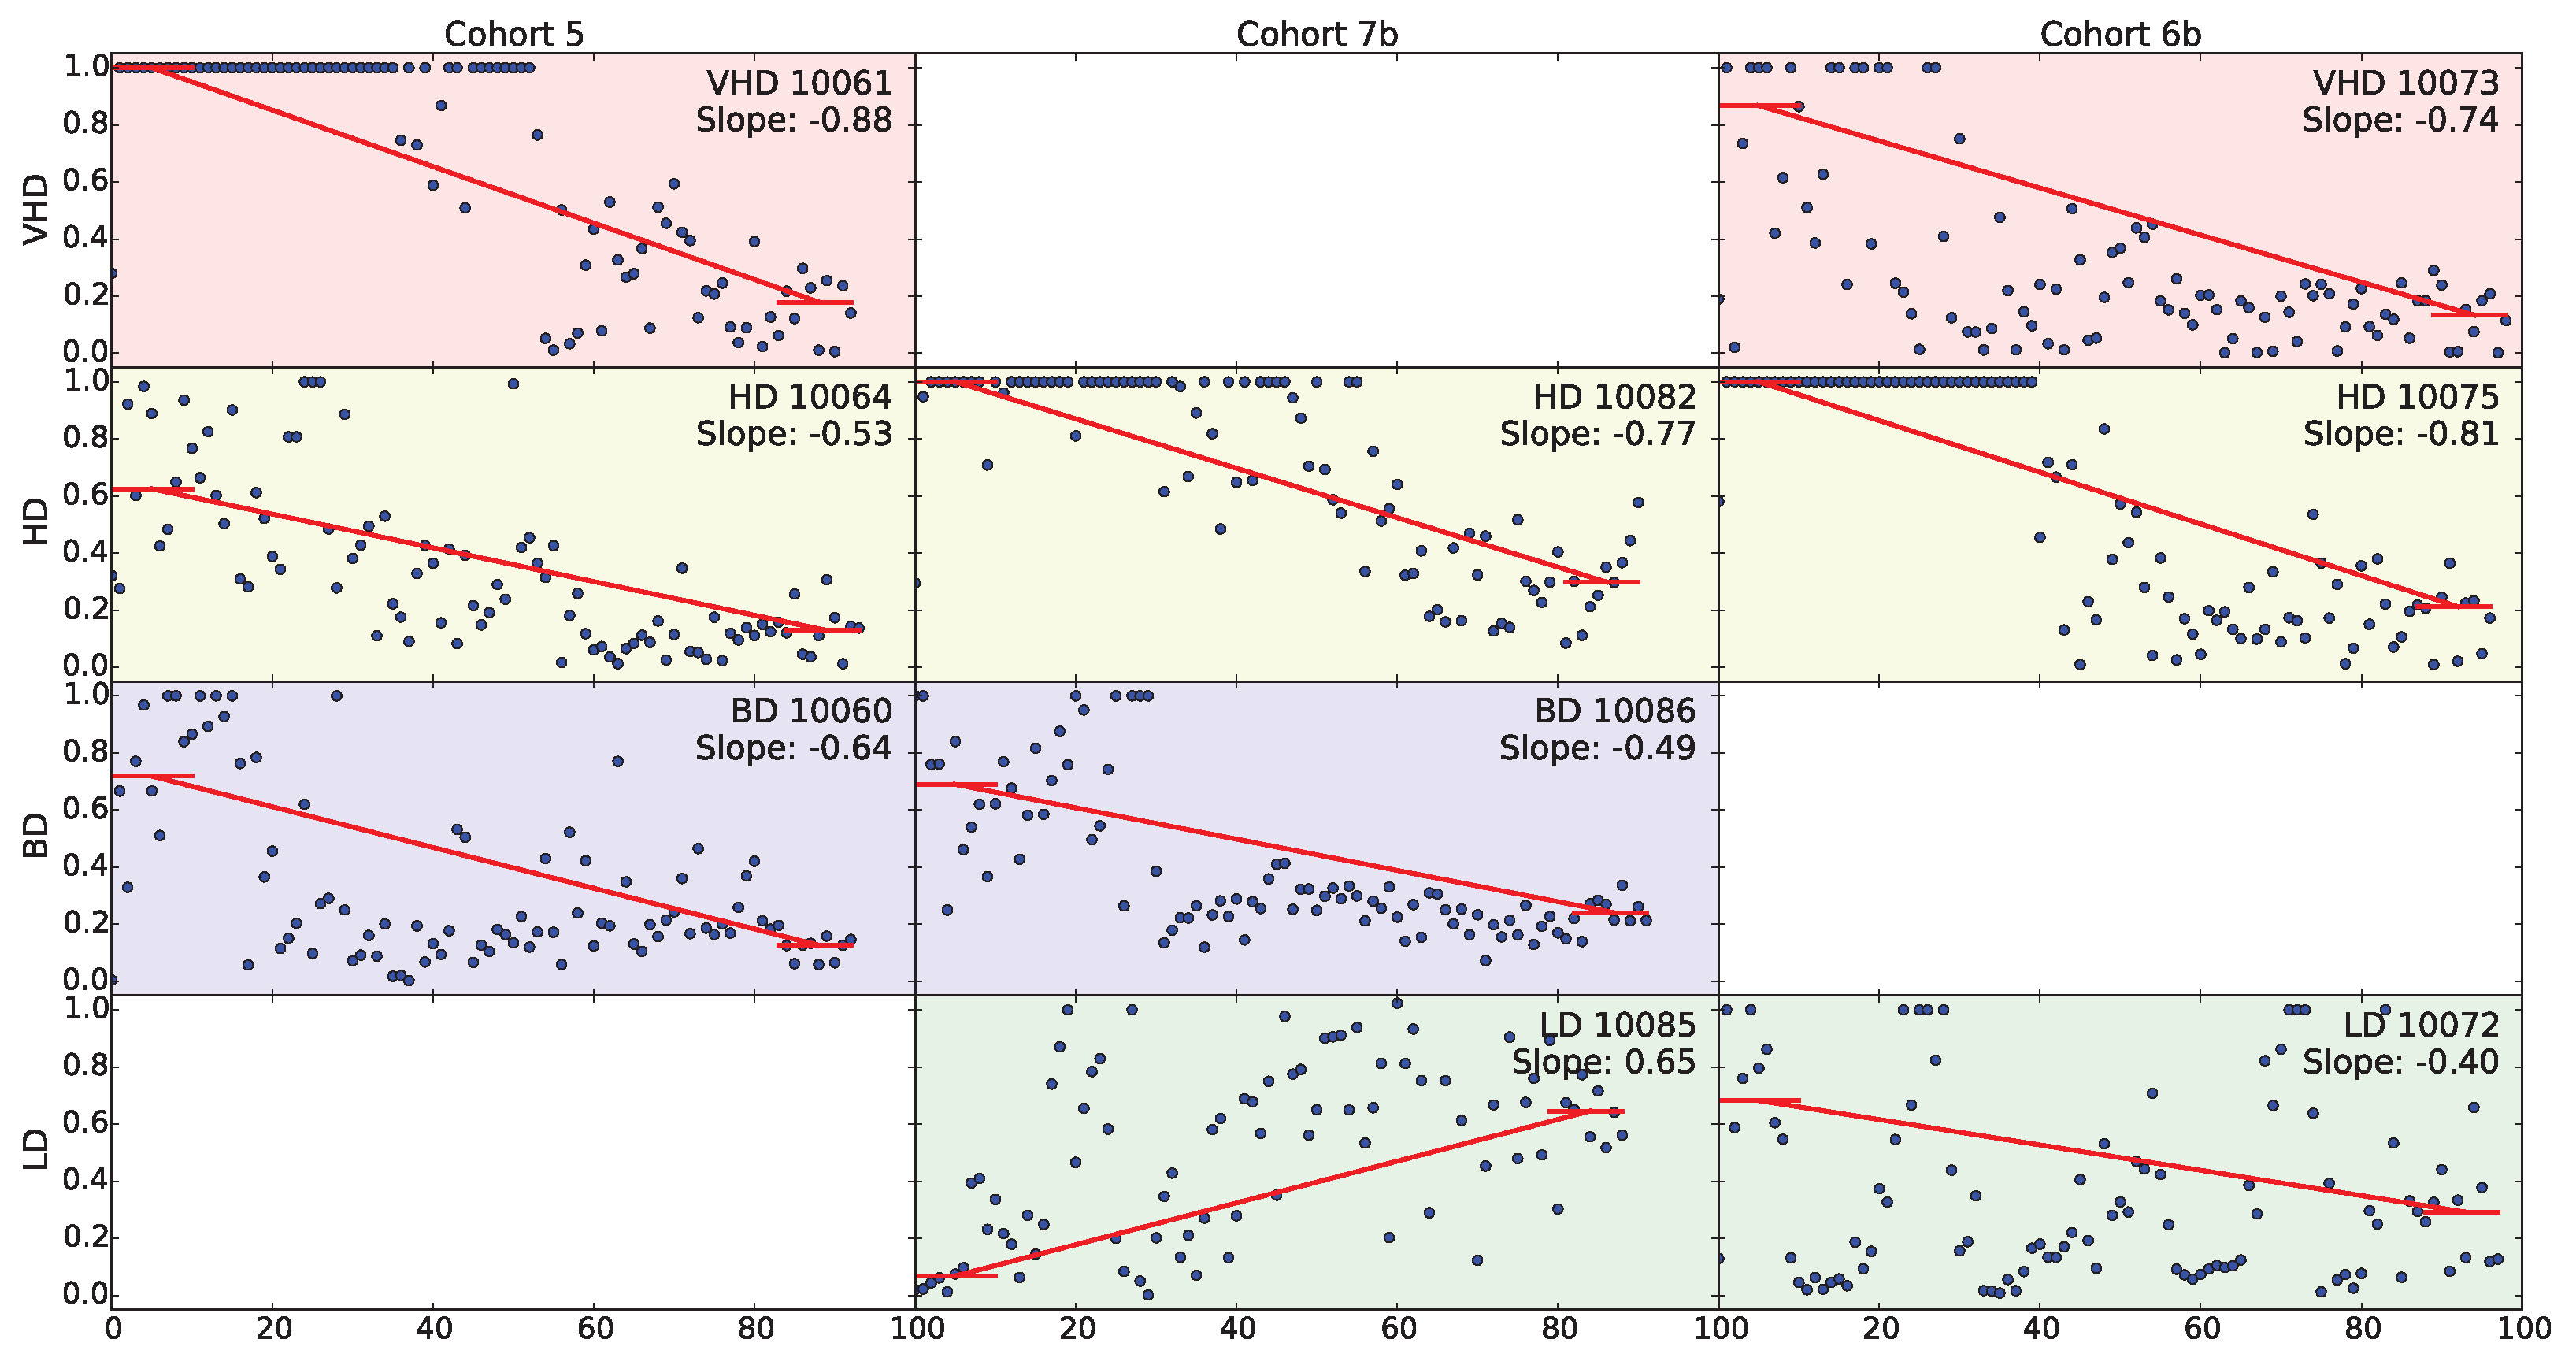
\includegraphics[width=\linewidth]{figures/attributes-predictive-power.pdf}
		\caption{Linear regression fit lines panels for each drinking category in three different cohorts illustrate persistent pattern indicating the predictive power of the attribute ``EtOH consumed during the first 10 minutes of the day, as a \% of day's total''.}
		\label{fig:attributes}	
	\end{figure}
	To demonstrate the predictive power of the attributes, consider Figure~\ref{fig:attributes}, which depicts the EtOH consumed during the first 10 minutes of the day, shown as a percent of the daily allotment. The plots are broken down by drinking categories and cohorts. From the figure we notice that the slope tends to be step negative for VHD and flattened step or even positive for LD. This difference indicates that the EtOH consumed during the first 10 minutes of the day is a potential prediction feature. 


	\subsection{Feature Generation}	
	Having over 20 raw and derived attributes we generated over 60 features in form of relative deltas as described in \cref{section:feature-generation}.
	\begin{figure}[ht]
		\centering
		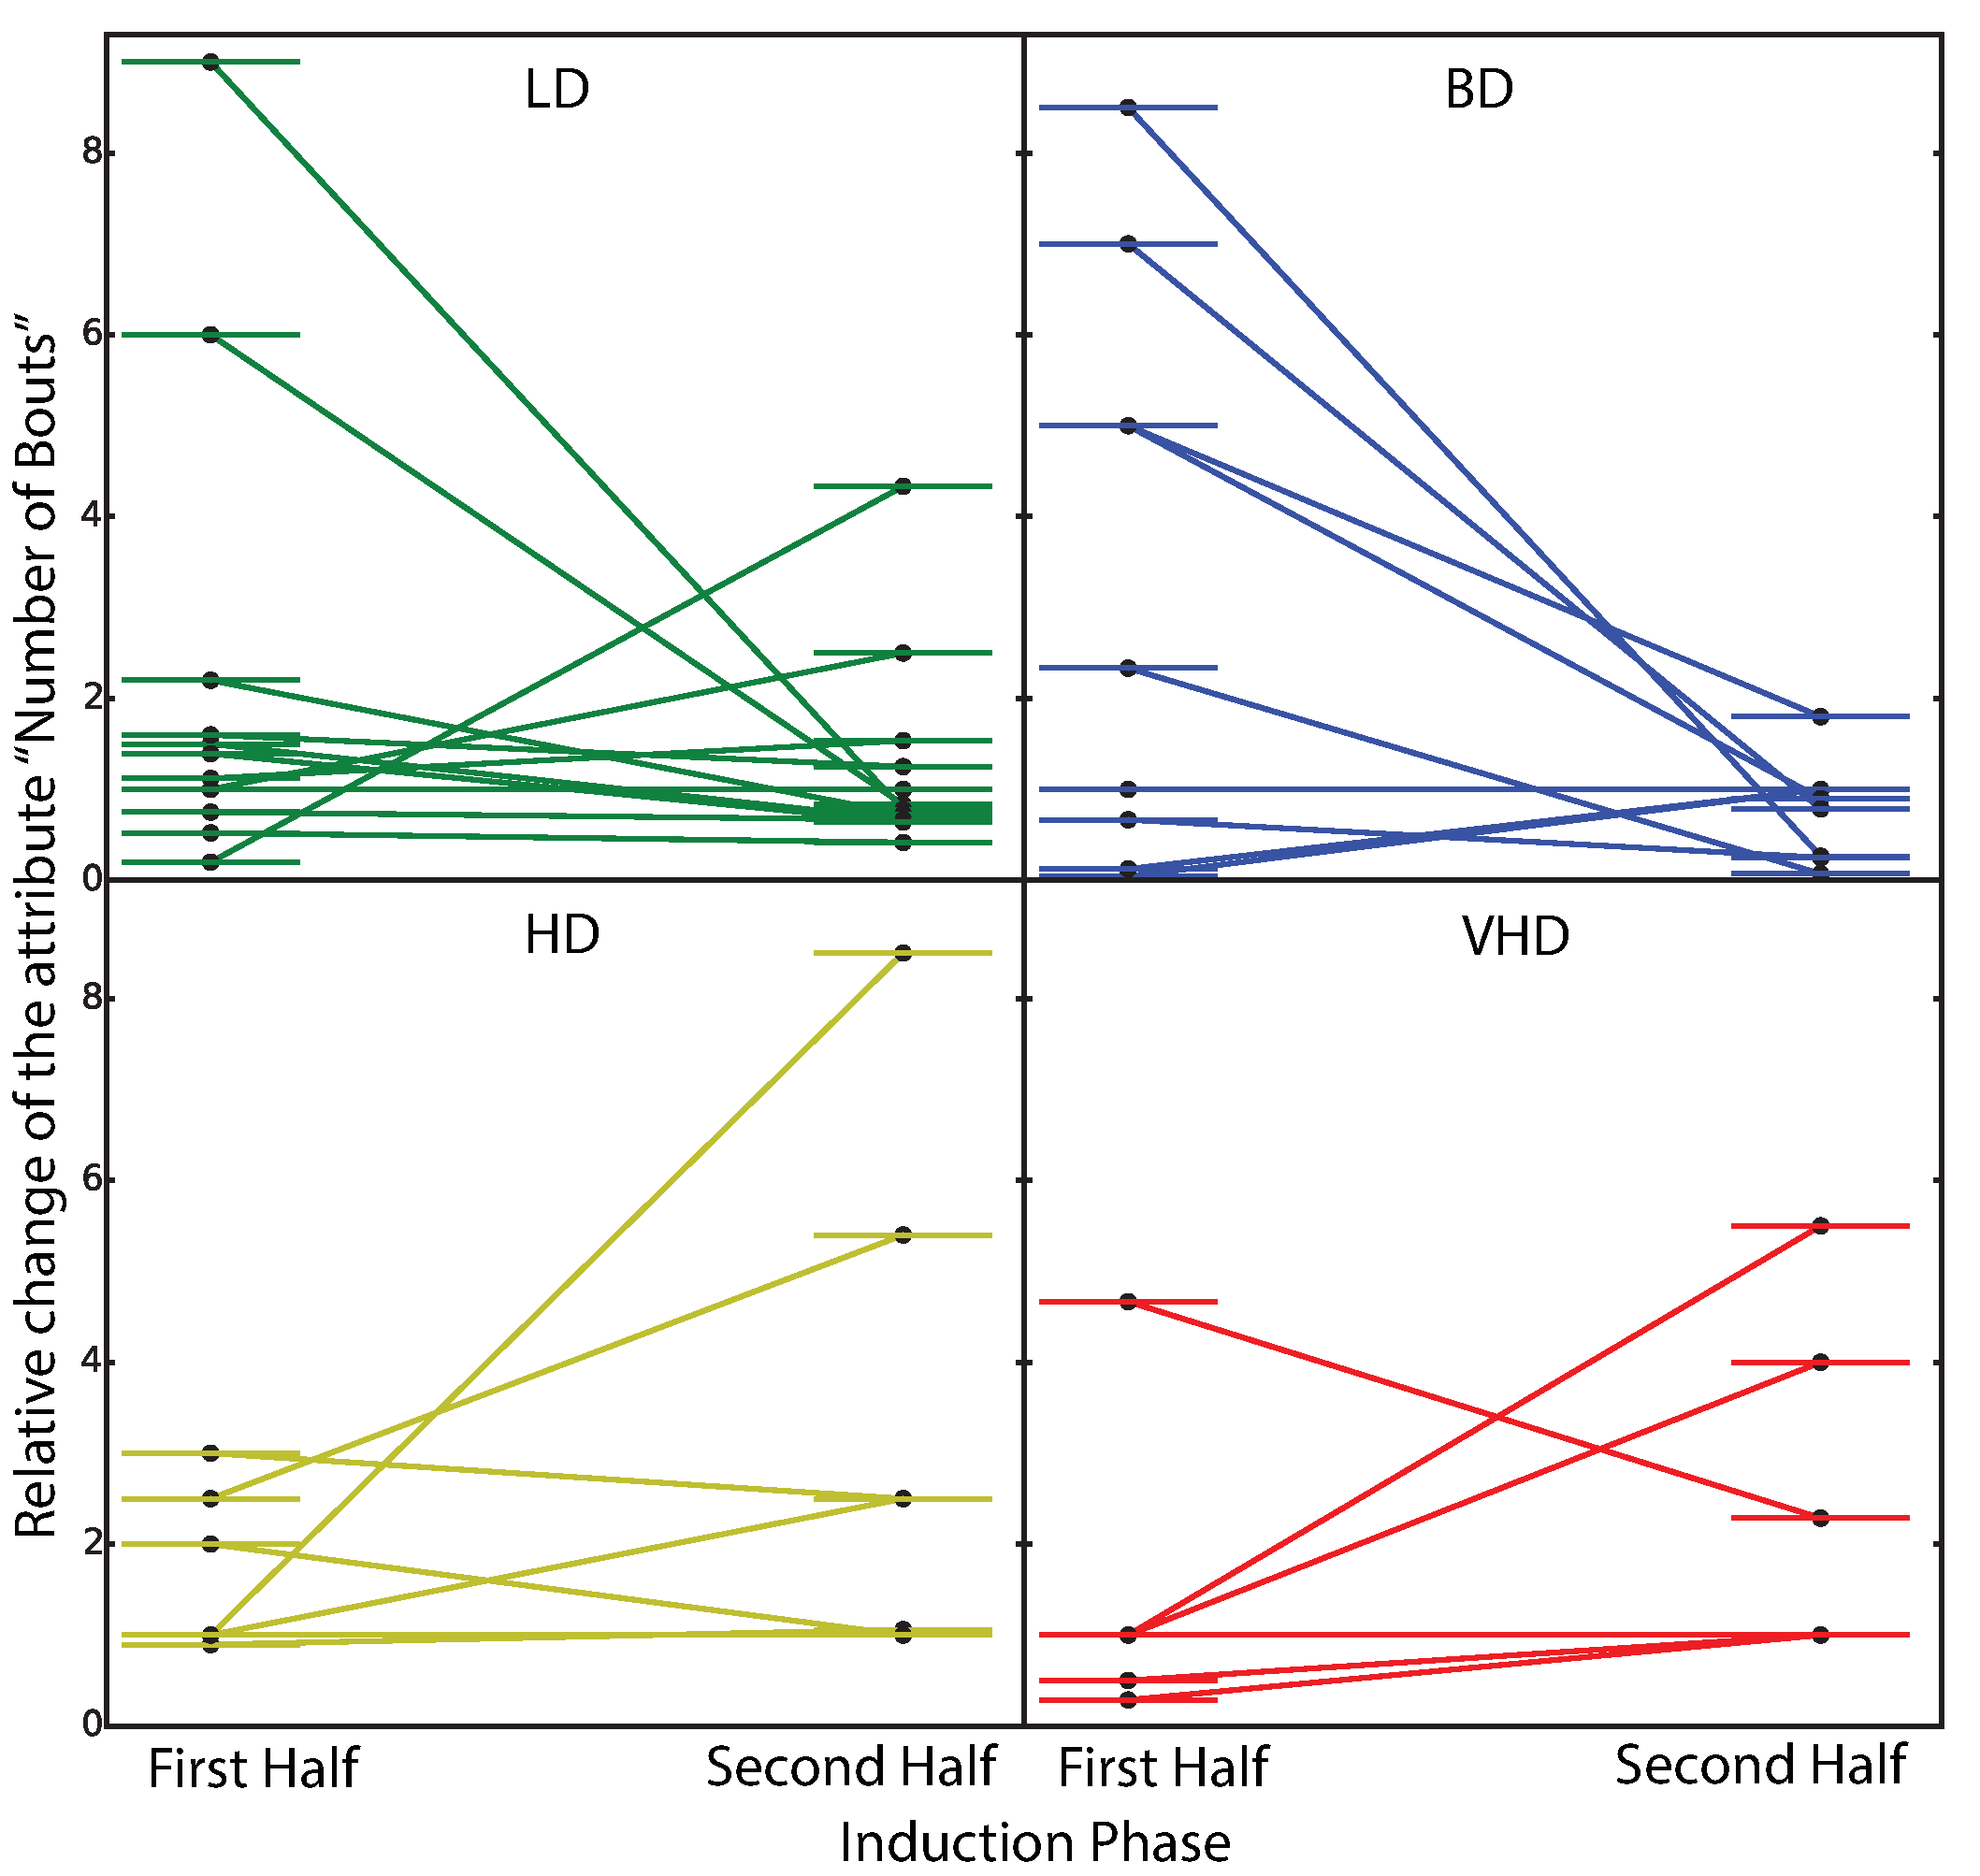
\includegraphics[width=0.8\linewidth]{figures/rel_change_num_bouts.pdf}
		\caption{Intra-cohort relative deltas panels for each drinking category illustrates persistent pattern in feature ''total number of EtOH bouts".}
		\label{fig:rel-change-bouts}	
	\end{figure}
	
	To illustrate the utility of relative deltas, Figure~\ref{fig:rel-change-bouts} displays the panel with relative deltas for the total number of EtOH bouts by a monkey during a 22-hour drinking session, divided into four subplots by drinking category. On the left of each plot, the figure indicates the relative change between the median values of phase one to phase two; on the right of each plot, the figure shows the relative change from phase two to phase three. The vertical axis represents the results from dividing the later median by the former. Low drinking animals, shown in the top row of the figure, generally decreased the total number of EtOH bouts on the later stage of the induction period (which could indicate either more aggressive bouts or less overall ethanol consumption), while high drinking animals generally increased by that same number. In this case, the calculation of relative deltas represents good predictors, or good features, because they describe the temporal process of drinking behavior adaptation. This is in-line with previous findings indicating that the third phase of induction, which is used to calculate relative deltas, is one of the most significant attributes in predicting drinking behavior \shortcite{grant2008drinking}.
	
	\subsection{Feature Filtering}
	Many features with small sample size lead to mathematically undetermined solutions. To filter the feature space we eliminated statistically non-significant features by performing significance tests ($\alpha=0.1$) and mutual information analysis. That leaves us with the most significant features shown in Figure~\ref{tab:feat-most-signif}, grouped by categories and ordered by p-value (decreasing top to the bottom). 
	
	A feature filtering step is used for selecting the best model. Later in this study we select a basis model and build on top of it. That novel model is developed using a feature selection technique, as described in \cref{section:feature-selection}.
	
	\begin{table}[h]
		\centering
		\caption{Feature space filtered by statistical significance.}
		\label{tab:feat-most-signif}
		\begin{tabular}{lll}
			\hline
			\abovespace\belowspace
			Feature & Phase & p-value\\
			\hline
			\multicolumn{3}{c}{Natural}\\
			\hline
			Age of intoxication & natur. & .004\\
			Age & natur. & .005\\
			Sex & natur. & .065\\
			\hline
			\multicolumn{3}{c}{Drinks}\\
			\hline
			Mean length for EtOH drinks & $\Delta_2$ & .003\\
			Mean volume for EtOH drinks & $\Delta_{total}$ & .014\\
			Median time between EtOH drinks & $\Delta_{2}$ & .036\\
			\hline
			\multicolumn{3}{c}{Bouts}\\
			\hline
			Total number EtOH bouts & $\Delta_{2}$ & .030\\
			Max bout volume as \% of total EtOH & $\Delta_{2}$ & .047\\
			Time to reach day's allotment & $\Delta_{2}$ & .097\\	
			\% EtOH during first 10 minutes & $\Delta_{1}$ & .080\\	
			Latency to first drink & $\Delta_{2}$ & .093\\
			Max bout length & $\Delta_{1}$ & .100\\			
			\hline
		\end{tabular}
	\end{table}

	\subsection{Model Selection}
	To select the basis model for the classification task we tested several models, see \cref{section:ml-models}. Acknowledging the noisy data with small sample size we tested each model with and without an applied bagging wrapper. Our hypothesis, regarding bootstrap aggregation, was that it should significantly improve the accuracy of Random Forests as suggested by \shortcite{breiman1996bagging}, but leave the Gradient Boosting without considerable changes since it natively incorporates its own special sampling technique. Ultimately, we could not draw hypothesis with regard to SVM. 
	
	\subsubsection{Support Vector Machines}
	We trained SVM models with various combination of parameters, as shown provided in Table~\ref{tab:svm-pars}. 
	
	\begin{table}[h]
		\centering
		\caption{Tested domain of settings for SVM classifier.}
		\label{tab:svm-pars}
		\begin{tabular}{lll}
			\hline
			\abovespace\belowspace
			Kernel	& Penalization Factor & Class Weights\\
			\hline
			Linear	& C = 1 & Yes\\
			Rbf (exponential) & C = 2 & No\\
			Polynomial & C = 3 &\\
			Sigmoid & C = 4 &\\		
			\hline
		\end{tabular}
	\end{table}
	
	Kernel could be thought as a similarity measure. Penalization factor sets the cost for the data that does not fit the current model; increasing C yields a more complex model (more feature are selected). Using class weights allow to counteract the problem of classes with unequal size. After repetitive experiments, model with the linear kernel and penalization factor C = 3 using sample weights proved to be the best option, having the mean accuracy, on average over multiple runs, equal 0.51 (SEM=.08). 
	
	\subsubsection{Random Forests}
	Random Forests (RF) are known to be very robust to the noise and to give good results while working fast.
	After repetitive experiments, we found the model with the following parameters to give the best accuracy: number of estimators=10, criterion=``gini", no max depth restriction, min samples split=2, min samples leaf=1, max features=0.4, bootstrap=True. This model yields a mean accuracy of .50 (SEM=.11), on average, which is not worse than SVM yet has greater variance. 
	
	\subsubsection{Gradient Boosting Classifier}
	A gradient Boosting (GB) classifier is an additive model in a forward stage-wise fashion; it allows for the optimization of arbitrary differentiable loss functions. In each stage, n-classes regression trees are fit on the negative gradient of the binomial or multinomial deviance loss function. Furthermore, it allows for sampling with the replacement with varying percentage of usage for number of features and number of examples used while training each individual tree. The best parameters for the model are: number of estimators = 200, max samples = 80$\%$, max features = sqrt, bootstrap = true. Thus, each of the 200 regressors trees had sampled, with replacement, set with size equals 80 $\%$ of examples, and, most importantly, with number of features equal square root of total number of available features. With that, GB yielded the mean accuracy of 56$\%$ (SEM=.1), on average. That is significantly better than both Random Forests and SVM yet variance kept in bounds. 
	
	\subsubsection{Bagging Wrapper}
	Since we have only 50 samples, and getting more is both costly and unethical, we tried to artificially sample (with replacements) more examples. Given arbitrary abundant feature sets we leave some of them behind in order to compensate for potentially meaningless features. That is exactly what Bagging Wrapper is meant to do with previous classifiers. Table~\ref{tab:ml-model-results} describes how bagging influences the classifiers and provides overall accuracy measures for each tested classifier along with the naive classifier described in \cref{section:performance-measure}. 
	
	\begin{table}[h]
		\centering
		\caption{Experimental accuracy results for different classifiers.}
		\label{tab:ml-model-results}
		\begin{tabular}{lll}
			\hline
			\abovespace\belowspace
			Classifier	& No Wrapper	& Bagging Wrapper \\
			\hline
			Naive & \multicolumn{2}{c}{0.32}\\
			SVM	 	& 0.51 (SEM=.08)	&	0.42 (SEM=.09)\\
			RF	&	0.50 (SEM=.11)	&  \textbf{0.61 (SEM=.07)}\\
			GB & 0.56 (SEM=.10)	& 0.57 (SEM=.10) \\	
			\hline
		\end{tabular}
	\end{table}
	
	Cohesive with our initial hypothesis, while Random Forests drastically improved its accuracy, Gradient Boosting result exhibit minimal change since it already incorporated some of the bagging technique and too extreme samples of bagging might have hurt the features gradients.
	
	SVM actually decreased its accuracy when used in conjunction with bagging. This might be explained by the fact that the regularization parameters for this model were fine tuned on the given dataset of 50 examples, thus sampling more of them destroyed the accurate settings of the model.
	
	To understand the difference in trade-off between the random forests and gradient boosting we could think of the fact that the better generalization property of ensemble approach is often explained using the classic bias-variance decomposition analysis. Specifically, previous studies pointed out that methods like bagging improve generalization by decreasing variance while methods similar to boosting achieve this by decreasing
	bias\footnote{In the article cited reader can find a visual representation of the mentioned differences.} \shortcite{yang2010review}.
		
	Given the above results, a random forests model with a bagging wrapper was chosen as basis model to perform two-step classification.	
	
	\subsection{Novelty Two-Step Classification Model}	
	The problem in our classification task is that given small sample size (50 animals) and uneven drinking class size distribution it is hard to train a good classifier. Thus we decided to perform classification in the two-steps. We first aggregated the four categories into two: ``LD and BD" and ``HD and VHD", essentially producing ``Heavy vs. Non-Heavy Drinkers". Then we used the basis RF model with bagging, but this time deploying forward selection strategy to rank the importance of each feature in order to reduce feature set dimensionality. Detailed description for feature selection procedure is provided in \cref{section:feature-selection}, but  essentially the process ranks the features by their impact on model performance. This process was a major computational bottleneck in building the classification model and took approximately 15 minutes each time. 
	
	During the first step, the classification accuracy for two groups reaches 82\%, and the best when using four features, as shown on the Figure~\ref{fig:forward-selection-combined}. There are three options on how to pick the features then. Initially, during each run of the feature selection procedure, we assigned the rankings to each feature, then we picked the top-4 most popular features according to the cumulative ranking. Another attempt was to rank features by the number of appearances in the top-4 list, simulating the essentialness of the features. Unexpectedly, both methods proved to be inferior to merely \textit{picking the top-4 features out of the best run}. That may be due to the fact, that feature selection process appends features \textit{based on their collaborative performance}, thus \textit{most popular features do not necessarily work well together}. 
	
	\begin{figure}[ht]
		\centering
		\includegraphics[width=\linewidth]{figures/feature-selection-heavy-non-eps-converted-to.pdf}
		\caption{Feature selection process for heavy vs. non-heavy drinkers.  The horizontal axis represents the number of features chosen based on contribution. The vertical axis shows the average accuracy of the drinking category classification. Base accuracy shows naive guess.}
		\label{fig:forward-selection-combined}
	\end{figure}
	
	On the second step, aggregated categories were subsequently reclassified into their individual inherent categories: non-heavy drinkers into LD and BD, heavy drinkers into HD and VHD. The feature selection procedure produced the set of features that results in the best average accuracy. Table~\ref{tab:selected-features} provides a summary of selected features during each step and the average accuracy.
	
	\begin{table}[htb]
	\centering
	\caption{Set of features chosen by \textit{Forward Selection} algorithm for two-step model classification. For each of the three classification tasks the sets of selected features are different which may relate to the different nature of behavioral characteristics between difference drinking groups.}
	\label{tab:selected-features}
	\begin{tabular}{ll}
	\hline
	\abovespace\belowspace
	\toprule Feature & Phase  \\ \midrule		
	\multicolumn{2}{c}{\textit{Heavy vs Non-Heavy Drinkers (accuracy=0.82)}} \\
	Number of EtOH bouts & $\Delta_2$ \\
	Mean length for EtOH drinks &  $\Delta_1$\\
	Mean volume for EtOH drinks & $\Delta_1$\\
	Age & \textit{fixed}\\ 
	
	\midrule
	\multicolumn{2}{c}{\textit{Low vs Binge Drinkers (accuracy=0.91)}} \\
	Mean length for EtOH drinks &  $\Delta_2$\\
	Latency to the first drink & $\Delta_{total}$\\
	
	\midrule
	\multicolumn{2}{c}{\textit{Heavy vs Very Heavy Drinkers (accuracy=0.89)}} \\
	\% of days EtOH consumed in first bout &  $\Delta_{total}$\\
	EtOH during first 10 minutes of the day & $\Delta_{total}$ \\ 	
	\bottomrule
	\end{tabular}
	\end{table}
	
	For the heavy vs. non-heavy drinkers classification we can achieve a 82\% accuracy rate with four features: total number of EtOH bouts, mean length and volume of EtOH drinks, and age. Distinguishing between subgroups appears to be even more accurate, however that is due to  fact that the class size distribution is more skewed within the subgroups. 
	
	Observing the absence of common features between classification of two sub-groups indicates that the differentiation between HD and VHD is markedly distinct from the differentiation between LD and BD. This may relate to the different nature of behavioral characteristics between difference drinking groups. Notably, for HD and VHD, both features are associated with the drinking within the first minutes of the day, while for distinguishing heavy and non-heavy drinkers the mean values describing drinks are predicative.


	\subsection{Model Validation}
	To validate the model we calculated two-step composite average accuracy and the by-cohort accuracy using the evaluation tools described in \cref{section:accuracy-evaluation} and \cref{section:performance-measure}.
	
	\subsubsection{Two-Step Composite Average Accuracy} Total, or composite, accuracy is calculated for the entire model by determining category distribution and the accuracy rates for both the first and second steps. The prior probability of a sample being in the group ``LD and BD" is 52\%, while the prior probability (or likelihood) of being in the group ``HD and VHD" is 48\%. Accordingly, the probability-adjusted accuracy of being correctly classified within the Heavy and Non-Heavy groups is 82\%. The first step accuracy of 82\% and formula~\ref{eq:composite-accuracy} is used to composite average accuracy. \textit{P} denotes the prior probability (or likelihood) in [0..1] format; \textit{A} denotes accuracy: 
	\begin{equation}
	\begin{split}
	A_{comp.} &= A_{1^{st}step}*(P(non-heavy)*A_{LD vs. BD} + P(heavy)*A_{HD vs. VHD})\\
			&= 0.82*(0.48 * 0.89 + 0.52*0.91) = 0.74
	\end{split}
	\label{eq:composite-accuracy}
	\end{equation}
	
	To measure the improvement of the composite average accuracy of 74\% we compare it to the base case accuracy. To calculate the base case for two-step classification by choosing the most likely categories during both steps. In the first step, the most likely group is ``LD and BD" with a 52\% probability of being correct. In the second step, the most likely category is LD with a 62\% probability of being correct. Thus, the overall accuracy for a two-step naive classifier is 32\%. Our classification strategy represents approximately a 2.5 fold performance improvement over a naive probabilistic way of predicting the correct result. 
	
	
	\subsubsection{Cohort Accuracy} While animals come from different cohorts, their common experimental protocol backgrounds enable an evaluation of common behavioral features that may help to predict future drinking associated with AUDs. Examination in a cohort-centric manner, however, reveals information about cohort specific behavior. 
	
	To calculate the accuracy by cohort, instead of random folds as in cross-validation we used cohorts division as natural folds. For each such fold (cohort) we trained the model on all the other examples outside of the fold and then tested on the chosen fold\footnote{Importantly, the cohort id information was unavailable for the model which otherwise would have made the task much simpler due to the skewed DC distribution within cohorts.}. Table~\ref{tab:by-cohort-heavy-non} provides the results of the first step classification accuracy by cohort. Such table were also create for two classification tasks of the second step and could be found in Appendix A, Table~\ref{tab:by-cohort_ld_bd} and \ref{tab:by-cohort_hd_vhd}.
	
	\begin{table}[h]
	%---HEAVY VS NON-HEAVY
	\centering
	\caption{First step (heavy vs non-heavy) classification accuracy using cross-validation with the cohorts as natural folds.}
	\label{tab:by-cohort-heavy-non}
	\begin{subfigure}{0.3\linewidth}  \centering	
	\begin{tabular}{ll}	
		\hline
		\abovespace\belowspace
		\toprule Cohort & Accuracy\\ \midrule
		Rhesus 4 &  0.7\\
		Rhesus 5 & 0.625\\
		Rhesus 6a &  0.83\\
		Rhesus 6b & 1.0\\
		Rhesus 7a & 0.5\\
		Rhesus 7b &  0.8\\
		Rhesus 10 & 0.875\\ \bottomrule
	\end{tabular}
	\caption{Accuracy \label{table:by-cohort-accuracy-twocases}}		
	\end{subfigure}
	\begin{subfigure}{0.3\linewidth}\centering
	\begin{tabular}{ccc}
		\toprule  & \multicolumn{2}{c}{Predicted DC}\\ 
		\cmidrule(r){2-3}
		DC & Heavy & Not \\ \midrule
		Heavy & 5 & 21 \\
		Not & 16 & 8\\ \bottomrule
	\end{tabular}
	\caption{Confusion Matrix \label{table:by-cohort-cm-twocases}}		
	\end{subfigure}	
	\begin{subfigure}{\linewidth}\centering
		\begin{tabular}{lllll}
			\toprule DC &  precision  & recall & f1-score  & support\\	\midrule
			Heavy    &   0.72   &   0.81   &   0.76    &    26 \\
			Non-heavy     &  0.76   &   0.67   &   0.71    &    24\\
			Avg / Total    &   0.74   &   0.74   &   0.74   &  50\\ \bottomrule
		\end{tabular}
		\caption{Per class recall, presicion, f-measure and support\label{table:by-cohort-cm-details-twocases}}	
	\end{subfigure}	
	\end{table}
	
	While our classifier performs relatively well, since cohort sizes are extremely small it is difficult to use intra-cohort predictions as the basis for inter-cohort hypotheses development or to draw conclusions about the population in total. 


	\subsection{Partial Dependencies}
	The downside of the RF classifier is that it is hard to infer the features influence onto target variable. In our case we are interested to see how each feature, or combination of features, affects the likelihood of the later drinking category classification to the animal. We use partial dependency plots (PDP) to facilitate the visual understanding of the dependence between the likelihood of becoming very heavy drinker (VHD) and a set of target features, marginalizing over the values of all other features. 	
	
	\begin{figure}[ht]
		\centering
		\includegraphics[width=0.8\linewidth]{figures/pdp5-eps-converted-to.pdf}
		\caption{Partial dependence plots (PDP) illustrate the dependence between the two target features (maximum bout length and mean length of EtOH drinks) and the likelihood of becoming VHD (top row) or LD (bottom row).}
		\label{fig:pdp5}
	\end{figure}
	
	Figure~\ref{fig:pdp5} provides two PDP plots. Top row describes the dependence between two target features and the likelihood of becoming VHD. Feature relative change of the tendency (mean or median) is normalized by standard deviation and adjusted by animal's weight and plotted on the x-axis. Feature values represent fold changes: a value of 2 on x-axis means that animal increased the value of this attribute two-fold during the induction, while value 0.5 means decreasing two-fold. 
%	Vertical bars on the x-axis represent a sample used for the line approximation. 
	
	First, consider the feature ``Max bout length". There is a linear relationship that implies animals that increased their maximum bouts’ length during the induction are very likely to become VHD later on. That may indicate that, in general, future VHD animals prefer alcohol and start to enjoy it and prolong their maximum bouts in time. However, there are several VHDs that do not fit that pattern, and while they increased their max bouts' length significantly they were less likely to become VHD. This constitutes either a factor unaccounted for or the erroneous classification method for that specific animals. Second, consider the feature ``Mean length of EtOH drinks".  Animals that either increased or decreased the average length of their alcohol drinks were less likely to become VHD, while those who did not change that preference much were. It is not clear why is that, however PDP for the likelihood of LD creates a potential insight.
	
	Contrast the previous results with the bottom row, which describes the dependence between the same two target features and the likelihood of becoming LD. The more animals increased their max bouts' length, relatively to the initial max bout length, the less likely they were later classified as LD. That may indicate that low drinking animals do not create a strong preference for alcohol and prefer to gulp it (since they have learned that they have to), rather than sip and enjoy it. On the other hand, there is a linear relationship between the increase in the mean length of alcohol drinks and the chances of later being classified as LD. That may indicate that despite low drinking animals do not like to have a long alcohol bouts, they do not like to do short and fast ``shots" either. 
	
	The fact that partial dependencies for opposing drinking categories are overall consistent with each other verifies the validity of the method. Figures~\ref{fig:VHD_gradients} and \ref{fig:LD_gradients} in appendix B provide eight additional PDPs of the likelihood of being classified as VHD or LD on alternative set of target features.

	

	\chapter{Discussion and Future Work}
With the goal of learning more about causes, characteristics and consequences of alcoholism in primates to ultimately detect and prevent AUDs in humans, we explored methods to analyze large heterogeneous data sets. Chapter five provides a discussion on the effectiveness of our attempt and the validity of the tools, compares our results with previous findings, and introduces the potential future work.


\section{Effectiveness and Validity of the Tools}
\subsection{Making Sense of Large Heterogeneous Data Sets}
MATRR, as a centralized repository for empirical data relating to alcohol self-administration, contains the results of many prior attempts to describe individual animals or individual cohorts. The present studies significantly expand the set of available visual descriptions for animals and cohorts, including various populations of animals based on species, gender or other characteristics. Individual labs generally work with only one cohort at the time, while we were able to combine the data from different experiments. 

Overall, Python, Django, Matplotlib, Pandas and Seaborn proved to be a highly effective and efficient toolset for describing data in convenient, meaningful and representative visual form while allowing data alignment from different sources to cross examine the effects of various factors on primate drinking. We also demonstrated that representative visualization often resulted in additional hypothesis generation, leading to more testing and discovering. 

\subsection{Effectiveness of Machine Learning in Biology}
In bioinformatics, machine learning (ML) is primarily applied on the analysis of gene expression or mass spectrometry data from genome-wide association studies. In our study we tried to leverage machine learning's robust classification algorithms to achieve the goals that are usually achieved via correlation studies or regression analysis in traditional biology. 

The advantage of the ML approach is that we can employ a much wider spectrum of features. Additionally, since we do not create a rigid structure for the statistical model and allow flexibility, the output learned model, or classification algorithm, may have a very unique and complex structure, exceeding our ability to create it de novo. Coincidentally, complex and flexible learned algorithms are also the greatest weakness of the ML approach: we do not have easy and precise means to extract the rules for classification. Basically, we can only report the significance of the features in the classification task, but not the intricate relationships between them. Despite the fatc that PDPs were useful in our research and helped to visualize some interaction between features, their interpretation proved to be tricky. 

The lack of interpretability when using a ML approach on biological data, however, ceases to be a problem if we are not interested in \textit{how model works, and only that it does work}. Consider the problem of leukocoria detection using ML classifiers on the regular photo of the subject's eyes \shortcite{rivas2014detection}. The goal of detection does not necessarily requires interpretation of the resulting learned model\footnote{In the article cited, in fact, a soft fusion of multiple expert classifiers is used, which makes it even harder to interpret model's decision making process.}, it is much more important that the model will help to timely detect leukocoria with high accuracy. In our study of predicting future drinkers we could redefine the goal into ``detect the predisposition to the alcoholism in the individual based on the alcohol induction data". Such a model could be used to identify individuals at risk and to provide them with timely professional help. 

\subsection{Limitations}
There are certain limitations that we had to accept in our research. The first is the relatively small sample size of 50. Since getting more samples is both costly and unethical we had to sacrifice models which perform well on big samples. The second limitation is the abundance of outliers. Despite a data collection process that was highly automatized under SIP procedure, outliers, human and machine born, were common.


\section{Findings}
\subsection{Induction Predictive Power}
Our study ``predicting future drinkers" aimed to achieve the same objective, to predict chronic heavy drinking based on scheduled induction data, as the previous study by \shortcite{grant2008drinking}. However, we had a much larger sample size and used machine learning approach rather then correlation analysis with PCA. Our results, presented in chapter 4, are mostly inline with the previous findings, but there are also some differences. Table~\ref{alg:cum-drink-pattern}  provides the comparison of the factors with the most significant predictive power found by two studies.

\begin{table}[h]
	\centering
	\caption{Comparison of the factors with the most significant predictive power found by two studies.}
	\label{tab:factors-comparison}
	\begin{tabular}{p{2.8in}p{2.8in}}
		\hline
		\abovespace\belowspace
		\shortcite{grant2008drinking} & Predicting Future Drinkers \\
		\hline
		Number of EtOH bouts & Number of EtOH bouts \\
		Largest EtOH bout volume & Largest EtOH bout length \\ 
		\% EtOH taken in the largest bout (1.5 g/kg dose phase) & Mean length and volume for EtOH drinks\\
		Water intake during the rest of the day & Latency to the first drink\\
		Number of pellets delivered in State 1 & \% of days EtOH consumed in first bout\\
		& EtOH during first 10 minutes of the day\\
		& Age at intoxication\\
		\hline
	\end{tabular}
\end{table}

The total number of bouts appears to be an important factor in predicting future AUDs. Specifically, the largest bout appears in both studies as a significant predictor. While the previous study found the percentage of ethanol taken in the largest bout during the last phase (1.5 g/kg dose) is the most indicative, we formed our features in such a way as to \textit{capture the change} from the initial phase (0.5 g/kg dose) to the last phase, thus incorporating that finding.  

Additionally, in our study we were able to demonstrate the predictive power of the first bout, and specifically the first 10 minutes of the day. Also note that the previous study could not use age at intoxication as a factor because they worked with one cohort only while our mixture of cohorts represented the age range from the late adolescence to early middle age.


\subsection{Age of The First Ethanol Intoxication}
Despite the fact that we found ``age of the first ethanol intoxication" to be a significant factor in predicting the future drinking category, \textit{we did not observe a strong linear relationship} between them. Figures \ref{fig:VHD_gradients} and \ref{fig:LD_gradients} in Appendix B demonstrate the complex gradient (of relationship) between the age of intoxication and the likelihood of being later classified as VHD or LD, respectively.

Presently, all the animal have similar age within the cohorts, while age differs between the cohorts. Having animals of various age within a single cohort may enable better analysis of the age of intoxication as a factor in predicting future alcoholism.  

\subsection{Sex Differences}
Our research showed the definitive influence of the sex differences on alcohol consumption. Female subjects varied the intake significantly according to their menstrual cycle, which was highly correlated with the progesterone hormone (refer to \ref{section:mense}). However, we did not find sex to have a significant predictive power over the future likelihood of alcoholism.



\section{Future Work}
The future work has three main routes: trying new analytical and computational tools, collecting data on more subjects, and gathering and deriving more attributes describing those subjects. 

In our research we did not consider neural networks for solving bioinformatic problems. Recently, the computer science community witnessed a surge in \textit{deep convolutional neural networks} that try to imitate the way a human brain works via using simple components to build an extremely complex system capable of solving problems that are not within reach of the other approaches. Such deep neural network can potentially facilitate better understanding of the characteristics underlying the future developments of AUDs.  

The main idea of creating MATRR was to provides the tissues and the data associated with self-administation ethanol experiment to the broader alcohol research community. While different researches reuse the materials from MATRR, we regularly collect the results of their research. Incorporating these results, such as hormone challenge, bone density and others has the potential power to increase the robustness in the task of predicting alcoholism based on early exposure data. 

Finally, the trending Big Data tools could be very applicable in our field. Big Data tools are based on NoSQL concept which broadens the traditional SQL world by allowing soft consistency properties, named BASE. The main advantage of using NoSQL is the increase in computational power by employing distributed database management systems. Until now we were able to keep the computation time within minutes, but adding more samples and more data sources may increase the computation load thus rendering distributed computations advantageous. The downside is the increased chance of errors in the data. However, since our heterogeneous data contains outliers and various errors regardless, and since data mining and machine learning operate in probabilistic fashion thus tolerating such errors, the computational increase advantage may well offset the downside of occasional inconsistency. 



	
	
	% Appendices (optional)
	% TODO: make the thesisAppendixPage automagic if the \begin{appendices} exists
	\thesisAppendixPage 
	\begin{appendices}
		\appendix
		\chapter{Complimentary Tables}
\begin{table}[htb]
	\centering
	\caption{Classification accuracy by cohort during the second step (LD vs BD) of the novelty model using cross-validation with the cohorts as natural folds. 
		\label{tab:by-cohort_ld_bd}}	
	\begin{subfigure}{0.3\linewidth}  \centering	
		\begin{tabular}{ll}
			\toprule Cohort & Accuracy\\ \midrule
			Rhesus 4 &  0.44\\
			Rhesus 6b & 1.0\\
			Rhesus 7a & 1.0\\
			Rhesus 7b &  1.0\\
			Rhesus 10 & 0.4\\ \bottomrule
		\end{tabular}
		\caption{Accuracy \label{table:by-cohort-accuracy-twocases_ld_bd}}		
	\end{subfigure}
	\begin{subfigure}{0.3\linewidth}\centering
		\begin{tabular}{ccc}
			\toprule  & \multicolumn{2}{c}{Predicted DC}\\ 
			\cmidrule(r){2-3}
			DC& LD & BD \\
			LD & 4 & 6 \\
			BD & 3 & 13\\ \bottomrule
		\end{tabular}
		\caption{Confusion Matrix \label{table:by-cohort-cm-twocases_ld_bd}}		
	\end{subfigure}	
	\begin{subfigure}{\linewidth}\centering
		\begin{tabular}{lllll}
			\toprule DC & precision & recall & f1-score  & support\\ \midrule
			LD   &    0.57  &    0.40  &    0.47   &     10\\
			BD    &   0.68   &   0.81   &   0.74   &     16\\	        
			Avg / Total     & 0.64   &   0.65 &     0.64 &  26\\ \bottomrule
		\end{tabular}
		\caption{Per class recall, presicion, f-measure and support\label{table:by-cohort-cm-details-twocases_ld_bd}}	
	\end{subfigure}	
\end{table}	


\begin{table}[htb]
	\centering
	\caption{Classification accuracy by cohort during the second step (HD vs VhD) of the novelty model using cross-validation with the cohorts as natural folds.  \label{tab:by-cohort_hd_vhd}}	
	\begin{subfigure}{0.3\linewidth}  \centering	
		\begin{tabular}{ll}
			\toprule Cohort & Accuracy\\ \midrule
			Rhesus 5 & 0.71\\
			Rhesus 6a &  1.0\\
			Rhesus 6b & 0.5\\
			Rhesus 7a & 0.75\\
			Rhesus 10 & 1.0\\ \bottomrule
		\end{tabular}
		\caption{Accuracy \label{table:by-cohort-accuracy-twocases_hd_vhd}}		
	\end{subfigure}
	\begin{subfigure}{0.3\linewidth}\centering
		\begin{tabular}{ccc}
			\toprule  & \multicolumn{2}{c}{Predicted DC}\\ 
			\cmidrule(r){2-3}
			DC& HD & VHD \\
			HD & 5 & 2 \\
			VHD & 2 & 13\\ \bottomrule
		\end{tabular}
		\caption{Confusion Matrix \label{table:by-cohort-cm-twocases_hd_vhd}}		
	\end{subfigure}	
	\begin{subfigure}{\linewidth}\centering
		\begin{tabular}{lllll}
			\toprule DC & precision   & recall & f1-score  & support\\ \midrule
			HD     &  0.71 &     0.71  &    0.71   &     7\\
			VHD    &   0.87   &   0.87 &     0.87 &      15	\\        
			Avg / Total  &   0.82   &   0.82   &   0.82 & 22\\ \bottomrule
		\end{tabular}
		\caption{Per class recall, presicion, f-measure and support}
	\end{subfigure}	
\end{table}	



\begin{table}
	\tiny
	\centering
	\caption{Attributes describing primates drinking behavior during the induction that were considered as possible predictors of future self-administration chronic drinking. \label{data-all-attributes}}
	\begin{tabular}{p{2in}p{2.6in}lll}
		\toprule
		&& \multicolumn{3}{c}{One-way ANOVA}\\ 
		\cmidrule(r){3-5}
		Feature & Description & $\Delta_1$ & $\Delta_2$ & $\Delta_{total}$ \\
		\midrule
		Date & \\
		Animal ID & \\
		Ethanol induction dose & \\
		Weight & \\
		Sex & Gender & \multicolumn{3}{c}{\textbf{.065}}\\
		Age & Animal's age & \multicolumn{3}{c}{\textbf{.005}}\\
		Age of intoxication & Age at first BEC $>$ 80 mg/dl (yrs) & \multicolumn{3}{c}{\textbf{.004}}\\
		
		\midrule
		Average EtOH drink length (seconds) & Less than 5 seconds between consumption of EtOH is a continuous drink & .209 & \textbf{.003} & \textbf{.017}\\
		Average EtOH drink volume (ml) && .247 & \textbf{.030} & \textbf{.014} \\
		Median EtOH inter-drink interval (seconds) & Median time between drinks (always at least 5 seconds because 5 seconds between consumption defines a new drink) & .737 &\textbf{.036} & \textbf{.051}\\
		
		\midrule
		Number of EtOH bouts & Total EtOH bouts (less than 300 seconds between consumption of etOH) & .621 & \textbf{.030} & .138\\
		Number of H2O bouts & Total H2O bouts & \textbf{.087} & .315 & .524\\
		Average EtOH bouts length (seconds) && .162 & .568 & .157 \\
		Average EtOH bouts volume (ml) & \\
		Median EtOH interbout interval (seconds) & \\
		Average number of EtOH drinks per bout && .146 & .522 & .464 \\
		Average number of H2O drinks per bout && .955 & .821 & .425 \\
		
		\midrule
		Number of EtOH drinks in first bout& & .130 & .283 & .089\\
		\% of days EtOH consumed in first bout& & .255 & .309 & .543\\
		Max bout volume as \% of total EtOH that day& Maximum bout volume as a percentage of total ethanol consumed that day (.5, 1.0 and 1.5 g/kg)& .633 & \textbf{.047} & .382 \\
		Max bout length (seconds)& Length of maximum bout (bout with largest ethanol consumption) & \textbf{.100} & .219 & \textbf{.032} \\
		Max bout start time & Starting time in seconds of maximum bout (bout with largest ethanol consumption) \\
		Max bout end time & Ending time in seconds of maximum bout (bout with largest ethanol consumption) \\
		
		\midrule
		Seconds to reach day's EtOH allotment & & .487& \textbf{.097} & .583 \\
		Latency to first EtOH drink (seconds)&Time from session start to first etOH consumption &.945 & \textbf{.093} &\textbf{.103}\\
		Sequence number of bout with max EtOH& Sequence number of the bout with maximum ethanol consumption & .367 & .211 & .688\\
		EtOH during first 10 minutes as a \% of the daily allotment& & .080 & .336 & .616\\
		
		\midrule
		Total H2O volume (ml) & Amount in ml of H2O consumed \\
		Pellets Consumed & Total number of pellets consumed \\
		EtOH as a \% of total liquid consumption & EtOH as a percentage of total drinking that day \\
		EtOH consumed during "State 1" & Fixed pellet interval portion \\
		EtOH consumed during "State 2" & Pellet time-out between fixed pellet interval portion and the fixed ratio portion \\
		EtOH consumed during "State 3" & Fixed ratio portion, after pellet time out completed \\
		H2O consumed during "State 2" & Pellet time out portion \\
		H2O consumed during "State 3" & Fixed ratio portion \\
		Pellets delivered during "State 1" & \\
		Pellets delivered during "State 3" & \\
		Length of "State 1" (seconds) & \\
		Length of "State 2" (seconds) & \\
		Length of "State 3" (seconds) & THERE WAS NO FULL DATA NO P-VALUES\\
		\bottomrule
	\end{tabular}
\end{table}

%\begin{table}\small[h]\centering
%	\begin{adjustbox}{center}
%	\begin{tabularx}{1.3\linewidth}{>{\arraybackslash}p{2.4in}>{\arraybackslash}p{3.1in}lll}
%		\toprule
%		&& \multicolumn{3}{c}{One-way ANOVA}\\ 
%		\cmidrule(r){3-5}
%		Feature & Description & $\Delta_1$ & $\Delta_2$ & $\Delta_{total}$ \\
%		\midrule
%		Date & \\
%		Animal ID & \\
%		Ethanol induction dose & \\
%		Weight & \\
%		Sex & Gender & \multicolumn{3}{c}{\textbf{.065}}\\
%		Age & Animal's age & \multicolumn{3}{c}{\textbf{.005}}\\
%		Age of intoxication & Age at first BEC $>$ 80 mg/dl (yrs) & \multicolumn{3}{c}{\textbf{.004}}\\
%		
%		\midrule
%		Average EtOH drink length (seconds) & Less than 5 seconds between consumption of EtOH is a continuous drink & .209 & \textbf{.003} & \textbf{.017}\\
%		Average EtOH drink volume (ml) && .247 & \textbf{.030} & \textbf{.014} \\
%		Median EtOH inter-drink interval (seconds) & Median time between drinks (always at least 5 seconds because 5 seconds between consumption defines a new drink) & .737 &\textbf{.036} & \textbf{.051}\\
%		
%		\midrule
%		Number of EtOH bouts & Total EtOH bouts (less than 300 seconds between consumption of etOH) & .621 & \textbf{.030} & .138\\
%		Number of H2O bouts & Total H2O bouts & \textbf{.087} & .315 & .524\\
%		Average EtOH bouts length (seconds) && .162 & .568 & .157 \\
%		Average EtOH bouts volume (ml) & \\
%		Median EtOH interbout interval (seconds) & \\
%		Average number of EtOH drinks per bout && .146 & .522 & .464 \\
%		Average number of H2O drinks per bout && .955 & .821 & .425 \\
%		
%		\midrule
%		Number of EtOH drinks in first bout& & .130 & .283 & .089\\
%		\% of days EtOH consumed in first bout& & .255 & .309 & .543\\
%		Max bout volume as \% of total EtOH that day& Maximum bout volume as a percentage of total ethanol consumed that day (.5, 1.0 and 1.5 g/kg)& .633 & \textbf{.047} & .382 \\
%		Max bout length (seconds)& Length of maximum bout (bout with largest ethanol consumption) & \textbf{.100} & .219 & \textbf{.032} \\
%		Max bout start time & Starting time in seconds of maximum bout (bout with largest ethanol consumption) \\
%		Max bout end time & Ending time in seconds of maximum bout (bout with largest ethanol consumption) \\
%
%		\bottomrule
%	\end{tabularx}
%	\end{adjustbox}
%	\caption{Attributes describing primates drinking behavior during the induction that were considered as possible predictors of future self-administration chronic drinking. \label{data-all-attributes}}
%\end{table}
%
%\begin{table}[h]\centering
%	\begin{adjustbox}{center}
%		\begin{tabularx}{1.3\linewidth}{>{\arraybackslash}p{2.4in}>{\arraybackslash}p{3.1in}lll}
%			\toprule
%			&& \multicolumn{3}{c}{One-way ANOVA}\\ 
%			\cmidrule(r){3-5}
%			Feature & Description & $\Delta_1$ & $\Delta_2$ & $\Delta_{total}$ \\
%			
%			\midrule
%			Seconds to reach day's EtOH allotment & & .487& \textbf{.105} & .583 \\
%			Latency to first EtOH drink (seconds)&Time from session start to first etOH consumption &.945 & \textbf{.102} &\textbf{.103}\\
%			Sequence number of bout with max EtOH& Sequence number of the bout with maximum ethanol consumption & .367 & .211 & .688\\
%			EtOH during first 10 minutes as a \% of the daily allotment& & .180 & .336 & .616\\
%			
%			\midrule
%			Total H2O volume (ml) & Amount in ml of H2O consumed \\
%			Pellets Consumed & Total number of pellets consumed \\
%			EtOH as a \% of total liquid consumption & EtOH as a percentage of total drinking that day \\
%			EtOH consumed during "State 1" & Fixed pellet interval portion \\
%			EtOH consumed during "State 2" & Pellet time-out between fixed pellet interval portion and the fixed ratio portion \\
%			EtOH consumed during "State 3" & Fixed ratio portion, after pellet time out completed \\
%			H2O consumed during "State 2" & Pellet time out portion \\
%			H2O consumed during "State 3" & Fixed ratio portion \\
%			Pellets delivered during "State 1" & \\
%			Pellets delivered during "State 3" & \\
%			Length of "State 1" (seconds) & \\
%			Length of "State 2" (seconds) & \\
%			Length of "State 3" (seconds) & THERE WAS NO FULL DATA NO P-VALUES\\
%			\bottomrule
%		\end{tabularx}
%	\end{adjustbox}
%	\caption{Attributes describing primates drinking behavior during the induction that were considered as possible predictors of future self-administration chronic drinking. \label{data-all-attributes}}
%\end{table}

		\chapter{Complimentary Plots}



\begin{figure}[ht]
	\centering
	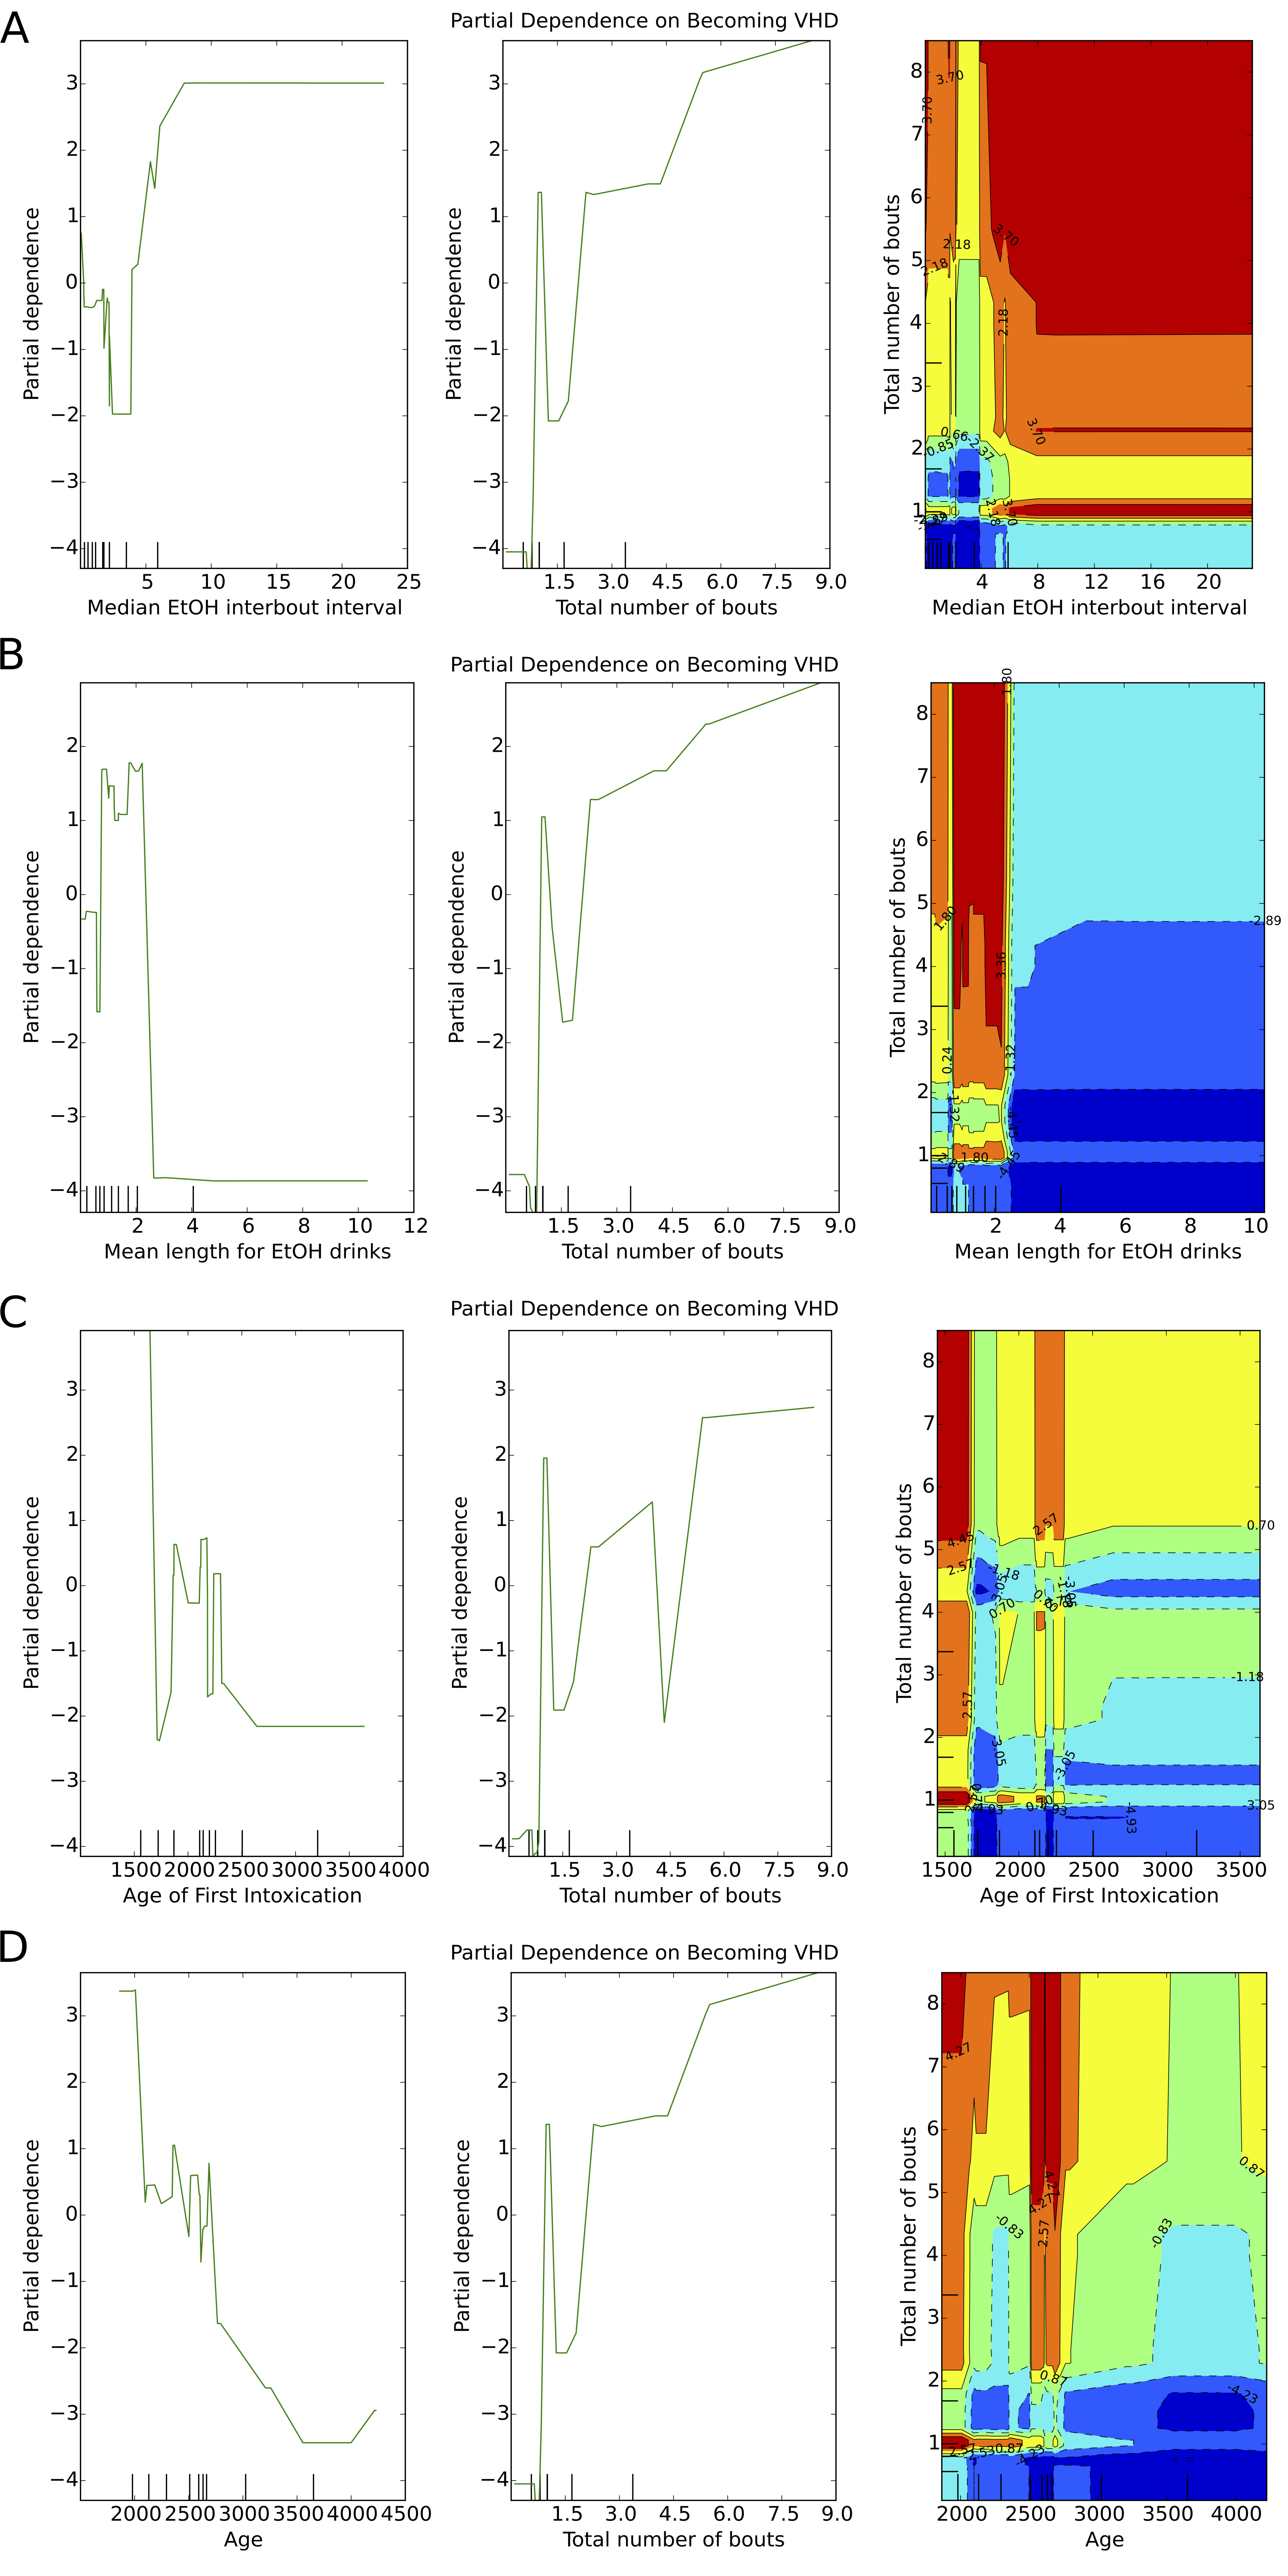
\includegraphics[width=0.7\linewidth]{figures/pdp_vhd.png}
	\caption{Additional PDP gradients of the likelihood of being classified as VHD.}
	\label{fig:VHD_gradients}
\end{figure}

\begin{figure}[ht]
\centering
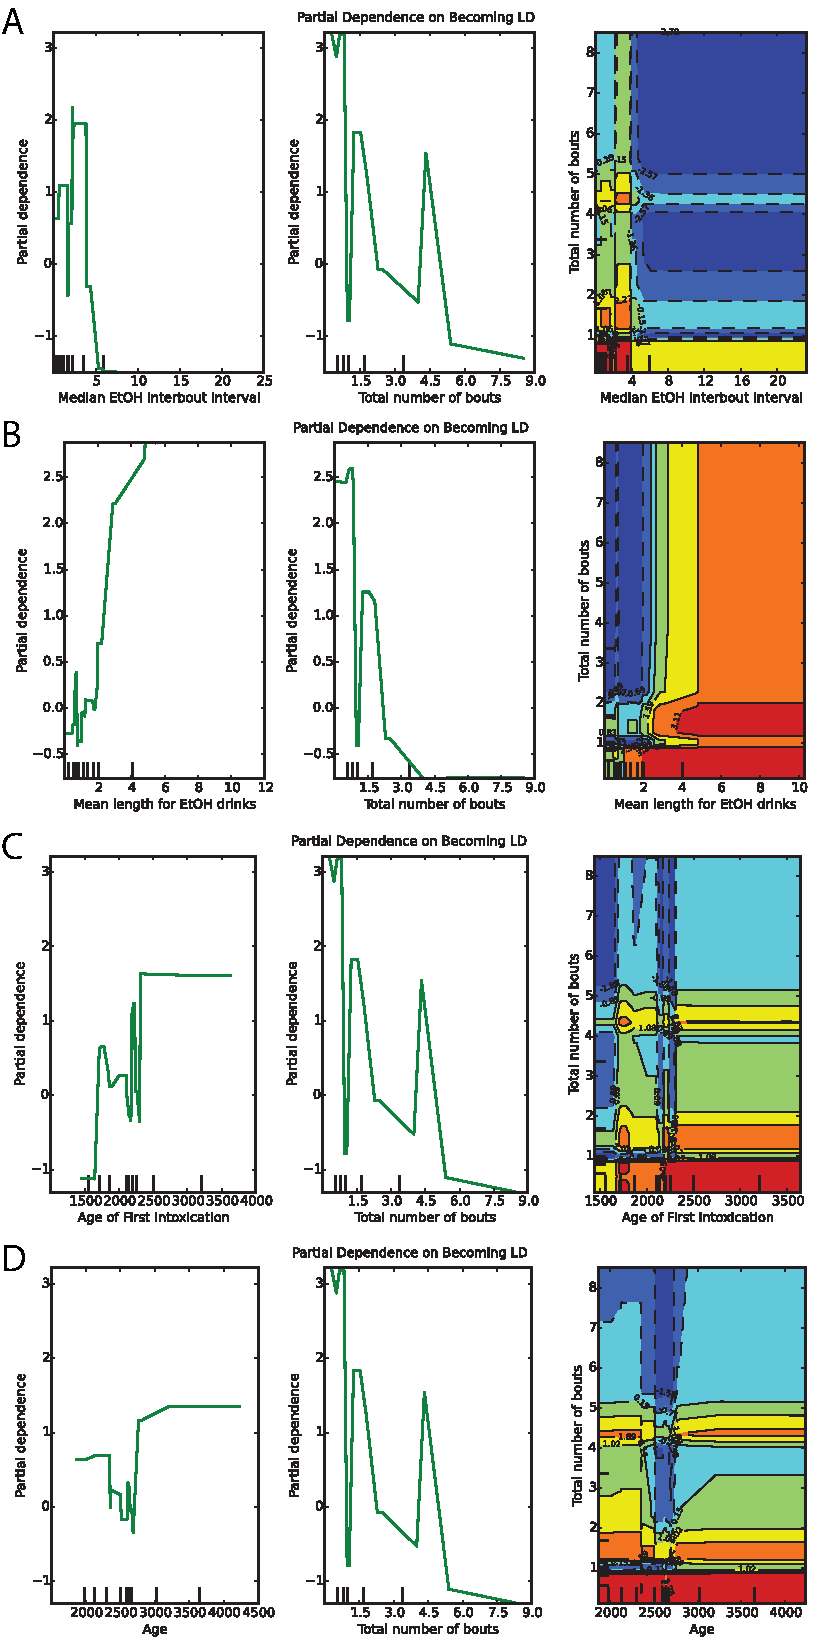
\includegraphics[width=0.7\linewidth]{figures/pdp_ld.pdf}
\caption{Additional PDP gradients of the likelihood of being classified as LD.}
\label{fig:LD_gradients}
\end{figure}

	\end{appendices}
	
	% Bibliography
	\bibliographystyle{chicago} % or whatever style your department uses
	\bibliography{thesis}
	
\end{document}
